% GeoCrop - FYP-1 Mid Report (F26-155)
% Follows the FAST-NUCES F26 FYP-1 Mid Report LaTeX template structure.
\documentclass[12pt,a4paper,twoside,openright]{report}

\usepackage[a4paper,top=1in,bottom=1in,inner=1.15in,outer=1in,headheight=15pt]{geometry}
\usepackage[T1]{fontenc}
\usepackage{times}
\usepackage{setspace}
\usepackage{parskip}
\usepackage{graphicx}
\usepackage{float}
\usepackage{array}
\usepackage{booktabs}
\usepackage{longtable}
\usepackage{tabularx}
\usepackage{multirow}
\usepackage{enumitem}
\usepackage{xcolor}
\usepackage{amsmath}
\usepackage{amssymb}
\usepackage{ragged2e}
\usepackage[font=small,labelfont=bf,skip=6pt]{caption}
\usepackage{tikz}
\usetikzlibrary{arrows.meta,positioning,shapes.geometric,shapes.multipart,fit,calc,backgrounds}
\usepackage{pgfplots}
\pgfplotsset{compat=1.18}
\usepackage{fancyhdr}
\usepackage{emptypage}
\usepackage{url}
\usepackage[colorlinks=true,linkcolor=blue,citecolor=blue,urlcolor=blue]{hyperref}
\hypersetup{pdftitle={GeoCrop: Automated Crop Monitoring and Forecasting Toolkit - FYP-1 Mid Report},
            pdfauthor={Huzaifa Bin Khalid, Saneed Ullah, Taha Bashir Awan}}

\setstretch{1.15}
\setlength{\emergencystretch}{3em}
\setlist{itemsep=2pt,topsep=4pt}
\setcounter{tocdepth}{2}
\setcounter{secnumdepth}{3}
\renewcommand{\arraystretch}{1.18}

% Headers as in the template: chapter on even pages (left), section on odd pages (right).
\pagestyle{fancy}
\fancyhf{}
\renewcommand{\chaptermark}[1]{\markboth{\thechapter.\ #1}{}}
\renewcommand{\sectionmark}[1]{\markright{\thesection\ #1}}
\fancyhead[LE]{\small\nouppercase{\leftmark}}
\fancyhead[RO]{\small\nouppercase{\rightmark}}
\fancyfoot[C]{\thepage}
\renewcommand{\headrulewidth}{0.4pt}
\fancypagestyle{plain}{\fancyhf{}\fancyfoot[C]{\thepage}\renewcommand{\headrulewidth}{0pt}}

\newcolumntype{L}[1]{>{\RaggedRight\arraybackslash}p{#1}}
\newcolumntype{Y}{>{\RaggedRight\arraybackslash}X}
\newcommand{\code}[1]{\expandafter\path\expandafter{\detokenize{#1}}}
\renewcommand{\UrlBreaks}{\do\/\do\_\do\.\do\-\do\:\do\=\do\&\do\,}
\newcommand{\projecttitle}{GeoCrop: Automated Crop Monitoring and Forecasting Toolkit}

% Diagram styles shared by all figures
\tikzset{
  box/.style={draw=black!70, rounded corners=2pt, fill=green!4, align=center, font=\small, inner sep=4pt},
  dbox/.style={draw=black!70, cylinder, shape border rotate=90, aspect=0.18, fill=blue!4, align=center, font=\small, minimum height=1.1cm},
  arr/.style={-{Latex[length=2mm]}, thick, black!70},
  darr/.style={-{Latex[length=2mm]}, thick, dashed, black!60},
  lane/.style={draw=black!40, dashed, rounded corners=3pt},
  lbl/.style={font=\scriptsize, fill=white, inner sep=1pt},
}

\begin{document}

% ------------------------------------------------------------------ title page
\begin{titlepage}
\setstretch{1.0}\setlength{\parskip}{0pt}
\centering
\vspace*{0.6cm}
{\LARGE\bfseries \projecttitle\par}
\vspace{1.0cm}
{\large Project Team\par}
\vspace{0.25cm}
{\Large
\begin{tabular}{ll}
Huzaifa Bin Khalid & 22I-2332\\
Taha Bashir Awan & 23I-0824\\
Saneed Ullah & 23I-2568\\
\end{tabular}\par}
\vspace{0.7cm}
{\large Session 2023-2027\par}
\vspace{0.7cm}
{\large Supervised by\par}
\vspace{0.15cm}
{\Large Mr. Muhammad Aadil Ur Rehman\par}
\vspace{0.45cm}
{\large Co-Supervised by\par}
\vspace{0.15cm}
{\Large Mr. Obaid Ur Rehman\par}
{\normalsize Institute of Space Technology (External)\par}
\vspace{0.7cm}

\includegraphics[width=3.8cm]{figures/fast_logo.png}\par
\vspace{0.6cm}
{\large\bfseries FAST School of Computing\par}
\vspace{0.4cm}
{\large\bfseries National University of Computer and Emerging Sciences\\Islamabad, Pakistan\par}
\vspace{0.4cm}
{\large\bfseries October, 2026\par}
\vspace{0.5cm}
{\small Project ID: F26-155-GeoCrop\par}
\end{titlepage}

% ------------------------------------------------------------------ lists (as placed in the template)
\pagenumbering{arabic}
\setcounter{page}{2}
\pagestyle{plain}
\tableofcontents
\listoffigures
\listoftables

% ------------------------------------------------------------------ front matter
\cleardoublepage
\pagenumbering{roman}
% ------------------------------------------------------------------ Students' Submission
\chapter*{Students' Submission}
\addcontentsline{toc}{chapter}{Students' Submission}
\thispagestyle{plain}
We certify that this report is submitted as the FYP-1 mid-report for the project titled
\textit{\projecttitle}.

\vspace{1.2cm}
\begin{tabular}{p{7cm}l}
Student 1: Huzaifa Bin Khalid (22I-2332) & Signature: \rule{4.5cm}{0.4pt}\\[1.6cm]
Student 2: Taha Bashir Awan (23I-0824) & Signature: \rule{4.5cm}{0.4pt}\\[1.6cm]
Student 3: Saneed Ullah (23I-2568) & Signature: \rule{4.5cm}{0.4pt}\\
\end{tabular}

% ------------------------------------------------------------------ Anti-Plagiarism
\chapter*{Anti-Plagiarism Statement}
\addcontentsline{toc}{chapter}{Anti-Plagiarism Statement}
\thispagestyle{plain}
The students certify that this report is their own work and that all sources used in preparing
the report have been appropriately acknowledged and referenced.

% ------------------------------------------------------------------ Authors' Declaration
\chapter*{Authors' Declaration}
\addcontentsline{toc}{chapter}{Authors' Declaration}
\thispagestyle{plain}
We declare that the work documented in this report represents the work completed by the
project team up to the FYP-1 mid-report stage. Contributions, tools, external components,
and relevant sources are disclosed where applicable, including the use of an AI coding
assistant during platform implementation (Section~\ref{sec:tools-assisted}).

% ------------------------------------------------------------------ Abstract
\chapter*{Abstract}
\addcontentsline{toc}{chapter}{Abstract}
\thispagestyle{plain}
\textbf{Agricultural crop surveys still depend on field visits, manual crop identification and
hand-drawn GIS boundaries, which makes them slow, costly and hard to repeat over large regions.
GeoCrop is a satellite-to-GIS toolkit that learns crop classes from Sentinel-2 imagery and USDA
Cropland Data Layer (CDL) labels, maps cropland and crop types, derives field regions and area,
and will add yield estimation, all presented in a fast Web GIS portal. The research gap is that
existing tools and studies solve crop classification, field mapping or yield prediction in
isolation, and that research prototypes rarely remain usable once many images and model layers
must be displayed. The project follows an iterative plan with two parallel tracks. In Iteration 1
the architecture track replaced the proposal-stage prototype, which sent a 43.3~MB GeoJSON of
101,435 polygons to the browser, with a tile-based platform: Cloud Optimized GeoTIFF results served
by TiTiler, PMTiles vector layers, a React and MapLibre client, a FastAPI service, PostgreSQL with
PostGIS, Celery workers and S3-compatible storage, all run with Docker Compose. One screen of the
same area now costs 337~KB, cold map tiles return in 47~ms (median) and cached tiles in 1~ms, and an
uploaded Sentinel-2 image is processed by both crop models and published to the map in 57~s. A
manifest-based model registry lets new models plug in without changes to the API, database or
interface. The model track evaluated eleven crop-type models on two study areas with a spatial
block test; the proposed LightGBM pipeline with neighbourhood inputs and a 3$\times$3 neighbour vote
reaches 76.1\% accuracy (macro-F1 0.686) in eastern Washington and 92.2\% (macro-F1 0.803) in North
Dakota, while staying about 2~MB and CPU-only. Validation so far covers registry unit tests,
end-to-end API and browser tests, a rendering benchmark and the model evaluation protocol. FYP-2
will integrate the selected crop-type pipeline into the platform, add field-boundary and yield
models, run cross-area tests and prepare deployment.}

% ------------------------------------------------------------------ Acknowledgments
\chapter*{Acknowledgments}
\addcontentsline{toc}{chapter}{Acknowledgments}
\thispagestyle{plain}
The project team acknowledges the guidance and support received from the project supervisor,
Mr. Muhammad Aadil Ur Rehman, the external co-supervisor, Mr. Obaid Ur Rehman (Institute of Space
Technology), the evaluation panel whose proposal feedback shaped this iteration, and the faculty of
the FAST School of Computing. We also acknowledge the open data and open-source communities behind
Sentinel-2, the USDA Cropland Data Layer and the geospatial software used in this project.

% ------------------------------------------------------------------ Executive Summary
\chapter*{Executive Summary}
\addcontentsline{toc}{chapter}{Executive Summary}
\thispagestyle{plain}

\textbf{Project and motivation.} Agriculture departments need to know what is planted, where, over
how much area, and how much may be harvested. Today this comes from physical surveys followed by
manual GIS digitisation, which is time-consuming, resource-intensive and difficult to scale.
GeoCrop automates the chain from satellite imagery to crop maps, field regions, area statistics
and, in FYP-2, yield estimates, and presents them in a Web GIS portal (SDG~2, Zero Hunger).

\textbf{Scope.} The FYP builds a research-grade but usable prototype on open data: Sentinel-2
multispectral imagery as input, the USDA Cropland Data Layer (CDL) as training labels for eight
U.S. areas of interest (AOIs), and USDA NASS statistics for yield. Production-scale national
deployment, cadastral mapping and disease detection are out of scope.

\textbf{Research findings.} Two lines of investigation informed the design. On the platform side,
profiling the proposal prototype showed that its crop-type result for one AOI was a 43.3~MB GeoJSON
with 101,435 polygons (about 750,000 vertices), parsed three times and drawn as SVG, so loading and
zooming were slow and would not scale to more images or models. Keeping model output as rasters and
sending only the map tiles in view removes this cost. On the model side, eleven crop-type models
were compared on AOI1 (eastern Washington, 14 classes) and AOI2 (North Dakota, 9 classes) using
12 monthly Sentinel-2 composites of 2022 and a spatial block split. A time series raised AOI1
accuracy from 26.7\% (one date) to 75.2\%; the model family mattered little (eight models within
2 points); neighbourhood inputs and a 3$\times$3 vote added about 2 points; and 89\% of the remaining
errors sit on field-edge pixels. A small LightGBM model (about 2~MB, CPU-only) was proposed instead of
the much slower Presto foundation model. The proposal was approved with minor modifications; the
panel asked for clearer goals, evaluation criteria that measure performance, light weight, usability
and integration, and a feasibility analysis of the whole workflow. All three are addressed: goals
and criteria were restated with measurable targets, and every workflow stage was measured, showing
that the baseline crop-type model (3.1~GB RAM) is the bottleneck that LightGBM (549~MB) removes.

\textbf{Current implementation.} Iteration 1 delivered a working platform with seven containerised
services: a React and MapLibre Web GIS client, Nginx with a tile cache, a FastAPI service, a
TiTiler tile service, Celery workers, PostgreSQL with PostGIS and MinIO object storage. It supports
browsing and filtering layers, inspecting values at a point, field search, dashboard statistics,
uploading Sentinel-2 imagery, background model runs with live progress, a model catalogue and
system health. A model registry runs the current cropland and crop-type models and lets new models
plug in by folder and manifest.

\textbf{Validation status.} Registry unit tests pass (5/5), including a test that adds a model
without touching other code. End-to-end tests covered every API route, upload to map in 57~s,
crop filtering, field search and inspection in the browser. A benchmark measured 337~KB per screen
against 43.3~MB, cold tiles at 47~ms (median) and cached tiles at 1~ms. Crop-type accuracy is
reported against CDL labels on spatially separated test blocks, with confidence intervals.

\textbf{Risks.} CDL labels are themselves a model output; results cover one year and two areas; the
platform still runs the proposal-stage baseline model until the selected pipeline is integrated;
yield needs reliable historical ground truth; and boundary accuracy is limited at 30~m.

\textbf{Remaining work.} Iteration 2 (end of FYP-1) integrates the LightGBM crop-type pipeline,
adds the CDL confidence filter and a cross-area test, and supports multi-image upload. FYP-2 adds
field-boundary and yield models, an end-to-end evaluation against the success criteria, hardening
and deployment.

% ------------------------------------------------------------------ Abbreviations
\chapter*{List of Abbreviations}
\addcontentsline{toc}{chapter}{List of Abbreviations}
\thispagestyle{plain}
\begin{longtable}{@{}ll@{}}
AOI & Area of Interest\\
API & Application Programming Interface\\
CDL & Cropland Data Layer (USDA)\\
COG & Cloud Optimized GeoTIFF\\
CPU & Central Processing Unit\\
CRS & Coordinate Reference System\\
DEI & Diversity, Equity and Inclusion\\
ERD & Entity Relationship Diagram\\
F1 & Harmonic mean of precision and recall\\
FR & Functional Requirement\\
FYP & Final Year Project\\
GDAL & Geospatial Data Abstraction Library\\
GEE & Google Earth Engine\\
GIS & Geographic Information System\\
JWT & JSON Web Token\\
LightGBM & Light Gradient Boosting Machine\\
MLP & Multi-Layer Perceptron\\
MVT & Mapbox Vector Tile\\
NASS & National Agricultural Statistics Service (USDA)\\
NDVI & Normalized Difference Vegetation Index\\
NFR & Non-Functional Requirement\\
NIR & Near-Infrared\\
OSM & OpenStreetMap\\
PostGIS & Spatial extension for PostgreSQL\\
RAM & Random Access Memory\\
RF & Random Forest\\
S3 & Simple Storage Service (object storage API)\\
SDG & Sustainable Development Goal\\
SUS & System Usability Scale\\
SWIR & Short-Wave Infrared\\
TC & Test Case\\
UC & Use Case\\
USDA & United States Department of Agriculture\\
XYZ & Web map tile addressing scheme (zoom, column, row)\\
\end{longtable}


% ------------------------------------------------------------------ main matter
\cleardoublepage
\pagenumbering{arabic}
\pagestyle{fancy}
\chapter{Introduction and Project Vision}

\section{Project Overview}
GeoCrop is a satellite-based agricultural intelligence toolkit. It takes multispectral satellite
imagery of an agricultural region, identifies which land is cropland, classifies the crop growing
in each 30~m pixel, groups pixels into field regions with area, and (in FYP-2) estimates yield. The
results are published as map layers and statistics in a Web GIS portal, where users can switch
layers on and off, filter by crop, search fields, inspect values at any location and read
crop-area summaries.

The system is built on open data. Sentinel-2~\cite{sentinel2} provides the imagery, the USDA Cropland Data Layer
(CDL)~\cite{cdlsite,lin2022,hao2020} provides labelled crop maps for training and evaluation over eight U.S.
areas of interest (AOIs), and USDA NASS statistics will provide historical yield. GeoCrop is designed
as an academic, department-oriented prototype whose models, evaluation method and outputs are
transparent, and whose software architecture can carry many images and many models without
slowing down.

\section{Problem Statement}
The current crop-survey workflow relies on manual field inspection, crop identification, boundary
digitisation, area calculation and GIS data entry. This process is time-consuming, needs significant
human resources, is difficult to repeat frequently over large regions, and can introduce
inconsistencies in crop classification and field mapping. Satellite imagery observes agricultural
land frequently and with geographic reference, but turning those observations into crop maps,
crop types, field regions, acreage and expected yield still requires substantial processing and
expertise, and the results must be delivered in a form that planners can use interactively over
large areas.

There is therefore a need for an integrated system that learns crop classes from labelled
geospatial data, analyses new satellite imagery, distinguishes cropland from other land, classifies
supported crop types, derives field regions and area, predicts yield from suitable spatio-temporal
features, and presents the results through a responsive Web GIS portal that remains fast as the
number of images and model layers grows.

\section{Problem Context and Motivation}
Agricultural departments, field survey teams, GIS analysts and planners need timely information
about what is planted, where, and over how much area. In the current workflow (physical survey,
crop and non-crop identification, crop-type identification, boundary drawing, area and coordinate
calculation, GIS entry, separate yield assessment) every step is manual. This is slow, needs many
people, is hard to scale across large areas, and can introduce errors.

Open Earth-observation missions now give repeat multispectral coverage, and machine learning has
shown that crop classes can be learned from spectral and temporal patterns~\cite{khan2023,
muqaddas2024,tran2022}. Research in Pakistan confirms that Sentinel-2 can identify crops in
smallholder settings, but still depended on thousands of manually surveyed field boundaries
\cite{khan2023}. In the United States, the CDL offers large labelled coverage that has been used to
train classifiers~\cite{hao2020,wang2020}. GeoCrop uses this labelled coverage to develop and
evaluate the methodology before adaptation to local data.

The motivation is also practical. A crop map is only useful if people can work with it. The
proposal-stage prototype showed that a single AOI's crop-type result, shipped as vector polygons,
already made the map slow to load and zoom. A system meant for many images and several models
(cropland, crop type, boundaries, yield) has to be designed for performance from the start. Better
agricultural monitoring supports informed crop planning and food-security decisions (SDG~2,
Zero Hunger).

\section{Project Vision}
GeoCrop aims to give agricultural organisations a single toolkit that turns new satellite imagery
into trustworthy, map-ready crop intelligence in minutes: where the cropland is, what is growing,
how large each crop area is, and what yield to expect. Results should be honest about their
accuracy, reproducible, and fast to explore on a map, and new models should plug into the same
platform as research progresses.

\section{Project Objectives}\label{sec:goals}
After the proposal defence the panel asked the team to clarify its goals (P1,
Section~\ref{sec:feedback}). The goals are now stated as follows. GeoCrop's primary goal is a
\emph{light, fast and integrated} platform: one that turns an uploaded Sentinel-2 image into crop
layers on a map without heavy hardware, and that stays usable as images and models grow. Its
research goal is crop-type models that are accurate under a fair test and cheap enough to serve.
Three terms from the proposal are defined precisely:
\begin{itemize}
  \item \textbf{Crop mapping}: per-pixel cropland and crop-type maps at 30~m for supported AOIs,
        scored against the CDL on spatially separated test blocks.
  \item \textbf{GIS integration}: every result is a georeferenced layer in one catalogue, viewable,
        filterable and comparable on the same map as the imagery and other layers.
  \item \textbf{Real-time estimation}: \emph{near} real time on demand. An AOI-sized image is analysed
        and published in about a minute (57~s measured), and a map screen loads in well under a
        second. Continuous streaming of new imagery is not a goal.
\end{itemize}
Each objective below has a measurable target that is checked in Chapter~7.
\begin{enumerate}[label=\textbf{O\arabic*.}, leftmargin=1.1cm]
  \item Build a spatially aligned Sentinel-2 and CDL training dataset for at least two AOIs, with
        a reproducible preparation pipeline.
  \item Develop and evaluate cropland and crop-type models using a spatially separated test set,
        reporting accuracy, macro-F1 and per-class scores with confidence intervals, and compare
        them with published results.
  \item Derive field regions and area from model output and publish them as GIS layers with
        geographic coordinates; add a dedicated field-boundary model in FYP-2.
  \item Develop a yield-estimation module evaluated with $R^2$, RMSE and MAE against USDA NASS
        records at the spatial scale for which ground truth exists.
  \item Deliver a Web GIS portal that shows one screen of results using under 1~MB of data, returns
        cold map tiles in under 300~ms and cached tiles in under 50~ms, and keeps several layers
        visible at once.
  \item Provide a processing pipeline in which an uploaded image is validated, analysed by the
        selected models and published to the map automatically, and in which a new model can be
        added without changing the API, database schema or user interface.
\end{enumerate}

\section{Project Scope}
\textbf{Included.}
\begin{itemize}
  \item Satellite data preparation: Sentinel-2 composites, band selection, reprojection to the
        CDL grid, vegetation indices and monthly time series.
  \item CDL-based label preparation for the supplied AOIs, including rare-class grouping.
  \item Cropland/non-cropland and multi-class crop-type mapping with model comparison.
  \item Field-region derivation, area statistics and vector map layers; a field-boundary model in
        FYP-2.
  \item Yield estimation using satellite features and USDA NASS history (FYP-2).
  \item A Web GIS platform: upload and processing jobs, layer catalogue, tile-based map, dashboard,
        model catalogue, system status, and user accounts.
\end{itemize}
\textbf{Excluded.} Building or operating satellites; legal or cadastral ownership mapping; crop
disease diagnosis; real-time farm machinery integration; production-scale national deployment
with service-level guarantees; and claims of ground-truth accuracy beyond agreement with the
reference labels.

\section{Project Modules}
\begin{table}[htbp]
\centering\small
\caption{GeoCrop modules and responsibilities}
\label{tab:modules}
\begin{tabularx}{\textwidth}{L{4.2cm} Y L{2.2cm}}
\toprule
\textbf{Module} & \textbf{Responsibility} & \textbf{Status}\\
\midrule
M1 Data acquisition and preprocessing & Export Sentinel-2 composites, align them to the CDL grid (EPSG:5070, 30~m), build monthly time series and indices, convert results to Cloud Optimized GeoTIFF. & Working for AOI1, AOI2\\
M2 Crop mapping & Cropland/non-cropland and crop-type models; evaluation and model selection. & Baseline in platform; research pipeline selected\\
M3 Field regions, boundaries and area & Polygonise model output, compute area, build vector tiles; field-boundary model later. & Field regions working; model in FYP-2\\
M4 Yield estimation & Regression on satellite features and NASS yield history. & FYP-2 (registered placeholder)\\
M5 Processing pipeline & Upload, validation, preprocessing, background model runs, progress tracking. & Working\\
M6 Model registry & Plug-in contract, manifests, dependency resolution, model catalogue. & Working\\
M7 Catalogue, storage and statistics & PostGIS catalogue of areas, runs, layers, statistics and fields; S3 object storage. & Working\\
M8 Web GIS portal & Home, Live Map, Dashboard, Analyze Imagery, Models, System Status, accounts. & Working\\
\bottomrule
\end{tabularx}
\end{table}

\section{Stakeholders and User Classes}
\begin{table}[htbp]
\centering\small
\caption{Stakeholders and user classes}
\label{tab:stakeholders}
\begin{tabularx}{\textwidth}{L{4.2cm} Y}
\toprule
\textbf{Stakeholder / user class} & \textbf{Characteristics and needs}\\
\midrule
Agriculture Department & Needs regional crop area and expected production for planning; values accuracy and transparency.\\
Field survey teams & Today collect crop and boundary data manually; benefit from fewer field visits and targeted checks.\\
GIS analysts & Technical users; need georeferenced layers, coordinates, area and exportable data.\\
Agricultural planners and decision makers & Non-technical; need clear maps, legends and summary statistics.\\
Farmers & Indirect beneficiaries of better planning and advisory services.\\
Industry / startup partner & External collaborator interested in a scalable, light system.\\
Platform developers and ML engineers & Add and update models, monitor the system, run evaluations.\\
\bottomrule
\end{tabularx}
\end{table}

\section{Success Criteria}
\begin{itemize}
  \item \textbf{Crop mapping:} crop-type accuracy and macro-F1 reported on spatially separated test
        blocks with 95\% intervals; results comparable in order of magnitude to published CDL-based
        studies for similar regions (for example 94\% South Dakota and 83\% California
        in~\cite{tran2022}).
  \item \textbf{Boundaries and area:} spatial overlap (IoU) and area error against reference data,
        and acreage within a stated tolerance of USDA statistics (FYP-2).
  \item \textbf{Yield:} $R^2$, RMSE and MAE on held-out years or counties (FYP-2).
  \item \textbf{Performance:} first visible result under 1~s, under 1~MB per screen, cold tiles
        under 300~ms, cached tiles under 50~ms, eight or more layers visible.
  \item \textbf{Pipeline:} an uploaded image reaches the map without manual steps, with readable
        errors for invalid input; a new model is added by folder and manifest only.
  \item \textbf{Lightweight:} the full workflow runs on one laptop-class host; the selected crop-type
        model is CPU-only and small; peak memory per stage is measured.
  \item \textbf{Usability:} non-technical users can find, filter and read results using legends and
        plain-language labels; measured with task completion and a questionnaire score in a user
        study.
  \item \textbf{Integration:} several layers from different models and images can be used together on
        one map without loading whole datasets.
\end{itemize}

\section{Constraints and Assumptions}
\begin{itemize}
  \item CDL labels are a classified product, not field survey data; scores measure agreement with
        the CDL~\cite{lin2022}.
  \item Sentinel-2 at 10--20~m, resampled to the 30~m CDL grid, limits boundary precision for small
        fields.
  \item Data for 2022 is used so that imagery and labels refer to the same season.
  \item Yield ground truth (USDA NASS) is available at county level, which bounds the spatial scale
        of yield evaluation.
  \item Compute is limited to student laptops and free cloud notebooks, and the panel named a
        lightweight system as a main concern, so CPU-only inference is preferred and resource use
        is measured for every stage (Section~\ref{sec:feasibility}).
  \item Uploaded imagery is assumed to be a georeferenced Sentinel-2 surface-reflectance stack with
        the documented bands; other formats are rejected with a clear message.
  \item The platform runs on Docker Compose on a single host for development and demonstration.
\end{itemize}

\section{Ethical, Legal and DEI Considerations}
\begin{itemize}
  \item \textbf{Honest reporting:} predictions are never presented as ground truth. The portal
        shows model accuracy, its evaluation protocol and limitations; placeholder models are
        labelled ``coming soon'' and never produce data.
  \item \textbf{Fairness across classes and regions:} per-class scores and per-area results are
        reported so that unequal performance (for example on small or rare crops) is visible.
  \item \textbf{Licensing:} Sentinel-2 data (Copernicus open licence), CDL and NASS data (U.S.
        public domain), OpenStreetMap basemap (ODbL attribution shown) and open-source libraries
        are used within their terms and acknowledged.
  \item \textbf{Privacy:} uploaded imagery and results belong to the uploading account; passwords
        are hashed; startup-provided data will be protected and not published.
  \item \textbf{Accessibility and inclusion:} the interface uses clear legends, plain-language
        labels, keyboard-accessible controls and readable colour palettes so that technical and
        non-technical staff can use it.
  \item \textbf{Disclosure:} external datasets, models, libraries and AI-assisted work are
        disclosed (Sections~\ref{sec:tools-assisted} and~\ref{sec:external}).
\end{itemize}

\chapter{Research and Existing Solutions}

\section{Research Method / Approach}
Knowledge was built along four lines.
\begin{enumerate}
  \item \textbf{Literature review.} Studies on CDL-based crop classification, crop mapping in
        Pakistan, field-boundary extraction, yield prediction and time-series deep learning were
        reviewed (Table~\ref{tab:literature}). Eight further papers were read for the crop-type
        comparison (Section~\ref{sec:papers}).
  \item \textbf{Data analysis.} The supplied CDL rasters and AOI shapefiles were analysed for class
        distribution, field layout and edge pixels; Sentinel-2 composites were exported with Google
        Earth Engine and aligned to the CDL grid.
  \item \textbf{Controlled experiments.} Crop-type models were compared under one protocol: 12
        monthly composites of 2022, a spatial block split with a buffer, normalisation on training
        data only, and all choices made on validation data (Chapter~\ref{ch:iter1}).
  \item \textbf{Engineering investigation.} The proposal-stage prototype was profiled to find its
        performance limits, candidate geospatial technologies were compared, and the chosen design
        was benchmarked on the real AOI1 data.
\end{enumerate}

\section{Existing Solutions / Products}
\textbf{USDA CropScape / CDL} provides annual georeferenced crop maps and acreage statistics for the
United States. It is an already-classified product and does not analyse new imagery supplied by a
user, estimate yield, or provide a configurable workflow.

\textbf{QGIS and ArcGIS-type GIS tools} visualise geospatial data, edit polygons, calculate area and
manage coordinates. Crop identification and yield prediction still require separate data, models and
expert workflows.

\textbf{DSSAT crop models} simulate crop growth and estimate yield from agronomic and environmental
inputs. They do not classify crops from satellite imagery or extract field regions.

\textbf{OneSoil and similar precision-agriculture platforms} combine satellite imagery, vegetation
indices and field monitoring in a map interface~\cite{onesoil2026}. They are commercial and
closed, so models, training data and accuracy are not transparent or adaptable to a department's
data.

\textbf{Prior FYPs} typically address one task: crop classification (model accuracy only), GIS or
field mapping (classification supplied manually), or yield prediction (no automatic crop mapping or
boundaries).

\textbf{Research literature.} Table~\ref{tab:literature} summarises the most relevant studies.

\begingroup\small
\begin{longtable}{L{0.45cm} L{2.8cm} L{1.9cm} L{4.1cm} L{4.0cm}}
\caption{Summary of literature and gaps for GeoCrop}\label{tab:literature}\\
\toprule
\textbf{No.} & \textbf{Paper / year} & \textbf{Focus} & \textbf{Key contribution} & \textbf{Gap for GeoCrop}\\
\midrule\endfirsthead
\toprule
\textbf{No.} & \textbf{Paper / year} & \textbf{Focus} & \textbf{Key contribution} & \textbf{Gap for GeoCrop}\\
\midrule\endhead
\midrule\multicolumn{5}{r}{\textit{Continued on next page}}\\\endfoot
\bottomrule\endlastfoot
1 & Lin et al.\ 2022~\cite{lin2022} & CDL refinement & Spatial-temporal decision tree flags and corrects questionable CDL pixels; pixel and county validation. & Shows CDL label noise at edges; no new-image classification or yield.\\
2 & Hao et al.\ 2020~\cite{hao2020} & CDL transfer learning & High-confidence CDL pixels with Landsat/Sentinel NDVI time series train Random Forests (OA 86--98\%). & Classification only; no GIS boundary or yield workflow.\\
3 & Tran et al.\ 2022~\cite{tran2022} & 10~m crop type from CDL & Monthly Sentinel-2 composites and good-quality CDL samples; OA 94\% (South Dakota), 83\% (California). & Random sample split and quality filtering; no platform.\\
4 & Wang et al.\ 2020~\cite{wang2020} & Historical mapping & CDL labels with Landsat reconstruct 20 years of corn and soybean in the Midwest. & Two crops only; no integrated portal.\\
5 & Khan et al.\ 2023~\cite{khan2023} & Punjab crop ID & Stacked LSTM on Sentinel-2 time series for rice, wheat, sugarcane. & Relies on GPS ground surveys; no boundaries or yield.\\
6 & Latif et al.\ 2023~\cite{latif2023} & Pakistan cropland & Multi-date Sentinel-2 and ML on Google Earth Engine for cropland extent. & Cropland only; no crop types or yield.\\
7 & Muqaddas et al.\ 2024~\cite{muqaddas2024} & Punjab sugarcane & Deep learning on Sentinel-2 indices; cross-district tests. & Single crop; no integrated workflow.\\
8 & Edri et al.\ 2026~\cite{edri2026} & Field boundaries & SAM, U-Net, DeepLabV3, SegFormer on time series refine field polygons. & Assumes a parcel registry; no crop type or yield.\\
9 & Desloires et al.\ 2023~\cite{desloires2023} & Corn yield & Sentinel-2 and environmental features; out-of-year evaluation. & Assumes known fields and yield labels.\\
10 & Xiao et al.\ 2024~\cite{xiao2024} & Wheat yield & Attention 1D CNN on Sentinel-2 time series. & Single crop; no mapping.\\
11 & You et al.\ 2017~\cite{you2017} & County yield & Deep Gaussian process on remote-sensing histograms. & County level; no field mapping.\\
12 & Zhang et al.\ 2025~\cite{zhang2025} & Within-season U.S. crop type & Transformer on HLS time series, CDL labels, 37 crop types. & Large model (about 17~M parameters); research code only.\\
13 & Li et al.\ 2024~\cite{li2024} & In-season CDL & Trusted pixels from CDL history, Random Forest; corn/soy F1 0.85--0.97. & No user-facing workflow.\\
14 & Tseng et al.\ 2023~\cite{tseng2023} & Presto & Light pre-trained transformer for pixel time series. & Benefit shown mostly with few labels.\\
15 & Szwarcman et al.\ 2024~\cite{szwarcman2024} & Prithvi-EO-2.0 & 300--600~M parameter foundation model; crop segmentation mIoU up to 50.7. & Too heavy for a light CPU system.\\
\end{longtable}
\endgroup

\section{Comparison of Existing Solutions}
\begin{table}[htbp]
\centering\small
\caption{Comparison of existing solutions with GeoCrop on project-relevant criteria}
\label{tab:compare}
\begin{tabular}{L{3.6cm} *{6}{>{\centering\arraybackslash}p{1.45cm}}}
\toprule
\textbf{Solution} & \textbf{Classifies new imagery} & \textbf{Field regions / area} & \textbf{Yield} & \textbf{Web map} & \textbf{Open / transparent} & \textbf{Scales to many layers}\\
\midrule
USDA CropScape / CDL & -- & partial & -- & \checkmark & \checkmark & \checkmark\\
QGIS / ArcGIS & -- & \checkmark & -- & partial & partial & partial\\
DSSAT & -- & -- & \checkmark & -- & \checkmark & --\\
OneSoil-type platforms & \checkmark & \checkmark & partial & \checkmark & -- & \checkmark\\
Prior FYPs & partial & partial & partial & partial & \checkmark & --\\
GeoCrop proposal prototype & \checkmark & partial & -- & \checkmark & \checkmark & --\\
\textbf{GeoCrop (this work)} & \checkmark & \checkmark & FYP-2 & \checkmark & \checkmark & \checkmark\\
\bottomrule
\end{tabular}
\end{table}

\section{Limitations and Gaps}
\begin{itemize}
  \item \textbf{Fragmented workflows.} Crop classification, field mapping and yield prediction are
        usually separate tools or studies; users must combine them by hand.
  \item \textbf{Dependence on manual surveys.} Local studies rely on GPS field surveys
        \cite{khan2023}; CDL supervision reduces the labels needed for early development.
  \item \textbf{Optimistic evaluation.} Many studies use random pixel or sample splits. Our own test
        showed that a random split leaks neighbouring pixels (macro-F1 0.396 random against 0.147
        with blocks on the same model), so published numbers are not always comparable.
  \item \textbf{Prototypes that do not scale.} Research outputs are often shipped as large vector
        files. The proposal prototype needed 43.3~MB and 101,435 SVG polygons for one AOI's crop-type
        layer, which made the map slow and would not scale to several images and models.
  \item \textbf{Heavy models.} Foundation models are accurate but need hundreds of megabytes or GPUs,
        which conflicts with a light, affordable system.
  \item \textbf{Label uncertainty.} CDL contains mixed-pixel and boundary errors~\cite{lin2022}, which
        must be accounted for in training and reporting.
\end{itemize}

\section{Proposed Solution}
GeoCrop connects the tasks into one satellite-to-GIS workflow and builds it on an architecture
designed for performance and change:
\begin{itemize}
  \item \textbf{Raster-first results served as tiles.} Model outputs are stored as Cloud Optimized
        GeoTIFFs and served as small map tiles by TiTiler; vector field regions are packed as
        PMTiles. The browser downloads only what is on screen.
  \item \textbf{A plug-in model registry.} Cropland, crop-type, boundary and yield models share one
        contract; dependencies run in order; new models are added by folder and manifest.
  \item \textbf{An asynchronous processing pipeline.} Uploads go straight to object storage; Celery
        workers validate, preprocess, run models and publish each layer with statistics.
  \item \textbf{A transparent, light crop-type model.} A LightGBM pipeline on monthly Sentinel-2
        composites with neighbourhood inputs and a neighbour vote, evaluated with a spatial block
        split and reported with intervals and per-class scores.
  \item \textbf{A usable portal.} Layer panel, crop filter, field search, point inspection,
        dashboard, model catalogue and system health in one interface.
\end{itemize}

\section{Complex Computing Problem}
Under the Seoul Accord definition~\cite{seoulaccord2026}, GeoCrop is a complex computing problem: it
has no obvious solution, combines several knowledge areas and has interdependent parts.
\begin{table}[htbp]
\centering\small
\caption{Mapping of GeoCrop components to complex computing problem attributes}
\label{tab:ccp}
\begin{tabularx}{\textwidth}{L{3.8cm} Y}
\toprule
\textbf{Component} & \textbf{Attributes and evidence}\\
\midrule
Crop mapping and classification & \textit{Conflicting requirements} (accuracy against model size, speed and cost); \textit{depth of analysis} (no single best model: eleven compared, label noise, edge pixels); \textit{depth of knowledge} (ML, multispectral remote sensing, phenology); \textit{interdependence} (preprocessing and label alignment drive accuracy).\\
\addlinespace
Field regions, boundaries and area & \textit{Depth of knowledge} (CRS, raster/vector processing, area in projected units); \textit{interdependence} (crop-map errors propagate to polygons and acreage); \textit{consequences} (wrong acreage misleads planning).\\
\addlinespace
Yield estimation & \textit{Depth of analysis} (temporal features, scale of ground truth); \textit{consequences} (production forecasts); \textit{conflicting requirements} (granularity against available labels).\\
\addlinespace
Platform and rendering & \textit{Conflicting requirements} (detail against speed and data volume); \textit{depth of knowledge} (COG, tiling, vector tiles, spatial databases, distributed jobs); \textit{stakeholder needs} (technical and non-technical users); \textit{interdependence} (every model output must become a correct, fast layer).\\
\bottomrule
\end{tabularx}
\end{table}

\section{Technical Challenges}
\begin{itemize}
  \item \textbf{Rendering performance.} Pixel-level predictions vectorised into polygons produce very
        large files (101,435 polygons for one AOI). Displaying many images and layers requires
        tiling, caching and immutable versioned URLs.
  \item \textbf{Spatial alignment.} Sentinel-2 (10--20~m, UTM) must be reprojected exactly onto the
        CDL grid (EPSG:5070, 30~m); web maps use EPSG:3857.
  \item \textbf{Label noise and edge pixels.} In AOI1, 47\% of test pixels touch another class and
        hold 89\% of the errors; CDL itself is noisy there.
  \item \textbf{Evaluation leakage.} Random pixel splits overstate accuracy; spatial blocks with a
        buffer are needed.
  \item \textbf{Cloud gaps.} Missing monthly observations must be filled consistently.
  \item \textbf{Model size and speed.} The default Random Forest is 328~MB; the baseline crop-type
        model in the platform is 1.5~GB and must be loaded per run; Presto is 660 times slower than
        an MLP.
  \item \textbf{Integration.} Model outputs, statistics, styles and files must stay consistent across
        the database, object storage, tile service and client.
  \item \textbf{Operations.} Container start-up races, service discovery after rebuilds and browser
        caching had to be handled for a reliable demonstration.
\end{itemize}

\section{Research Findings and Design Decisions}
\begin{table}[htbp]
\centering\small
\caption{How research findings shaped design decisions}
\label{tab:findings}
\begin{tabularx}{\textwidth}{L{6.4cm} Y}
\toprule
\textbf{Finding} & \textbf{Decision}\\
\midrule
One AOI's crop-type GeoJSON was 43.3~MB with 101,435 polygons; parsing alone took about 1~s. & Keep results as rasters (COG); serve XYZ tiles with TiTiler; vectors only as PMTiles.\\
Most of the prototype polygons (85\%) were single-pixel squares. & Raster is the source of truth; polygons are derived, filtered by minimum size and simplified per zoom.\\
A time series lifted AOI1 accuracy from 26.7\% to 75.2\%. & Use 12 monthly composites of the label year as model input.\\
Eight model families finished within 2 points; logistic regression 4.8 points behind. & Choose the model on cost: LightGBM (about 2~MB, CPU); keep Random Forest as baseline.\\
Presto matched simple models but was about 660 times slower per pixel. & Reverse the earlier Presto recommendation for the U.S./CDL case.\\
Random pixel splits leak neighbours (macro-F1 0.396 against 0.147). & Spatial 100$\times$100 block split, 3-pixel buffer, choices on validation only.\\
89\% of errors are on field-edge pixels. & Neighbourhood inputs and a 3$\times$3 vote now; field-level classification later.\\
Models and outputs will keep changing (cropland, crop type, boundary, yield). & Manifest-based model registry with a dependency graph and generic layer catalogue.\\
Heavy work (image conversion, inference) takes tens of seconds. & Asynchronous Celery jobs with progress; direct-to-storage uploads.\\
\bottomrule
\end{tabularx}
\end{table}

\chapter{Proposal Feedback and Iteration Plan}

\section{Proposal Feedback Summary}\label{sec:feedback}
The proposal defence result was sent by the FYP Committee on 14 September 2026. The decision for
F26-155-GeoCrop was \textbf{Approved with Minor Modifications}. The panel's comments are summarised
below; each is numbered P1--P7 and tracked in the action register.
\begin{enumerate}[label=\textbf{P\arabic*.}, leftmargin=1.1cm]
  \item \textbf{Clarify the intended goals.} The proposal claimed crop mapping, GIS integration and
        real-time estimation without stating clearly what each meant.
  \item \textbf{Improve the evaluation metrics.} The proposed criteria did not measure the actual
        challenges of the project.
  \item \textbf{Measure the real challenges: computational performance, a lightweight system and
        usability.} The panel stated that the evaluation criteria were wrong, and that usability,
        performance and integration are the main concerns.
  \item \textbf{Analyse feasibility.} The complexity and resource requirements of the complete
        workflow had not been analysed beforehand.
  \item \textbf{Do not run everything in a single flow.} The computational and space requirements are
        high enough that running the entire process in a single flow may not be practical.
  \item \textbf{Integration of huge datasets.} Large datasets are not easy to load and use together.
  \item \textbf{Work on presentation skills.}
\end{enumerate}
The panel also asked the team to incorporate all changes it suggested. These comments set the agenda
for Iteration 1. The architecture track answered P3--P6 by redesigning the platform around
performance, light weight and integration, and measuring each one. The model track answered P2--P4
by changing the evaluation protocol and selecting the model on cost as well as accuracy.

The team's own review after the defence found further issues: the prototype could not run models on
uploaded images, the first evaluation used an optimistic random pixel split, models would keep
changing during the project, and the iteration plan in the proposal slides no longer matched the
order in which the work had to be done. These items are recorded separately in the register, with
their source.

\section{Proposal Action Register}
\begin{table}[htbp]
\centering\small
\caption{Proposal action register (summary; full register with evidence in Appendix~\ref{app:register})}
\label{tab:register}
\begin{tabularx}{\textwidth}{L{0.8cm} L{3.6cm} Y L{1.3cm} L{1.7cm}}
\toprule
\textbf{No.} & \textbf{Feedback / required change} & \textbf{Action taken} & \textbf{Status} & \textbf{Evidence}\\
\midrule
P1 & Clarify the intended goals. & Objectives restated with measurable targets; ``real-time'' defined as an uploaded image on the map in about a minute; scope split by FYP phase. & Done & Sec.~\ref{sec:goals}\\
P2, P3 & Evaluation metrics must measure performance, light weight, usability and integration. & Evaluation criteria rewritten around these concerns, each with a metric and target. Performance, cost and integration measured; usability checked against requirements, user study planned. & Partly done & Table~\ref{tab:evalcriteria}\\
P4 & Analyse feasibility and resource requirements of the whole workflow. & Time, memory and storage measured for every stage; the baseline crop-type model (3.1~GB RAM) found to dominate, so it is replaced by LightGBM (549~MB). & Done & Table~\ref{tab:resources}\\
P5 & A single-flow process is not practical. & Workflow split into independent queued stages; results kept as compressed rasters; maps served tile by tile on demand. & Done & Sec.~\ref{sec:feasibility}\\
P6 & Huge datasets are hard to load and use together. & Only visible tiles are sent: 337~KB per screen instead of 43.3~MB; layers share one catalogue. & Done & Table~\ref{tab:benchmark}\\
P7 & Presentation skills. & Fixed demonstration script on the running system; each member presents their own track; rehearsals before evaluations. & In progress & Sec.~\ref{sec:demo}\\
T1 & Team review: uploaded images were never analysed. & Upload, validation, preprocessing and model runs as background jobs; 57~s upload-to-map. & Done & TC-11, Fig.~\ref{fig:seq}\\
T2 & Team review: random pixel split overstates accuracy. & Spatial block split with buffer; choices on validation; intervals over test blocks. & Done & Sec.~\ref{sec:protocol}\\
T3 & Team review: models will keep changing. & Manifest-based model registry; add-a-model test. & Done & TC-03\\
T4 & Team review: iteration plan in the slides outdated. & Two-track iteration plan (Sections~\ref{sec:it1plan}, \ref{sec:it2plan}, Chapter~\ref{ch:remaining}). & Done & This chapter\\
\bottomrule
\end{tabularx}
\end{table}

\section{Iteration Strategy}
Development is iterative and time-boxed. Each iteration ends with a working, demonstrable increment,
a short evaluation, and an updated plan. Because GeoCrop has two kinds of risk, work proceeds on two
parallel tracks that meet at the end of each iteration:
\begin{itemize}
  \item \textbf{Architecture track} (platform): data flow, storage, processing, map delivery and
        interface. Risk: performance and integration.
  \item \textbf{Model track} (research): data preparation, model comparison and evaluation. Risk:
        accuracy, generalisation and cost.
\end{itemize}
The two tracks share one contract: a model is a plug-in that reads an aligned image and writes a
georeferenced raster, so research results can move into the platform without redesign.
Decisions are made on measured evidence (benchmarks for the platform, validation scores for models)
and recorded in this report and the repository.

\begin{table}[htbp]
\centering\small
\caption{Updated iteration plan (replaces the phase plan presented in the proposal slides)}
\label{tab:iterations}
\begin{tabularx}{\textwidth}{L{2.4cm} L{2.6cm} Y}
\toprule
\textbf{Iteration} & \textbf{Period} & \textbf{Focus}\\
\midrule
Iteration 1 & Sep -- mid-Oct 2026 (FYP-1, to mid-term) & Base architecture with implementation and performance benchmark; crop-type model evaluation and comparison.\\
Iteration 2 & mid-Oct -- Dec 2026 (FYP-1, to final) & Integrate the selected crop-type pipeline into the platform; CDL confidence rule; cross-area test; multi-image upload.\\
Iteration 3 & Feb -- Mar 2027 (FYP-2) & Field-boundary model and area validation; yield data and first yield model; more AOIs.\\
Iteration 4 & Apr -- May 2027 (FYP-2) & End-to-end evaluation, hardening, deployment and final documentation.\\
\bottomrule
\end{tabularx}
\end{table}

\section{Iteration 1 Plan}\label{sec:it1plan}
\textbf{Objectives.} (1) Replace the prototype with a base architecture that stays fast as images and
models grow, implemented and benchmarked on real data. (2) Find a crop-type model that is accurate
under a fair test and light enough for the platform.

\textbf{Selected features.} Tile-based Live Map with layer panel, opacity, legends, crop filter,
field search and point inspection; dashboard statistics from the database; upload and background
processing with progress; model registry with the current cropland and crop-type models;
system-status page. On the model side: monthly composites for AOI1 and AOI2, eleven-model
comparison, improvement ladder, error analysis and comparison with published papers.

\textbf{Deliverables.} Platform repository with Docker Compose stack and documentation; benchmark
results; crop-type results report; this mid-report.

\textbf{Evidence.} Benchmark tables, test results, screenshots (Section~\ref{sec:demo}) and
repository history (Appendix~\ref{app:repo}).

\section{Iteration 2 Plan}\label{sec:it2plan}
\textbf{Objectives.} Bring the selected crop-type pipeline into the platform and strengthen the
evaluation.

\textbf{Selected features.}
\begin{itemize}
  \item Package the LightGBM pipeline (monthly composites, neighbourhood inputs, 3$\times$3 vote) as a
        registry model and replace the baseline crop-type model in the platform.
  \item Monthly-composite ingestion in the processing pipeline.
  \item Fix one CDL confidence rule and report it next to the all-pixel score; compute the AOI2
        interval and interior table.
  \item Cross-area test (train on one AOI, test on the other).
  \item Multi-image upload and an ``all areas'' map view.
  \item Measure end-to-end serving cost of the improved pipeline on CPU and repeat the workflow
        resource measurement (Table~\ref{tab:resources}).
  \item Usability study: task-based sessions with a questionnaire score and task times (P3).
  \item Multi-layer test: eight or more layers visible at once (NFR-P3).
\end{itemize}
\textbf{Deliverables.} Updated platform release, evaluation addendum and FYP-1 final report.
\textbf{Evidence.} Test results, benchmark re-run and model cards with stored metrics.

\section{Work Breakdown and Responsibilities}
\begin{table}[htbp]
\centering\small
\caption{Work breakdown and ownership}
\label{tab:wbs}
\begin{tabularx}{\textwidth}{L{3.4cm} Y L{3.5cm}}
\toprule
\textbf{Work package} & \textbf{Tasks} & \textbf{Owner}\\
\midrule
WP1 Architecture and platform & Architecture design; performance analysis of the prototype; tile serving; storage and database design; processing pipeline; model registry; web portal; deployment configuration; benchmark. & Huzaifa Bin Khalid\\
WP2 Crop-type model evaluation & Monthly composite preparation; spatial block protocol; model comparison and cost measurement; improvement ladder; error analysis. & Saneed Ullah, Taha Bashir Awan\\
WP3 Comparison with literature & Reading and checking reference papers; like-for-like comparison and limits. & Saneed Ullah, Taha Bashir Awan\\
WP4 Integration (Iteration 2) & Packaging the selected model as a registry plug-in; end-to-end measurement. & Shared\\
WP5 Documentation and evaluation & Reports, demonstrations, final evaluation. & Shared\\
\bottomrule
\end{tabularx}
\end{table}

\section{Progress Against Plan}
\begin{table}[htbp]
\centering\small
\caption{Planned phases (proposal slides) against actual progress}
\label{tab:progress}
\begin{tabularx}{\textwidth}{L{3.3cm} L{4.5cm} Y}
\toprule
\textbf{Planned (slides)} & \textbf{Planned content} & \textbf{Actual at mid-term}\\
\midrule
Phase 1 (FYP-1) Research and data understanding & Literature review; CDL/AOI analysis; satellite data acquisition & Done. Literature extended with eight crop-type papers; monthly 2022 composites exported for AOI1 and AOI2.\\
Phase 2 (FYP-1) Core crop mapping pipeline & Preprocessing; training dataset; baseline model; initial GIS boundary extraction & Done for two AOIs. Eleven models compared; improved pipeline selected. Field regions derived from crop-type output as interim boundaries.\\
Phase 3 (FYP-2) Yield and platform integration & Yield module; Web GIS; system integration & Platform architecture and integration brought forward and done in FYP-1. Yield remains in FYP-2.\\
Phase 4 (FYP-2) Evaluation and finalisation & Hold-out tests; failure analysis; performance evaluation; deployment & Partly brought forward: spatial hold-out testing, error analysis and performance benchmark already done; final evaluation and deployment remain.\\
\bottomrule
\end{tabularx}
\end{table}

\section{Delays, Deviations and Recovery Plan}
\begin{itemize}
  \item \textbf{Platform work brought forward (deviation).} The slides placed Web GIS and integration in
        FYP-2. Profiling showed the prototype would not scale, and the panel named performance,
        light weight, usability and integration as the main concerns (P3--P6), so the architecture
        was redesigned and implemented in Iteration 1. This reduces
        integration risk in FYP-2.
  \item \textbf{Technology change (deviation).} The Django and Leaflet prototype that sent GeoJSON was
        replaced by FastAPI, React with MapLibre, TiTiler, PMTiles, PostGIS, Celery and MinIO
        (Section~\ref{sec:evolution}).
  \item \textbf{Model recommendation reversed (deviation).} Early research notes recommended the
        Presto foundation model; the experiments did not support it for the U.S./CDL case, so a
        LightGBM pipeline is proposed.
  \item \textbf{Platform still runs the baseline crop-type model (delay).} The selected pipeline needs
        monthly composites at ingest; integration is the first item of Iteration 2.
  \item \textbf{Boundary model not started (delay).} Field regions derived from crop-type output act as
        the interim boundary layer; a boundary model is planned for Iteration 3.
  \item \textbf{Two of eight AOIs processed (delay).} Monthly composites exist for AOI1 and AOI2; the
        remaining AOIs will be exported for the cross-area and generalisation tests.
  \item \textbf{AI-assisted implementation (deviation from the stated GenAI boundary).} The proposal
        limited generative AI to documentation; during Iteration 1 an AI coding assistant was also
        used for parts of the platform implementation, under the team's design and review
        (Section~\ref{sec:tools-assisted}).
\end{itemize}
\textbf{Recovery.} Iteration 2 starts with model integration, then the CDL confidence rule and the
cross-area test; AOI exports run in the background on Google Earth Engine. The boundary and yield
work in FYP-2 benefits from the registry and pipeline already in place, so new models only need a
task and a manifest.

\chapter{Software Requirements}

\section{User Interactions / Use Cases}
The main actors are the \textbf{Agricultural Analyst} (planners and department staff who explore and
read results), the \textbf{GIS Analyst} (technical user who uploads imagery and checks layers), the
\textbf{Platform Developer / ML Engineer} (adds and updates models, monitors the system) and the
\textbf{Processing Worker} (system actor that runs background jobs).

\begin{table}[htbp]
\centering\small
\caption{Use cases}
\label{tab:usecases}
\begin{tabularx}{\textwidth}{L{1.1cm} L{4.6cm} Y}
\toprule
\textbf{ID} & \textbf{Use case} & \textbf{Primary actor}\\
\midrule
UC-01 & Browse result layers on the live map & Agricultural Analyst, GIS Analyst\\
UC-02 & Inspect values at a location & Agricultural Analyst, GIS Analyst\\
UC-03 & Filter by crop and search field regions & Agricultural Analyst\\
UC-04 & View crop statistics on the dashboard & Agricultural Analyst\\
UC-05 & Upload imagery and run analysis & GIS Analyst\\
UC-06 & Track a processing job & GIS Analyst\\
UC-07 & Re-analyse an existing image & GIS Analyst\\
UC-08 & View models and their accuracy & All users\\
UC-09 & Create an account and sign in & All users\\
UC-10 & Monitor system status & Platform Developer\\
UC-11 & Add or update an analysis model & Platform Developer / ML Engineer\\
UC-12 & Process an image in the background & Processing Worker (system)\\
\bottomrule
\end{tabularx}
\end{table}

\section{Use Case Diagram}
\begin{figure}[htbp]
\centering
\resizebox{\textwidth}{!}{%
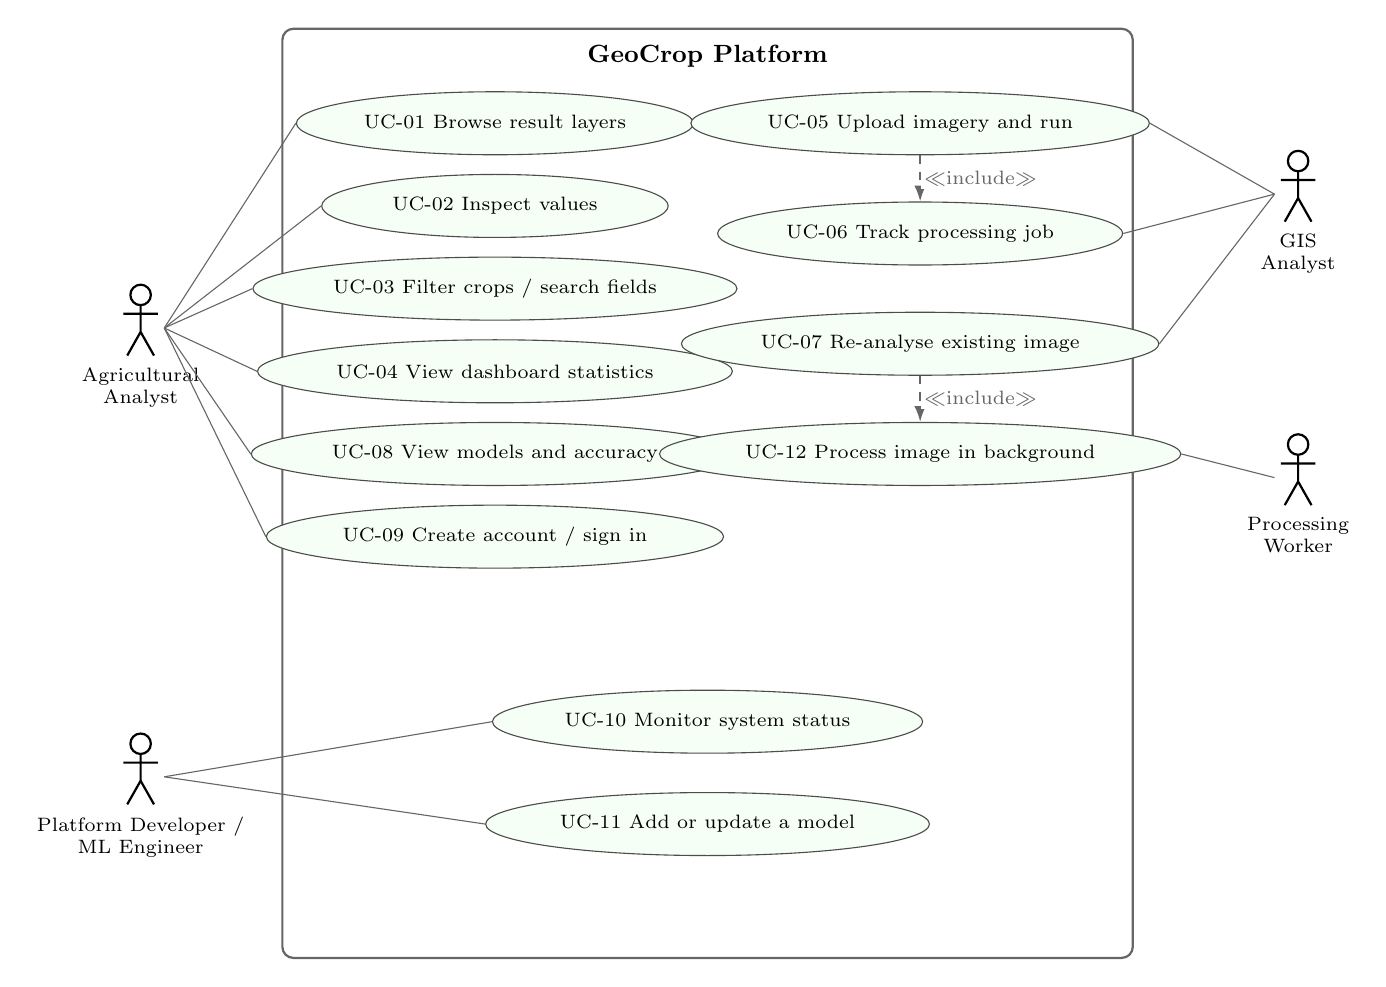
\begin{tikzpicture}[
  uc/.style={draw=black!70, ellipse, fill=green!4, minimum width=4.4cm, minimum height=0.8cm, font=\scriptsize, align=center},
  actor/.style={font=\scriptsize, align=center}]
\newcommand{\stick}[2]{%
  \begin{scope}[shift={(#1)}]
  \draw[thick] (0,0.42) circle (0.13);
  \draw[thick] (0,0.29) -- (0,-0.05) (-0.22,0.18) -- (0.22,0.18) (0,-0.05) -- (-0.17,-0.35) (0,-0.05) -- (0.17,-0.35);
  \node[actor, below] at (0,-0.38) {#2};
  \end{scope}}
\draw[rounded corners=4pt, thick, black!60] (-2.7,-6.3) rectangle (8.1,5.5);
\node[font=\small\bfseries] at (2.7,5.15) {GeoCrop Platform};
\node[uc] (u1) at (0,4.3) {UC-01 Browse result layers};
\node[uc] (u2) at (0,3.25) {UC-02 Inspect values};
\node[uc] (u3) at (0,2.2) {UC-03 Filter crops / search fields};
\node[uc] (u4) at (0,1.15) {UC-04 View dashboard statistics};
\node[uc] (u8) at (0,0.1) {UC-08 View models and accuracy};
\node[uc] (u9) at (0,-0.95) {UC-09 Create account / sign in};
\node[uc] (u5) at (5.4,4.3) {UC-05 Upload imagery and run};
\node[uc] (u6) at (5.4,2.9) {UC-06 Track processing job};
\node[uc] (u7) at (5.4,1.5) {UC-07 Re-analyse existing image};
\node[uc] (u12) at (5.4,0.1) {UC-12 Process image in background};
\node[uc] (u10) at (2.7,-3.3) {UC-10 Monitor system status};
\node[uc] (u11) at (2.7,-4.6) {UC-11 Add or update a model};
\stick{-4.5,1.7}{Agricultural\\Analyst}
\stick{10.2,3.4}{GIS\\Analyst}
\stick{-4.5,-4.0}{Platform Developer /\\ML Engineer}
\stick{10.2,-0.2}{Processing\\Worker}
\foreach \u in {u1,u2,u3,u4,u8,u9} \draw[black!60] (-4.2,1.7) -- (\u.west);
\foreach \u in {u5,u6,u7} \draw[black!60] (9.9,3.4) -- (\u.east);
\draw[black!60] (9.9,-0.2) -- (u12.east);
\draw[black!60] (-4.2,-4.0) -- (u10.west);
\draw[black!60] (-4.2,-4.0) -- (u11.west);
\draw[darr] (u5.south) -- node[lbl, right] {$\ll$include$\gg$} (u6.north);
\draw[darr] (u7.south) -- node[lbl, right] {$\ll$include$\gg$} (u12.north);
\end{tikzpicture}}
\caption{Use case diagram of the GeoCrop platform}
\label{fig:usecase}
\end{figure}

\section{Detailed Use Cases}
Three central use cases are given here; the remaining ones are in Appendix~\ref{app:requirements}.

\begin{table}[htbp]
\centering\small
\caption{Detailed use case UC-05: Upload imagery and run analysis}
\label{tab:uc05}
\begin{tabularx}{\textwidth}{L{3.0cm} Y}
\toprule
\textbf{Field} & \textbf{Description}\\
\midrule
Actor & GIS Analyst\\
Preconditions & Platform services are running; the user has access (sign-in optional in the current configuration).\\
Trigger & User opens Analyze Imagery.\\
Main flow & 1. User drops or selects a Sentinel-2 GeoTIFF and optionally enters location and capture date.\\
 & 2. User selects analysis models; dependencies (crop type needs cropland) are resolved automatically.\\
 & 3. System creates an upload record and returns a signed storage URL; the browser uploads the file directly to object storage.\\
 & 4. System creates a job with planned steps and queues ingestion; user is taken to the Processing page.\\
 & 5. Worker validates, reprojects to the model grid, converts to COG and publishes the image layer (UC-12).\\
 & 6. Worker runs the selected models in dependency order and publishes each result layer with statistics.\\
 & 7. User sees ``Analysis complete'' and opens the result on the Live Map.\\
Alternative flows & 1a. File is not a GeoTIFF: rejected before upload with a message. 5a. No coordinate system or wrong band count: job fails with a readable reason. 6a. A model is a placeholder: its step is skipped and marked as not available.\\
Postconditions & New area, image layer, result layers, statistics and job history are stored.\\
Related requirements & FR-ING-01 to FR-ING-07, FR-REG-03, NFR-P4\\
\bottomrule
\end{tabularx}
\end{table}

\begin{table}[htbp]
\centering\small
\caption{Detailed use case UC-01 / UC-02: Browse layers and inspect values}
\label{tab:uc01}
\begin{tabularx}{\textwidth}{L{3.0cm} Y}
\toprule
\textbf{Field} & \textbf{Description}\\
\midrule
Actor & Agricultural Analyst, GIS Analyst\\
Preconditions & At least one area with published layers exists.\\
Main flow & 1. User opens Live Map; the first area is selected and imagery and crop type are shown.\\
 & 2. User toggles layers in the Layer panel, changes opacity and reads legends.\\
 & 3. The map requests only the tiles in view; the Live map panel shows tiles loaded and latency.\\
 & 4. User clicks the map; the system returns the value and class label of every visible raster layer and the field region under the cursor.\\
Alternative flows & 2a. Area has no layers: an empty state explains how to create them. 4a. Point outside the data: ``No data''.\\
Postconditions & None (read-only).\\
Related requirements & FR-VIS-01 to FR-VIS-07, NFR-P1 to NFR-P3\\
\bottomrule
\end{tabularx}
\end{table}

\begin{table}[htbp]
\centering\small
\caption{Detailed use case UC-11: Add or update an analysis model}
\label{tab:uc11}
\begin{tabularx}{\textwidth}{L{3.0cm} Y}
\toprule
\textbf{Field} & \textbf{Description}\\
\midrule
Actor & Platform Developer / ML Engineer\\
Preconditions & Trained weights (if any) are available.\\
Main flow & 1. Developer copies the template model folder and edits \code{manifest.yaml} (key, name, requires, outputs, colour map).\\
 & 2. Developer implements \code{run()} in \code{task.py}: read the image, write a GeoTIFF, return it with class names and metrics.\\
 & 3. Weights are placed in the model artifact directory.\\
 & 4. API and worker are restarted; the registry discovers the model and stores it in the catalogue.\\
 & 5. The model appears on the Models page and in Analyze Imagery; its outputs become layers with legends and statistics.\\
Alternative flows & 4a. Invalid manifest: the error is shown on the Models and Status pages; other models keep working.\\
Related requirements & FR-REG-01 to FR-REG-05, NFR-R4\\
\bottomrule
\end{tabularx}
\end{table}

\section{Functional Requirements}
\subsection{Module 1: Processing Pipeline (Ingestion and Jobs)}
\begin{itemize}[leftmargin=2.2cm]
  \item[FR-ING-01] The system shall accept GeoTIFF uploads up to a configured size limit.
  \item[FR-ING-02] The system shall upload files directly to object storage through signed URLs,
        with an API fallback.
  \item[FR-ING-03] The system shall validate that an image is readable, georeferenced and has a
        supported band count, and report the reason when it is not.
  \item[FR-ING-04] The system shall reproject images to the model grid (EPSG:5070, 30~m) and convert
        them to Cloud Optimized GeoTIFF.
  \item[FR-ING-05] The system shall run analysis as background jobs and record per-step progress.
  \item[FR-ING-06] The system shall store optional location and capture date with an upload.
  \item[FR-ING-07] The system shall allow models to be re-run on an existing image.
\end{itemize}

\subsection{Module 2: Model Registry and Crop Mapping}
\begin{itemize}[leftmargin=2.2cm]
  \item[FR-REG-01] The system shall discover models from folders containing a manifest and a task.
  \item[FR-REG-02] The system shall list registered models with status, inputs, outputs, valid regions
        and stored accuracy.
  \item[FR-REG-03] The system shall resolve model dependencies and run them in order.
  \item[FR-REG-04] Placeholder models shall return ``not available'' and never produce data.
  \item[FR-REG-05] A model failure or invalid manifest shall not stop other models from loading.
  \item[FR-MAP-01] The system shall classify each pixel as cropland or non-cropland.
  \item[FR-MAP-02] The system shall classify the crop type of cropland pixels into the supported
        classes, grouping rare classes as ``Other''.
\end{itemize}

\subsection{Module 3: Catalogue, Storage and Statistics}
\begin{itemize}[leftmargin=2.2cm]
  \item[FR-CAT-01] The system shall store areas, images, runs, layers, statistics, field regions and
        jobs in a spatial database.
  \item[FR-CAT-02] The system shall compute area per class for each published categorical layer.
  \item[FR-CAT-03] The system shall derive field regions with area from crop-type output and publish
        them as vector tiles.
  \item[FR-CAT-04] Published files shall be immutable and versioned.
\end{itemize}

\subsection{Module 4: Web GIS Portal}
\begin{itemize}[leftmargin=2.2cm]
  \item[FR-VIS-01] The portal shall show a home page and navigation to Dashboard, Live Map, Analyze
        Imagery and Models.
  \item[FR-VIS-02] The Live Map shall build its layer panel from the catalogue, grouped by type, with
        toggles, opacity and legends.
  \item[FR-VIS-03] The Live Map shall render raster layers as XYZ tiles and vector layers as PMTiles.
  \item[FR-VIS-04] Clicking the map shall return values and labels of all visible layers.
  \item[FR-VIS-05] Users shall filter the map by crop and search field regions by crop.
  \item[FR-VIS-06] The portal shall switch between areas and between acres and hectares.
  \item[FR-VIS-07] The dashboard shall show area by class, shares and model accuracy.
  \item[FR-VIS-08] The portal shall show system health and configuration notes.
  \item[FR-AUT-01] Users shall be able to create an account and sign in; sign-in can be required by
        configuration.
\end{itemize}

\section{Non-Functional Requirements}
\subsection{Reliability}
\begin{itemize}[leftmargin=1.8cm]
  \item[NFR-R1] The whole stack shall start with one command and recover from start-up ordering
        (health-checked dependencies, retrying storage initialisation).
  \item[NFR-R2] Failed jobs shall record a readable error and leave existing data unchanged.
  \item[NFR-R3] Rebuilding one service shall not require restarting the others.
  \item[NFR-R4] One broken model shall not prevent other models from loading.
\end{itemize}
\subsection{Usability}
\begin{itemize}[leftmargin=1.8cm]
  \item[NFR-U1] Every layer shall have a legend with readable class names.
  \item[NFR-U2] Errors shall explain what went wrong and how to fix it.
  \item[NFR-U3] The interface shall work at phone and desktop widths without horizontal scrolling.
  \item[NFR-U4] Accuracy figures shall be shown with their evaluation protocol.
\end{itemize}
\subsection{Performance}
\begin{itemize}[leftmargin=1.8cm]
  \item[NFR-P1] One screen of an AOI shall need under 1~MB of map data.
  \item[NFR-P2] Cold tiles shall return in under 300~ms (median); cached tiles in under 50~ms.
  \item[NFR-P3] Eight or more layers shall be usable at once without visible lag.
  \item[NFR-P4] An AOI-sized image shall be processed by cropland and crop-type models in under
        2 minutes on a laptop CPU.
  \item[NFR-P5] The selected crop-type model shall run on CPU and be small (target: tens of MB or
        less).
\end{itemize}
\subsection{Security}
\begin{itemize}[leftmargin=1.8cm]
  \item[NFR-S1] Passwords shall be stored hashed (bcrypt); sessions use signed tokens.
  \item[NFR-S2] Secrets shall come from environment variables, not code.
  \item[NFR-S3] Users shall only see their own and public areas and layers.
  \item[NFR-S4] Upload URLs shall be short-lived and limited to one object.
  \item[NFR-S5] The tile service shall take styles from the server, not from request parameters.
\end{itemize}

\section{Acceptance Criteria}
\begin{table}[htbp]
\centering\small
\caption{Acceptance criteria for important requirements}
\label{tab:acceptance}
\begin{tabularx}{\textwidth}{L{2.2cm} Y L{2.2cm}}
\toprule
\textbf{Requirement} & \textbf{Acceptance check} & \textbf{Result}\\
\midrule
NFR-P1 & Benchmark: data for one screen of AOI1 at zoom 12 below 1~MB. & 337~KB, pass\\
NFR-P2 & Benchmark: cold tile median below 300~ms; cached below 50~ms. & 47~ms / 1~ms, pass\\
NFR-P4 & Upload AOI1 Sentinel-2 image, run both models, layers listed. & 57~s, pass\\
FR-REG-01 & Copy the template model, edit only the manifest; model loads and runs. & Pass (TC-03)\\
FR-REG-04 & Run yield placeholder; no files produced. & Pass (TC-04)\\
FR-ING-03 & Upload a 1-band file; job fails with a readable reason. & Pass (TC-13)\\
FR-VIS-04 & Click a pivot field; crop type and cropland labels returned. & Pass (TC-08)\\
FR-VIS-05 & Filter ``Apples''; only apple pixels remain on the map. & Pass (TC-09)\\
NFR-R1 & \code{docker compose down} then \code{up -d}; health OK for all services. & Pass (TC-15)\\
FR-MAP-02 & Crop-type accuracy and macro-F1 on spatial test blocks reported with intervals. & 76.1\% / 92.2\%, reported\\
\bottomrule
\end{tabularx}
\end{table}

\section{Requirements Traceability}
\begin{table}[htbp]
\centering\small
\caption{Traceability of key requirements to modules, design, implementation and tests}
\label{tab:trace}
\begin{tabularx}{\textwidth}{L{1.9cm} L{1.3cm} L{3.4cm} Y L{1.4cm}}
\toprule
\textbf{Req.} & \textbf{Module} & \textbf{Design element} & \textbf{Implementation} & \textbf{Test}\\
\midrule
FR-ING-02 & M5 & Signed upload (Fig.~\ref{fig:seq}) & \code{routes.py: create_upload}, \code{storage.py} & TC-11\\
FR-ING-03/04 & M5, M1 & Ingest task & \code{tasks.py: ingest_upload}, \code{rasters.py} & TC-11, TC-13\\
FR-ING-05 & M5 & Job states (Fig.~\ref{fig:states}) & \code{tasks.py: run_pipeline}, \code{Job} & TC-11, TC-12\\
FR-REG-01/03 & M6 & Registry, graph & \code{registry.py}, \code{graph.py} & TC-01, TC-02, TC-03\\
FR-REG-04 & M6 & StubTask & \code{base.py: StubTask} & TC-04\\
FR-MAP-01/02 & M2 & Model tasks & \code{builtin/cropland}, \code{builtin/croptype} & TC-11, Ch.~\ref{ch:iter1}\\
FR-CAT-02 & M7 & ZonalStat & \code{rasters.py: categorical_stats} & TC-07\\
FR-CAT-03 & M3 & PMTiles layer & \code{vector_tiles.py} & TC-10\\
FR-VIS-03 & M8 & Tile service & \code{tiles/main.py}, \code{LiveMap.tsx} & TC-05, TC-06\\
FR-VIS-04 & M8 & Point query & \code{routes.py: point} & TC-08\\
FR-VIS-05 & M8 & Crop filter & \code{tiles/main.py: classes}, \code{LiveMap.tsx} & TC-09\\
NFR-P1/P2 & M8 & Tiles, cache & \code{nginx.conf}, \code{benchmark_tiles.py} & TC-14\\
NFR-R1 & -- & Compose health checks & \code{docker-compose.yml}, \code{minio-init.sh} & TC-15\\
\bottomrule
\end{tabularx}
\end{table}

\chapter{System Design}

\section{System Architecture}
GeoCrop follows a layered, service-oriented architecture built around one principle: \emph{send
only what is visible}. Model results are stored once as Cloud Optimized GeoTIFFs (COG) in object
storage; the browser requests small map tiles for the current view, which a stateless tile service
cuts from the COG and Nginx caches. Heavy work runs in background workers, and a spatial database
holds the catalogue that tells the interface what exists. The main building blocks are the COG
format~\cite{cog}, TiTiler~\cite{titiler}, PMTiles~\cite{pmtiles}, MapLibre GL~\cite{maplibre} and
PostGIS~\cite{postgis}. Figure~\ref{fig:arch} shows the services
and their connections.

\begin{figure}[htbp]
\centering
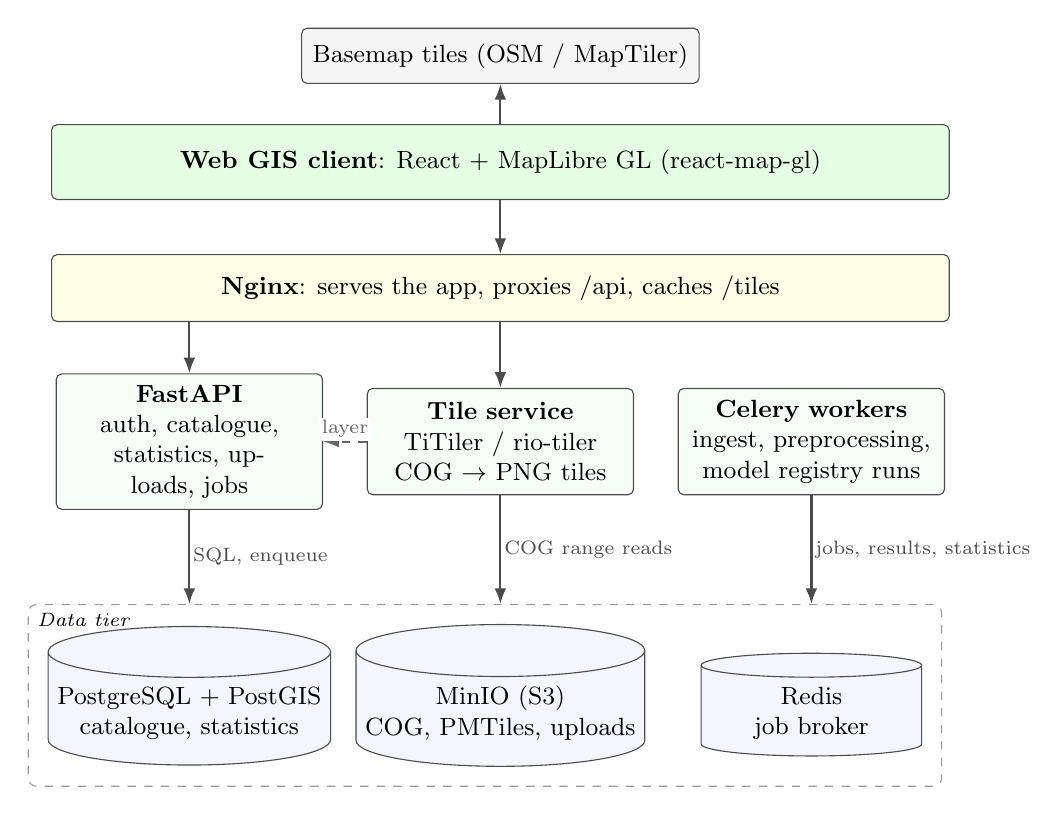
\begin{tikzpicture}[every node/.style={font=\small}]
\node[box, minimum width=4.2cm, minimum height=0.7cm, fill=gray!8] (base) at (0,1.35) {Basemap tiles (OSM / MapTiler)};
\node[box, minimum width=11.4cm, minimum height=0.95cm, fill=green!10] (client) at (0,0) {\textbf{Web GIS client}: React + MapLibre GL (react-map-gl)};
\node[box, minimum width=11.4cm, minimum height=0.85cm, fill=yellow!10] (nginx) at (0,-1.6) {\textbf{Nginx}: serves the app, proxies /api, caches /tiles};
\node[box, text width=3.1cm, minimum height=1.35cm] (api) at (-3.95,-3.55) {\textbf{FastAPI}\\auth, catalogue, statistics, uploads, jobs};
\node[box, text width=3.1cm, minimum height=1.35cm] (tiles) at (0,-3.55) {\textbf{Tile service}\\TiTiler / rio-tiler\\COG $\rightarrow$ PNG tiles};
\node[box, text width=3.1cm, minimum height=1.35cm] (worker) at (3.95,-3.55) {\textbf{Celery workers}\\ingest, preprocessing, model registry runs};
\node[dbox, minimum width=2.8cm] (pg) at (-3.95,-7.0) {PostgreSQL + PostGIS\\catalogue, statistics};
\node[dbox, minimum width=2.8cm] (s3) at (0,-7.0) {MinIO (S3)\\COG, PMTiles, uploads};
\node[dbox, minimum width=2.8cm] (redis) at (3.95,-7.0) {Redis\\job broker};
\node[lane, fit=(pg)(s3)(redis), inner sep=7pt, label={[font=\scriptsize\itshape, anchor=north west]north west:Data tier}] (data) {};
\draw[arr] (client) -- (base);
\draw[arr] (client) -- (nginx);
\draw[arr] (nginx.south -| api.north) -- (api.north);
\draw[arr] (nginx.south -| tiles.north) -- (tiles.north);
\draw[darr] (tiles.west) -- node[lbl,above]{layer} (api.east);
\draw[arr] (api.south) -- node[lbl,right]{SQL, enqueue} (api.south |- data.north);
\draw[arr] (tiles.south) -- node[lbl,right]{COG range reads} (tiles.south |- data.north);
\draw[arr] (worker.south) -- node[lbl,right]{jobs, results, statistics} (worker.south |- data.north);
\end{tikzpicture}
\caption{GeoCrop system architecture. The browser also reads PMTiles and uploads imagery directly to object storage using short-lived signed URLs; the tile service looks up layer styles from the API.}
\label{fig:arch}
\end{figure}

\section{Architectural Components}
\begin{table}[htbp]
\centering\small
\caption{Architectural components}
\label{tab:components}
\begin{tabularx}{\textwidth}{L{3.0cm} L{3.4cm} Y}
\toprule
\textbf{Component} & \textbf{Technology} & \textbf{Responsibility}\\
\midrule
Web GIS client & React, Vite, TypeScript, MapLibre GL via react-map-gl, TanStack Query, Zustand & Home, Live Map workspace, Dashboard, Analyze Imagery, Processing, Models, Status, accounts. Builds layers from the catalogue; loads tiles on demand.\\
Edge & Nginx & Serves the built app; proxies the API; caches tiles with immutable headers; resolves services through Docker DNS at request time.\\
API service & FastAPI, Pydantic, SQLAlchemy 2, GeoAlchemy2, PyJWT, bcrypt & REST API v1: health, auth, areas, models, layers, fields, point query, statistics, uploads, runs, jobs.\\
Tile service & TiTiler / rio-tiler (FastAPI) & \code{/tiles/{layer}/{version}/{z}/{x}/{y}.png}; reads only needed COG blocks; applies the server-side style; optional crop filter.\\
Workers & Celery & Ingest (validate, reproject, COG), model runs through the registry, statistics, layer publishing, progress.\\
Model registry & Python package with YAML manifests & Discovers models, resolves dependencies, runs tasks with a common context; built-in cropland, crop type, NDVI index, boundary and yield placeholders.\\
Spatial database & PostgreSQL 16 + PostGIS 3.4, Alembic & Catalogue of users, areas, uploads, images, models, runs, layers, statistics, field regions, jobs.\\
Job broker & Redis 7 & Celery broker and result backend.\\
Object storage & MinIO (S3 API) & Uploads, COG imagery and results, PMTiles; anonymous read only for vector tiles.\\
\bottomrule
\end{tabularx}
\end{table}

\section{Interfaces and Dependencies}
\begin{table}[htbp]
\centering\small
\caption[Main REST interfaces]{Main REST interfaces (prefix \code{/api/v1}; interactive documentation at \code{/api/docs})}
\label{tab:api}
\begin{tabularx}{\textwidth}{L{5.2cm} Y}
\toprule
\textbf{Endpoint} & \textbf{Purpose}\\
\midrule
\code{GET /health} & Status of database, broker, storage, tiles and model registry; configuration notes.\\
\code{POST /auth/signup}, \code{/auth/login}, \code{GET /auth/me} & Accounts and tokens.\\
\code{GET /aois} & Areas visible to the user, with bounds.\\
\code{GET /models} & Registered models, status, inputs, outputs, accuracy and per-class scores.\\
\code{GET /layers?aoi=&kind=&run=} & Layer catalogue: style, legend, bounds, zoom range, tile URL, version.\\
\code{GET /fields?aoi=&q=} & Field regions with crop, area and bounding box.\\
\code{GET /point?lng=&lat=&layers=} & Values and labels of several layers at one location.\\
\code{GET /stats?layer=} & Pre-computed area and share per class.\\
\code{POST /uploads}, \code{/uploads/{id}/complete} & Signed upload URL; start ingestion with models, location and date.\\
\code{POST /runs}, \code{GET /runs}, \code{GET /jobs/{id}} & Re-run models; run history; job progress and steps.\\
\code{GET /tiles/{layer}/{v}/{z}/{x}/{y}.png} & Raster tiles (tile service, cached by Nginx).\\
\bottomrule
\end{tabularx}
\end{table}
External dependencies are Sentinel-2 imagery exported with Google Earth Engine, USDA CDL rasters and
AOI shapefiles, an OpenStreetMap or MapTiler basemap, and the open-source libraries listed in
Section~\ref{sec:external}. Internally, the API depends on the database, broker and storage; the tile
service depends on the API (layer lookup, cached for five minutes) and storage; workers depend on the
broker, database, storage and model artifacts.

\section{Architecture Decisions and Rationale}
\begin{table}[htbp]
\centering\small
\caption{Key architecture decisions}
\label{tab:adr}
\begin{tabularx}{\textwidth}{L{3.6cm} Y L{3.6cm}}
\toprule
\textbf{Decision} & \textbf{Rationale} & \textbf{Alternative rejected}\\
\midrule
Raster as source of truth (COG) & Models predict pixels; a 30~m raster of AOI1 is about 1.6~MB, the same result as polygons 43.3~MB. & Vectorising all output to GeoJSON\\
Tiles via TiTiler & Reads only the COG blocks needed per tile; styles applied on the server; no pre-rendering. & Pre-rendered tile folders; single PNG overlays\\
PMTiles for vectors & One static file read by range requests; no tile server; cacheable. & GeoJSON; dynamic vector tile server\\
MapLibre GL & WebGL rendering of raster and vector tiles; open source. & Leaflet (SVG/Canvas)\\
Versioned, immutable tile URLs & Browsers and Nginx can cache for a year; a new run gets a new URL. & Cache invalidation logic\\
FastAPI & Same stack as TiTiler; async I/O; typed schemas and generated docs. & Django templates (prototype)\\
PostgreSQL + PostGIS & Spatial types and indexes, joins between catalogue and statistics, JSONB for styles and metrics. & SQLite (prototype)\\
Celery + Redis & Long jobs off the request path; retries; progress. & Synchronous processing\\
S3-compatible storage (MinIO) & Large files, range reads, signed uploads, cloud-portable. & Local disk\\
Manifest-based model registry & Models change over the project; new models without changes elsewhere. & Hard-coded model calls\\
Docker Compose & One-command, reproducible stack for the team and the panel. & Manual installation\\
\bottomrule
\end{tabularx}
\end{table}

\section{Design Evolution}\label{sec:evolution}
The proposal-stage prototype was a Django application with Leaflet. It returned the crop-type result
for AOI1 as one GeoJSON response; the browser parsed it and drew 101,435 polygons as SVG. Uploads
were recorded but never processed, field data on the dashboard was hand-written, and the session
cookie held upload history. Table~\ref{tab:evolution} summarises the changes and why they were made.

\begin{table}[htbp]
\centering\small
\caption{Design evolution since the proposal}
\label{tab:evolution}
\begin{tabularx}{\textwidth}{L{2.6cm} L{3.6cm} L{4.0cm} Y}
\toprule
\textbf{Aspect} & \textbf{Proposal prototype} & \textbf{Current design} & \textbf{Reason}\\
\midrule
Result format & GeoJSON polygons (43.3~MB) & COG rasters + PMTiles & Data volume and rendering cost\\
Map client & Leaflet, SVG & MapLibre GL, WebGL tiles & Smooth zoom with many layers\\
Backend & Django views and templates & FastAPI + React SPA & Async API, typed contracts, separation of concerns\\
Database & SQLite & PostgreSQL + PostGIS & Spatial queries, concurrency, catalogue\\
Processing & None (upload recorded only) & Celery jobs with progress & Real analysis of new imagery\\
Models & Offline scripts writing GeoJSON & Registry plug-ins writing rasters & Add models without code changes\\
Dashboard data & Hard-coded sample fields & Pre-computed statistics in PostGIS & Real results\\
Deployment & Single process & Seven containers via Compose & Reproducible, scalable services\\
\bottomrule
\end{tabularx}
\end{table}

\section{Domain Model}
Figure~\ref{fig:domain} shows the main domain classes. An \emph{Area of Interest} owns source images
and model runs; a run executes one registered \emph{Model} and produces one or more \emph{Layers};
categorical layers are summarised by \emph{Zonal statistics}; crop-type runs also produce
\emph{Field regions}. A \emph{Job} tracks the steps of an upload or a run.

\begin{figure}[htbp]
\centering
\resizebox{\textwidth}{!}{%
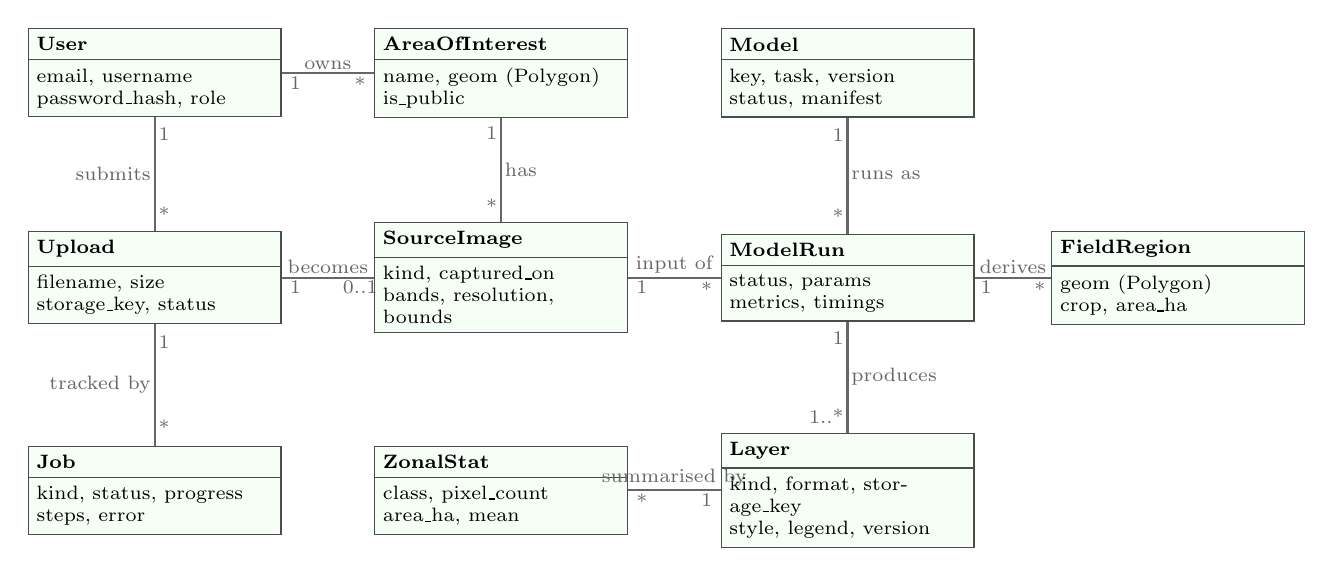
\begin{tikzpicture}[
  cls/.style={draw=black!70, rectangle split, rectangle split parts=2, fill=green!4, font=\scriptsize, align=left, text width=3.0cm, inner sep=3pt, rectangle split part fill={green!14,green!3}},
  rel/.style={thick, black!60}, m/.style={font=\scriptsize, inner sep=1pt}]
\node[cls] (user) at (0,0) {\textbf{User}\nodepart{second}email, username\\password\_hash, role};
\node[cls] (aoi) at (4.4,0) {\textbf{AreaOfInterest}\nodepart{second}name, geom (Polygon)\\is\_public};
\node[cls] (upload) at (0,-2.6) {\textbf{Upload}\nodepart{second}filename, size\\storage\_key, status};
\node[cls] (img) at (4.4,-2.6) {\textbf{SourceImage}\nodepart{second}kind, captured\_on\\bands, resolution, bounds};
\node[cls] (model) at (8.8,0) {\textbf{Model}\nodepart{second}key, task, version\\status, manifest};
\node[cls] (run) at (8.8,-2.6) {\textbf{ModelRun}\nodepart{second}status, params\\metrics, timings};
\node[cls] (layer) at (8.8,-5.3) {\textbf{Layer}\nodepart{second}kind, format, storage\_key\\style, legend, version};
\node[cls] (stat) at (4.4,-5.3) {\textbf{ZonalStat}\nodepart{second}class, pixel\_count\\area\_ha, mean};
\node[cls] (field) at (13.0,-2.6) {\textbf{FieldRegion}\nodepart{second}geom (Polygon)\\crop, area\_ha};
\node[cls] (job) at (0,-5.3) {\textbf{Job}\nodepart{second}kind, status, progress\\steps, error};
\draw[rel] (user) -- node[m,above]{owns} node[m,pos=0.15,below]{1} node[m,pos=0.85,below]{*} (aoi);
\draw[rel] (user) -- node[m,left]{submits} node[m,pos=0.15,right]{1} node[m,pos=0.85,right]{*} (upload);
\draw[rel] (upload) -- node[m,above]{becomes} node[m,pos=0.15,below]{1} node[m,pos=0.85,below]{0..1} (img);
\draw[rel] (aoi) -- node[m,right]{has} node[m,pos=0.15,left]{1} node[m,pos=0.85,left]{*} (img);
\draw[rel] (model) -- node[m,right]{runs as} node[m,pos=0.15,left]{1} node[m,pos=0.85,left]{*} (run);
\draw[rel] (img) -- node[m,above]{input of} node[m,pos=0.15,below]{1} node[m,pos=0.85,below]{*} (run);
\draw[rel] (run) -- node[m,right]{produces} node[m,pos=0.15,left]{1} node[m,pos=0.85,left]{1..*} (layer);
\draw[rel] (layer) -- node[m,above]{summarised by} node[m,pos=0.15,below]{1} node[m,pos=0.85,below]{*} (stat);
\draw[rel] (run) -- node[m,above]{derives} node[m,pos=0.15,below]{1} node[m,pos=0.85,below]{*} (field);
\draw[rel] (upload) -- node[m,left]{tracked by} node[m,pos=0.15,right]{1} node[m,pos=0.85,right]{*} (job);
\end{tikzpicture}}
\caption{Domain model}
\label{fig:domain}
\end{figure}

\section{Data Design}
\textbf{Relational schema.} The catalogue is a PostgreSQL/PostGIS schema managed with Alembic
(Table~\ref{tab:schema}). Geometries are stored in EPSG:4326 with GiST spatial indexes. Free-form
fields (layer kind, style, legend, model manifest, run metrics) are strings or JSONB, so a new model
output never needs a schema change. Rasters are never stored in the database.

\begin{table}[htbp]
\centering\small
\caption{Database tables}
\label{tab:schema}
\begin{tabularx}{\textwidth}{L{2.4cm} Y}
\toprule
\textbf{Table} & \textbf{Key columns}\\
\midrule
\code{users} & id, email (unique), username (unique), password\_hash, role, created\_at\\
\code{aoi} & id, owner\_id, name, geom (Polygon, GiST), is\_public\\
\code{upload} & id, user\_id, aoi\_id, filename, size\_bytes, storage\_key, status\\
\code{source_image} & id, aoi\_id, upload\_id, kind, captured\_on, storage\_key, bounds (GiST), band\_count, resolution\_m\\
\code{model} & id, key (unique), task, version, name, status, manifest (JSONB), enabled\\
\code{model_run} & id, aoi\_id, model\_id, source\_image\_id, status, params, metrics (JSONB), error, timings\\
\code{map_layer} & id, run\_id, aoi\_id, kind, group, name, format, storage\_key, bounds (GiST), zoom range, nodata, style, legend (JSONB), version, is\_public\\
\code{zonal_stat} & layer\_id, zone\_type, zone\_id, class\_code, class\_name, pixel\_count, area\_ha, mean, min, max\\
\code{field} & id, aoi\_id, run\_id, geom (Polygon, GiST), attributes (JSONB)\\
\code{job} & id, kind, status, progress, message, error, steps (JSONB), upload\_id, user\_id\\
\bottomrule
\end{tabularx}
\end{table}

\textbf{Object storage layout} (bucket \code{geocrop}): \code{raw/{upload}/original.tif} for
uploads; \code{runs/reference/...cog.tif} for imagery and reference layers;
\code{runs/{run}/{kind}-{id}.cog.tif} for model outputs; and \code{vector/{aoi}/{run}/...pmtiles}
for vector layers. Files are written once; a new run creates new keys.

\textbf{Raster conventions.} COGs use 512-pixel internal blocks, DEFLATE compression and overviews
(nearest neighbour for class maps, average for imagery). Categorical rasters use 0 as no-data; the
cropland map uses 1 = cropland and 2 = non-cropland; crop-type codes map to class names stored in the
layer legend.

\section{Process / Behavior Design}
\textbf{Upload to map.} Figure~\ref{fig:seq} shows the interaction from upload to published layers.

\begin{figure}[htbp]
\centering
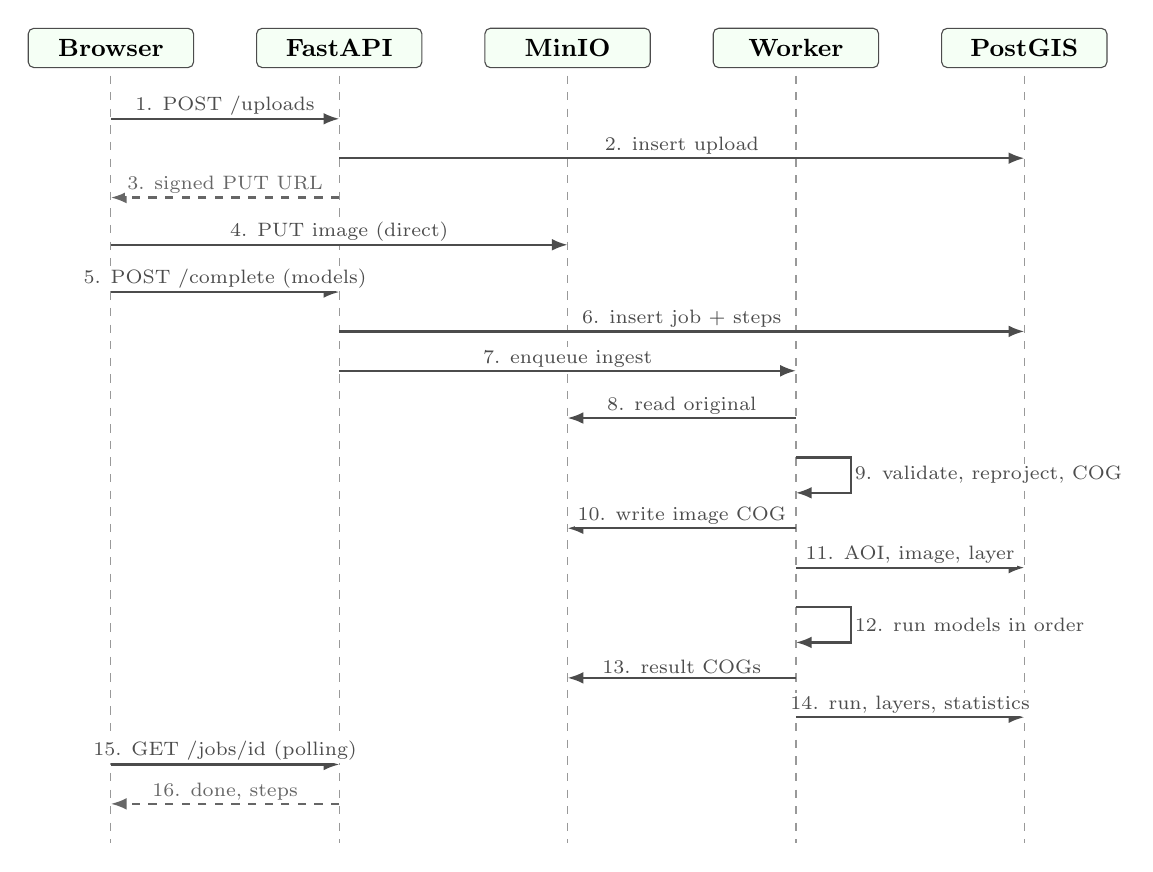
\begin{tikzpicture}[font=\scriptsize]
\foreach \x/\n/\t in {0/b/Browser, 2.9/a/FastAPI, 5.8/s/MinIO, 8.7/w/Worker, 11.6/d/PostGIS}{
  \node[box, minimum width=2.1cm] (\n) at (\x,0) {\textbf{\t}};
  \draw[dashed, black!40] (\x,-0.35) -- (\x,-10.1);
}
\newcommand{\msg}[5]{\draw[#5] (#1,#3) -- node[lbl,above]{#4} (#2,#3);}
\msg{0}{2.9}{-0.9}{1. POST /uploads}{arr}
\msg{2.9}{11.6}{-1.4}{2. insert upload}{arr}
\msg{2.9}{0}{-1.9}{3. signed PUT URL}{darr}
\msg{0}{5.8}{-2.5}{4. PUT image (direct)}{arr}
\msg{0}{2.9}{-3.1}{5. POST /complete (models)}{arr}
\msg{2.9}{11.6}{-3.6}{6. insert job + steps}{arr}
\msg{2.9}{8.7}{-4.1}{7. enqueue ingest}{arr}
\msg{8.7}{5.8}{-4.7}{8. read original}{arr}
\draw[arr] (8.7,-5.2) -- ++(0.7,0) -- node[lbl,right]{9. validate, reproject, COG} ++(0,-0.45) -- ++(-0.7,0);
\msg{8.7}{5.8}{-6.1}{10. write image COG}{arr}
\msg{8.7}{11.6}{-6.6}{11. AOI, image, layer}{arr}
\draw[arr] (8.7,-7.1) -- ++(0.7,0) -- node[lbl,right]{12. run models in order} ++(0,-0.45) -- ++(-0.7,0);
\msg{8.7}{5.8}{-8.0}{13. result COGs}{arr}
\msg{8.7}{11.6}{-8.5}{14. run, layers, statistics}{arr}
\msg{0}{2.9}{-9.1}{15. GET /jobs/{id} (polling)}{arr}
\msg{2.9}{0}{-9.6}{16. done, steps}{darr}
\end{tikzpicture}
\caption{Sequence of an upload and analysis}
\label{fig:seq}
\end{figure}

\textbf{Job and run states.} A job moves from \emph{queued} to \emph{running} and ends in \emph{done}
or \emph{failed}; each step inside it is \emph{pending}, \emph{running}, \emph{done}, \emph{skipped}
(placeholder model) or \emph{failed} (Figure~\ref{fig:states}).

\begin{figure}[htbp]
\centering
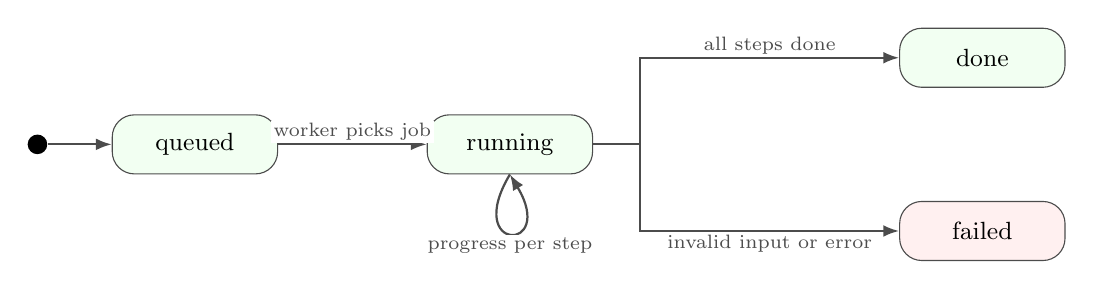
\begin{tikzpicture}[st/.style={draw=black!70, rounded corners=8pt, fill=green!5, minimum width=2.1cm, minimum height=0.75cm, font=\small}]
\node[circle, fill=black, inner sep=2.5pt] (start) at (0,0) {};
\node[st] (q) at (2,0) {queued};
\node[st] (r) at (6,0) {running};
\node[st] (d) at (12,1.1) {done};
\node[st, fill=red!6] (f) at (12,-1.1) {failed};
\draw[arr] (start) -- (q);
\draw[arr] (q) -- node[lbl,above]{worker picks job} (r);
\draw[arr] (r.east) -- ++(0.6,0) |- node[lbl,pos=0.75,above]{all steps done} (d.west);
\draw[arr] (r.east) -- ++(0.6,0) |- node[lbl,pos=0.75,below]{invalid input or error} (f.west);
\draw[arr] (r.south) .. controls +(-0.6,-1.0) and +(0.6,-1.0) .. node[lbl,below]{progress per step} (r.south);
\end{tikzpicture}
\caption{Job state machine}
\label{fig:states}
\end{figure}

\textbf{Model execution.} The registry plans the requested models with a topological sort over the
layer kinds they require and produce (for example, crop type requires cropland). Each model receives
a run context (image path, upstream outputs, scratch folder, artifacts, progress callback); its
output files are converted to COG, uploaded, registered as layers with style and legend, and
summarised as zonal statistics before the next model starts, so the map fills in progressively.

\textbf{Tile request.} The client requests \code{/tiles/{layer}/{version}/{z}/{x}/{y}.png}. Nginx
returns a cached copy when it has one; otherwise the tile service looks up the layer (cached),
reads the needed COG window from storage with nearest-neighbour resampling for class maps, applies
the stored colour map and returns a PNG with a one-year immutable cache header. Tiles outside the
raster return HTTP~204.

\chapter{Iteration 1: Design and Implementation}\label{ch:iter1}

\section{Iteration Objectives}
\begin{enumerate}
  \item \textbf{Architecture track:} design and implement a base architecture that keeps the map
        fast as images, models and layers grow, and prove it on the real AOI1 data.
  \item \textbf{Architecture track:} turn the prototype's ``upload and nothing happens'' into a real
        pipeline in which an uploaded image is analysed and published automatically.
  \item \textbf{Architecture track:} make models replaceable, so research results can be integrated
        without redesign.
  \item \textbf{Model track:} evaluate crop-type models under a fair spatial test, measure their cost,
        improve the best candidates, and compare with published work.
\end{enumerate}

\section{Selected Use Cases / Features}
\begin{table}[htbp]
\centering\small
\caption{Use cases and features selected for Iteration 1}
\label{tab:it1features}
\begin{tabularx}{\textwidth}{L{1.4cm} Y L{2.2cm}}
\toprule
\textbf{Use case} & \textbf{Feature} & \textbf{Track}\\
\midrule
UC-01, UC-02 & Tile-based Live Map with layer panel, legends, opacity, point inspection & Architecture\\
UC-03 & Crop filter, crop ranking and searchable field list & Architecture\\
UC-04 & Dashboard with pre-computed statistics and model accuracy & Architecture\\
UC-05, UC-06, UC-12 & Upload, background processing, live progress & Architecture\\
UC-07 & Re-analyse an existing image & Architecture\\
UC-08, UC-11 & Model catalogue and plug-in registry & Architecture\\
UC-09, UC-10 & Accounts and system status & Architecture\\
FR-MAP-02 & Crop-type model comparison, selection and error analysis & Model\\
\bottomrule
\end{tabularx}
\end{table}

\section{Design}
The architecture track implements the design of Chapter~5: Figure~\ref{fig:arch} (services),
Figure~\ref{fig:seq} (processing), Figure~\ref{fig:domain} and Table~\ref{tab:schema} (data). The
model track follows the experiment design in Figure~\ref{fig:experiment}: every experiment uses the
same inputs, split, classes and seed, and only the validation set decides.

\begin{figure}[htbp]
\centering
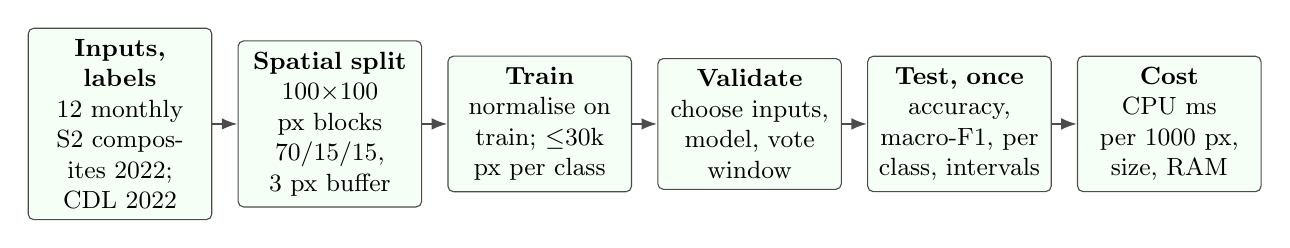
\begin{tikzpicture}[node distance=0.32cm, every node/.style={font=\scriptsize}]
\node[box, text width=2.05cm] (a) {\textbf{Inputs, labels}\\12 monthly S2 composites 2022; CDL 2022};
\node[box, text width=2.05cm, right=of a] (b) {\textbf{Spatial split}\\100$\times$100 px blocks 70/15/15, 3 px buffer};
\node[box, text width=2.05cm, right=of b] (c) {\textbf{Train}\\normalise on train; $\leq$30k px per class};
\node[box, text width=2.05cm, right=of c] (d) {\textbf{Validate}\\choose inputs, model, vote window};
\node[box, text width=2.05cm, right=of d] (e) {\textbf{Test, once}\\accuracy, macro-F1, per class, intervals};
\node[box, text width=2.05cm, right=of e] (f) {\textbf{Cost}\\CPU ms per 1000 px, size, RAM};
\draw[arr] (a)--(b); \draw[arr] (b)--(c); \draw[arr] (c)--(d); \draw[arr] (d)--(e); \draw[arr] (e)--(f);
\end{tikzpicture}
\caption{Crop-type experiment design}
\label{fig:experiment}
\end{figure}

\section{Implementation}
\textbf{Architecture track.} The platform was implemented as a new repository
(\code{geocrop-platform}) and runs as seven containers with Docker Compose: \code{web} (Nginx with
the built React app), \code{api} (FastAPI), \code{worker} (Celery), \code{tiles} (TiTiler),
\code{postgres} (PostGIS), \code{redis} and \code{minio}, plus a one-shot bucket initialiser.
Table~\ref{tab:loc} gives the size of each part. Data preparation scripts convert the AOI rasters to
COG, build the field-region PMTiles and load the AOI1 demonstration data.

\begin{table}[htbp]
\centering\small
\caption{Platform code by component (lines, including configuration and documentation)}
\label{tab:loc}
\begin{tabular}{L{4.0cm} L{6.6cm} r}
\toprule
\textbf{Component} & \textbf{Contents} & \textbf{Lines}\\
\midrule
\code{web/src} & React pages, map workspace, components, styles & 1,998\\
\code{backend/app} & API routes, models, services, workers, seed & 1,547\\
\code{backend/model_registry} & Contract, registry, graph, colour maps, models & 498\\
\code{ml} & Extended training scripts & 373\\
\code{docs} & Architecture, status, upgrade path, guides & 282\\
\code{tools} & COG conversion, boundaries, benchmark & 222\\
\code{tiles} & Tile service & 77\\
\code{infra} & Nginx and storage initialisation & 68\\
\bottomrule
\end{tabular}
\end{table}

\textbf{Model track.} Two notebooks implement the experiments: a benchmark notebook (runs 1 and 2,
model families, cost measurement, spatial bootstrap) and an accuracy-improvement notebook (run 3,
for AOI1 or AOI2). Inputs are 12 monthly Sentinel-2 composites of 2022 with 11 values per month
(B2, B3, B4, B5, B6, B7, B8, B8A, B11, B12 and NDVI) and the CDL 2022 rasters, all on the same 30~m
EPSG:5070 grid. AOI1 (eastern Washington, about 40$\times$37~km, 14 classes, 99,238 test pixels) is a
hard area with small fragmented fields, orchards and similar hay crops; AOI2 (north-eastern North
Dakota, about 38$\times$29~km, 9 classes, 144,922 test pixels) has large regular fields and two
dominant crops.

\section{Completed Features / Module}
\begin{table}[htbp]
\centering\small
\caption{Completed features at mid-term}
\label{tab:completed}
\begin{tabularx}{\textwidth}{L{3.8cm} Y L{1.4cm}}
\toprule
\textbf{Module} & \textbf{Completed} & \textbf{State}\\
\midrule
M1 Data preparation & COG conversion with validation; AOI1 Sentinel-2 composite and CDL as COG; monthly 2022 composites for AOI1 and AOI2 & Done\\
M2 Crop mapping & Platform: cropland and crop-type Random Forests trained and run on uploads. Research: 11 models compared; improved LightGBM pipeline selected & Done\\
M3 Field regions & 2,433 field regions (at least 25 pixels) as a 1.86~MB PMTiles layer and PostGIS rows & Interim\\
M4 Yield & Registered placeholder; NASS download script prepared & Planned\\
M5 Processing pipeline & Signed uploads, validation, reprojection, COG, background runs, progress, re-runs & Done\\
M6 Model registry & Contract, manifests, dependency graph, placeholders, NDVI template, add-a-model test & Done\\
M7 Catalogue and statistics & PostGIS schema with Alembic migration; zonal statistics; field search & Done\\
M8 Web GIS portal & Home, Live Map workspace, Dashboard, Analyze Imagery, Processing, Models, Status, accounts & Done\\
\bottomrule
\end{tabularx}
\end{table}

\section{Technical Implementation Details}
\begin{table}[htbp]
\centering\small
\caption{Important files, classes and functions}
\label{tab:files}
\begin{tabularx}{\textwidth}{L{5.3cm} Y}
\toprule
\textbf{File / element} & \textbf{Role}\\
\midrule
\code{model_registry/base.py}: \code{ModelTask}, \code{RunContext}, \code{RunResult}, \code{StubTask} & Contract every model implements; placeholders never fabricate data.\\
\code{model_registry/registry.py}: \code{Registry} & Scans folders for \code{manifest.yaml}, imports the entrypoint, isolates broken models.\\
\code{model_registry/graph.py}: \code{execution_order} & Topological order from required and produced layer kinds; readable errors for cycles and missing producers.\\
\code{builtin/cropland}, \code{builtin/croptype} & Windowed (512-pixel block) inference with saved models; crop type runs only on cropland pixels.\\
\code{app/workers/tasks.py}: \code{ingest_upload}, \code{run_pipeline} & Validate, reproject, convert, publish image; run models; publish layers and statistics; update job steps.\\
\code{app/services/layers.py}: \code{publish_raster_layer} & COG conversion, upload, footprint, layer row and zonal statistics in one step.\\
\code{app/services/rasters.py} & Footprint, point sampling, block-wise class statistics, reprojection to the model grid.\\
\code{app/services/vector_tiles.py} & Polygonise class rasters, simplify per zoom, encode MVT, write PMTiles.\\
\code{app/services/storage.py} & One storage interface for S3/MinIO and local disk; GDAL \code{/vsis3/} access.\\
\code{tiles/main.py} & Tile endpoint with server-side styles, crop filter, immutable caching.\\
\code{web/src/pages/LiveMap.tsx} & Map workspace; layers from the catalogue; filter, field search, inspection, tile traffic panel.\\
\code{docker-compose.yml}, \code{web/nginx.conf} & Services, health checks, tile cache, runtime DNS resolution.\\
\bottomrule
\end{tabularx}
\end{table}

Configuration is read from environment variables (\code{.env}); the database schema is created by an
Alembic migration that manages only GeoCrop's tables (the PostGIS image ships its own topology and
geocoder tables, which are excluded).

\section{Algorithms and Technical Decisions}
\subsection{Platform algorithms}
\begin{itemize}
  \item \textbf{COG conversion:} GDAL COG driver, 512-pixel blocks, DEFLATE, overviews with nearest
        neighbour for categorical rasters and average for imagery; validated by layout, tiling,
        overviews and CRS.
  \item \textbf{Tile rendering:} for tile $(z,x,y)$ the service reads the overlapping COG window at
        the matching overview, resamples (nearest for classes), maps class codes to the stored
        colours (optionally only selected classes) and encodes a PNG.
  \item \textbf{Windowed inference:} images are processed in 512$\times$512 windows; features follow
        the training composite (B2, B3, B4, B8, B11, B12, NDVI; NDVI computed when absent).
  \item \textbf{Dependency resolution:} depth-first topological sort over model manifests.
  \item \textbf{Zonal statistics:} block-wise class histograms; area = pixels $\times$ pixel area
        (900~m$^2$ = 0.09~ha at 30~m).
  \item \textbf{Field regions and PMTiles:} connected same-class regions of at least 25 pixels,
        simplified, encoded as MVT for zooms 8--14 (507 tiles) and packed into one PMTiles file.
\end{itemize}

\subsection{Crop-type evaluation protocol}\label{sec:protocol}
\begin{itemize}
  \item \textbf{Spatial block split:} whole 100$\times$100-pixel blocks go to training (70\%),
        validation (15\%) or test (15\%), with a 3-pixel buffer between them. A random pixel split
        leaks neighbours: on the same model it gave macro-F1 0.396 against 0.147 with blocks.
  \item Normalisation fitted on training pixels only; validation macro-F1 decides inputs, model and
        vote window; test results are computed once.
  \item Classes under 5,000 pixels are merged into ``Other (rare classes)''; up to 30,000 training
        pixels per class with balanced class weights; same split, classes and seed for every model.
  \item Cost is measured as CPU milliseconds per 1000 pixels, model size and RAM in a fresh
        single-thread process, as requested by the panel.
  \item Uncertainty: paired block bootstrap over the test blocks (4,000 resamples).
\end{itemize}

\subsection{Results: three runs on AOI1}
\begin{table}[htbp]
\centering\small
\caption{Progress over three runs on AOI1 (all test pixels)}
\label{tab:runs}
\begin{tabular}{c L{5.6cm} L{3.4cm} c c}
\toprule
\textbf{Run} & \textbf{Input} & \textbf{Model} & \textbf{Accuracy} & \textbf{Macro-F1}\\
\midrule
1 & One composite (single date) & Random Forest (3 seeds) & 0.267 & 0.191\\
2 & 12 monthly composites of 2022 & Random Forest (3 seeds) & 0.752 & 0.687\\
3 & + neighbourhood inputs + neighbour vote & Average of 3 models & 0.761 & 0.686\\
\bottomrule
\end{tabular}
\end{table}
Run 1 to 2 changed two things together: a time series instead of one date, and a satellite year that
matches the CDL year, so their separate effects are not known.

\begin{figure}[htbp]
\centering
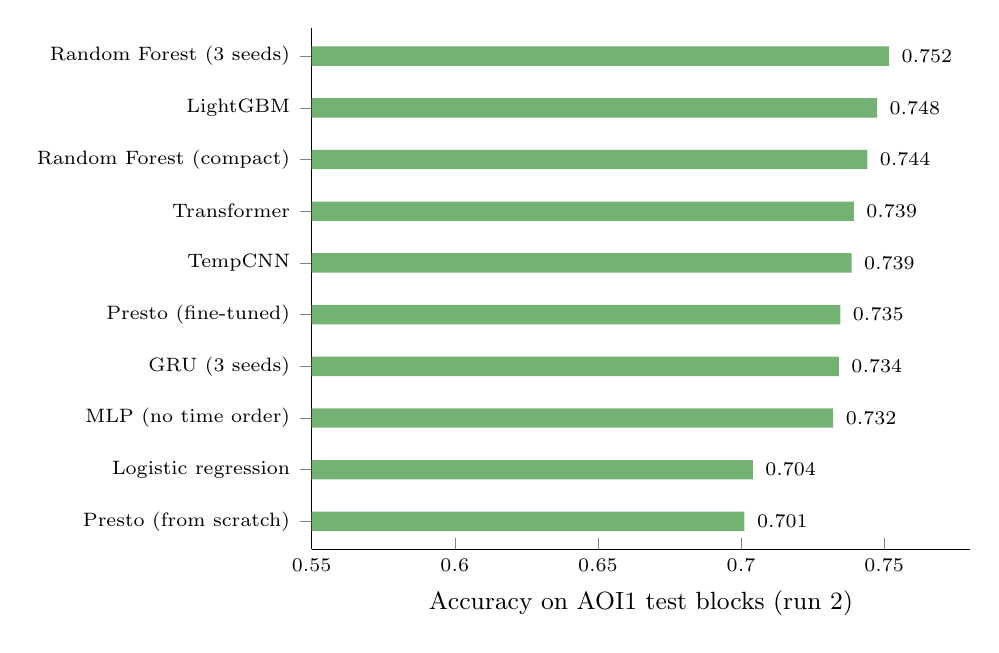
\begin{tikzpicture}
\begin{axis}[
  xbar, width=0.82\textwidth, height=8.2cm, xmin=0.55, xmax=0.78, bar width=7pt,
  ytick={0,...,9}, yticklabels={{Presto (from scratch)},{Logistic regression},{MLP (no time order)},{GRU (3 seeds)},{Presto (fine-tuned)},{TempCNN},{Transformer},{Random Forest (compact)},{LightGBM},{Random Forest (3 seeds)}},
  yticklabel style={font=\scriptsize}, xticklabel style={font=\scriptsize},
  xlabel={Accuracy on AOI1 test blocks (run 2)}, xlabel style={font=\small},
  nodes near coords, nodes near coords style={font=\scriptsize}, every node near coord/.append style={xshift=1pt},
  point meta=x, nodes near coords={\pgfmathprintnumber[fixed,precision=3]{\pgfplotspointmeta}},
  enlarge y limits=0.06, axis x line*=bottom, axis y line*=left]
\addplot[fill=green!45!black!55, draw=none] coordinates {
 (0.7012,0) (0.7041,1) (0.7322,2) (0.7342,3) (0.7347,4) (0.7386,5) (0.7394,6) (0.7441,7) (0.7475,8) (0.7517,9)};
\end{axis}
\end{tikzpicture}
\caption{Run 2: eleven models on the same AOI1 test blocks (axis starts at 0.55; majority class 0.199 not shown)}
\label{fig:models}
\end{figure}

Eight model families end within 2 points (73.2\% to 75.2\%); logistic regression is 4.8 points behind;
models that use time order (GRU, TempCNN~\cite{pelletier2019}, Transformer) do not clearly beat an MLP that ignores it.
Data and labels set the ceiling, not the algorithm, so the choice was made on cost
(Table~\ref{tab:cost}); LightGBM~\cite{ke2017} was proposed.

\begin{table}[htbp]
\centering\small
\caption{Accuracy against cost (run 2, AOI1; single-thread CPU)}
\label{tab:cost}
\begin{tabular}{L{4.2cm} r r r r}
\toprule
\textbf{Model} & \textbf{Accuracy} & \textbf{CPU ms / 1000 px} & \textbf{Size (MB)} & \textbf{RAM (MB)}\\
\midrule
Logistic regression & 0.704 & 0.016 & 1.2 & 321\\
MLP (no time order) & 0.732 & 3.8 & 0.29 & 550\\
Random Forest (compact) & 0.744 & 13.5 & 57.4 & 397\\
Random Forest (3 seeds) & 0.752 & 24.3 & 327.8 & 809\\
TempCNN & 0.739 & 31.9 & 0.6 & 570\\
\textbf{LightGBM (proposed)} & \textbf{0.748} & \textbf{35.8} & \textbf{1.98} & \textbf{549}\\
GRU (3 seeds) & 0.734 & 70.0 & 0.43 & 600\\
Transformer & 0.739 & 79.9 & 0.29 & 588\\
Presto (fine-tuned) & 0.735 & 2551 & 1.65 & 1200\\
\bottomrule
\end{tabular}
\end{table}

\subsection{Run 3: improvement ladder}
An improvement was kept only if validation macro-F1 rose by at least 0.002.
\begin{table}[htbp]
\centering\small
\caption{Improvement ladder (inputs per month; AOI1 validation change; AOI2 scores)}
\label{tab:ladder}
\begin{tabular}{L{4.1cm} c L{2.0cm} c c c}
\toprule
\textbf{Step} & \textbf{Inputs} & \textbf{AOI1 val.} & \textbf{AOI2 val.} & \textbf{AOI2 test} & \textbf{Decision}\\
 & \textbf{/ month} & \textbf{change} & \textbf{macro-F1} & \textbf{accuracy} & \\
\midrule
0 Benchmark (raw inputs) & 11 & start & 0.731 & 0.903 & start\\
1 + 4 indices, month flag & 16 & +0.0017 & 0.695 & 0.889 & dropped\\
2 + cleaned training labels & 11 & $-$0.030 & 0.681 & 0.909 & dropped\\
3 + neighbourhood inputs & 19 & +0.0024 & 0.742 & 0.912 & kept\\
\bottomrule
\end{tabular}
\end{table}
Neighbourhood inputs are the mean of NDVI, B8 and B11 over 3$\times$3 and 7$\times$7 windows and the spread
of NDVI; the 7$\times$7 window reaches 3 pixels, equal to the buffer, so no training pixel overlaps a
test block. Cleaning labels (removing edge pixels from training) hurt, because 29--47\% of test pixels
are edge pixels. The 3$\times$3 neighbour vote averages predicted probabilities of nearby test pixels;
window 3 was best on validation in both areas.

\subsection{Run 3 results in both areas}
\begin{table}[htbp]
\centering\small
\caption{Final results on both areas (all test pixels)}
\label{tab:both}
\begin{tabular}{L{6.2cm} c c}
\toprule
 & \textbf{AOI1 (E. Washington)} & \textbf{AOI2 (NE North Dakota)}\\
\midrule
Classes / test pixels & 14 / 99,238 & 9 / 144,922\\
Benchmark: accuracy / macro-F1 & 0.741 / 0.661 & 0.903 / 0.759\\
Improved inputs & 0.756 / 0.685 & 0.912 / 0.780\\
Improved + neighbour vote & \textbf{0.761 / 0.686} & \textbf{0.922 / 0.803}\\
Gain over benchmark (points) & +2.0 / +2.5 & +1.8 / +4.4\\
Test pixels on field edges & 47.0\% & 29.4\%\\
Accuracy on interior / edge pixels & 0.952 / 0.546 & 0.988 / 0.762\\
Share of errors on edge pixels & 89\% & 89\%\\
Final model (chosen on validation) & Average of 3 models & LightGBM\\
\bottomrule
\end{tabular}
\end{table}

\begin{figure}[htbp]
\centering
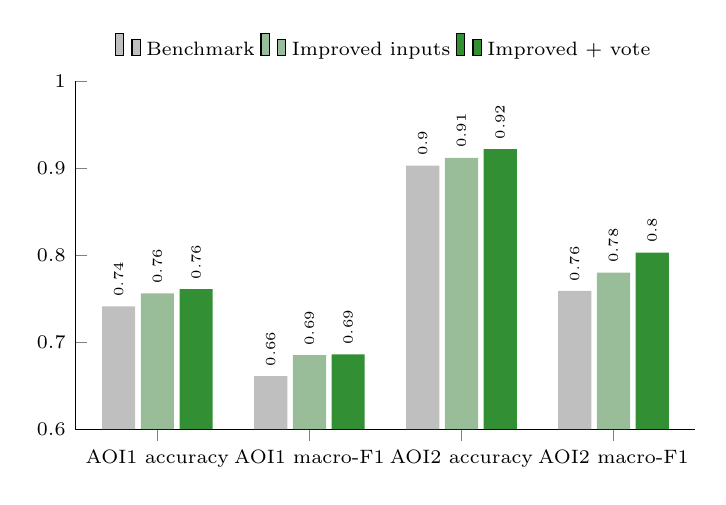
\begin{tikzpicture}
\begin{axis}[
  ybar, width=0.78\textwidth, height=6.0cm, ymin=0.6, ymax=1.0, bar width=12pt,
  symbolic x coords={AOI1 accuracy,AOI1 macro-F1,AOI2 accuracy,AOI2 macro-F1}, xtick=data,
  xticklabel style={font=\scriptsize}, yticklabel style={font=\scriptsize},
  legend style={font=\scriptsize, at={(0.5,1.03)}, anchor=south, legend columns=3, draw=none},
  nodes near coords, nodes near coords style={font=\tiny, rotate=90, anchor=west},
  enlarge x limits=0.18, axis x line*=bottom, axis y line*=left]
\addplot[fill=black!25, draw=none] coordinates {(AOI1 accuracy,0.741) (AOI1 macro-F1,0.661) (AOI2 accuracy,0.903) (AOI2 macro-F1,0.759)};
\addplot[fill=green!35!black!40, draw=none] coordinates {(AOI1 accuracy,0.756) (AOI1 macro-F1,0.685) (AOI2 accuracy,0.912) (AOI2 macro-F1,0.780)};
\addplot[fill=green!45!black!80, draw=none] coordinates {(AOI1 accuracy,0.761) (AOI1 macro-F1,0.686) (AOI2 accuracy,0.922) (AOI2 macro-F1,0.803)};
\legend{Benchmark, Improved inputs, Improved + vote}
\end{axis}
\end{tikzpicture}
\caption{Benchmark, improved inputs and neighbour vote in both areas (axis starts at 0.6)}
\label{fig:both}
\end{figure}

\textbf{How to quote the result.} AOI1: 76.1\% on all test pixels (95\% interval 72.1\% to 79.6\% over
test blocks), macro-F1 0.686; on field interiors 95.2\%. The improved pipeline is +2.0 points over the
benchmark (interval +1.0 to +3.0). Run-to-run noise is about 0.7 points, so differences under about
1 point are not reliable.

\textbf{Error analysis.} About 89\% of errors in both areas sit on pixels that touch another label;
67\% of AOI1 edge errors predict the neighbouring class (boundary bleed). Confusions are between
agronomically close classes: Alfalfa and Other Hay, Corn and Sweet Corn (AOI1); Spring Wheat and
Barley, Spring Wheat and Fallow/Idle (AOI2). Weakest AOI1 classes by F1 are Fallow/Idle (0.29) and
Other (0.29); strongest are Onions (0.91), Potatoes (0.86) and Alfalfa (0.85)
(Appendix~\ref{app:tests}, Table~\ref{tab:perclass}).

\subsection{Comparison with published work}\label{sec:papers}
\begin{table}[htbp]
\centering\small
\caption{GeoCrop crop-type results next to published studies (context, not a ranking)}
\label{tab:papers}
\begin{tabularx}{\textwidth}{L{2.8cm} L{1.6cm} L{3.3cm} Y L{1.9cm}}
\toprule
\textbf{Study} & \textbf{Unit} & \textbf{Labels / split} & \textbf{Result} & \textbf{Classes}\\
\midrule
GeoCrop (ours) & Pixel, 30~m & CDL 2022, all pixels; spatial blocks & AOI2 92.2\%; AOI1 76.1\% (interior 95.2\%) & 9 and 14\\
Tran et al.\ 2022~\cite{tran2022} & Pixel, 10~m & Good-quality CDL; 80/20 samples & 94\% South Dakota; 83\% California & 10 and 20\\
Li et al.\ 2024~\cite{li2024} & Pixel & Trusted CDL pixels & Corn/soybean F1 0.85--0.97 & --\\
PSE-TAE 2020~\cite{garnot2020} & Parcel & Parcel declarations & OA 94.2\%; RF 91.6\% & 20\\
BreizhCrops 2020~\cite{russwurm2020} & Parcel & Held-out region & Transformer 0.81, TempCNN 0.80, RF 0.78 & 9\\
Presto 2023~\cite{tseng2023} & Pixel series & Pre-trained & S2-Agri100 OA 68.9\% & --\\
Prithvi-EO-2.0 2024~\cite{szwarcman2024} & Chip & CDL, 3 dates & mIoU 48.6--50.7 & 13\\
\bottomrule
\end{tabularx}
\end{table}
AOI2 (92.2\%) is close to the 94\% reported for South Dakota, a similar northern-plains crop mix,
while using a stricter spatial split and no label-quality filter. AOI1 (76.1\%) is below the 83\% for
California but is a harder area with 47\% edge pixels. Parcel-level studies classify whole fields,
which removes the edge problem, so their numbers are not directly comparable. As in the papers, the
algorithm moves results by a few points, while labels and the evaluation unit move them by tens of
points. A like-for-like comparison needs the CDL confidence filter and matching class sets
(Iteration~2).

\textbf{Baseline model in the platform.} The platform currently runs the proposal-stage two-stage
Random Forest (single composite, seven features), retrained and saved for live inference. Its
held-out scores of 93\% (cropland) and 56\% (crop type) come from a random pixel split and are shown
in the portal with that caveat; under the spatial protocol a single-date input reaches only 26.7\%.
Replacing it with the selected pipeline is the first task of Iteration~2.

\section{Tools, Frameworks and Technologies}
\begin{table}[htbp]
\centering\small
\caption{Tools, frameworks and technologies}
\label{tab:tools}
\begin{tabularx}{\textwidth}{L{3.2cm} Y}
\toprule
\textbf{Area} & \textbf{Tools}\\
\midrule
Frontend & React 19, Vite, TypeScript, MapLibre GL JS, react-map-gl, pmtiles, TanStack Query, Zustand, React Router\\
Backend & Python 3.12, FastAPI, Pydantic, SQLAlchemy 2, GeoAlchemy2, Alembic, PyJWT, bcrypt, boto3\\
Geospatial & GDAL/rasterio, rio-tiler, TiTiler, shapely, pyproj, mercantile, mapbox-vector-tile, PostGIS 3.4\\
Processing & Celery, Redis 7\\
Storage & MinIO (S3 API), PostgreSQL 16\\
Machine learning & scikit-learn, LightGBM, PyTorch (deep models in the comparison), Presto, joblib, NumPy\\
Data & Google Earth Engine (Sentinel-2 export), USDA CDL, USDA NASS QuickStats\\
DevOps & Docker, Docker Compose, Nginx, Git\\
Testing & pytest, curl-based API checks, headless browser checks, custom tile benchmark\\
\bottomrule
\end{tabularx}
\end{table}

\section{Demonstration Evidence}\label{sec:demo}
\textbf{Rendering benchmark.} Table~\ref{tab:benchmark} compares the prototype's approach with the new
tile path on the same AOI1 crop-type result, measured through Nginx on a laptop.

\begin{table}[htbp]
\centering\small
\caption{Rendering benchmark on AOI1 (crop-type layer, zoom 12)}
\label{tab:benchmark}
\begin{tabularx}{\textwidth}{L{4.6cm} Y Y}
\toprule
\textbf{Measure} & \textbf{Prototype (GeoJSON)} & \textbf{GeoCrop (COG tiles)}\\
\midrule
Data for one screen of AOI1 & 43.3~MB (whole file) & 337~KB (24 tiles)\\
Objects the browser draws & 101,435 polygons ($\approx$750k vertices) & 24 PNG images\\
Server / parse time & 1,021~ms to parse the JSON only & cold tile median 47~ms, p95 54~ms\\
Cached tile latency & no caching & median 1~ms (Nginx hit)\\
Typical tile size & n/a & median 2.9~KB, max 44~KB\\
Storage of the same result & 43.3~MB GeoJSON & 222~KB compressed GeoTIFF\\
\bottomrule
\end{tabularx}
\end{table}

\begin{figure}[htbp]
\centering
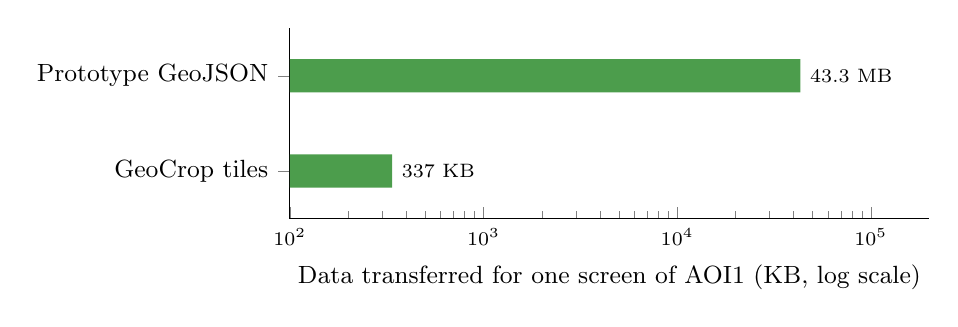
\begin{tikzpicture}
\begin{axis}[xbar, xmode=log, width=0.8\textwidth, height=4.0cm, bar width=12pt,
  symbolic y coords={GeoCrop tiles,Prototype GeoJSON}, ytick=data,
  xlabel={Data transferred for one screen of AOI1 (KB, log scale)}, xlabel style={font=\small},
  yticklabel style={font=\small}, xticklabel style={font=\scriptsize}, xmin=100, xmax=200000,
  enlarge y limits=0.5, axis x line*=bottom, axis y line*=left]
\addplot[fill=green!45!black!70, draw=none] coordinates {(337,GeoCrop tiles) (43300,Prototype GeoJSON)};
\node[anchor=west, font=\scriptsize] at (axis cs:337,GeoCrop tiles) {337 KB};
\node[anchor=west, font=\scriptsize] at (axis cs:43300,Prototype GeoJSON) {43.3 MB};
\end{axis}
\end{tikzpicture}
\caption{Data per screen: prototype against tile-based delivery (about 130 times less)}
\label{fig:benchmark}
\end{figure}

\textbf{Pipeline run.} Uploading the AOI1 Sentinel-2 GeoTIFF through a signed URL, ingesting it,
running the cropland and crop-type models block by block and publishing both layers took 57~s,
with each step visible on the Processing page. Loading the AOI1 demonstration data took about 5~s.

\textbf{Screenshots.} Figures~\ref{fig:shot-home}--\ref{fig:shot-status} show the running portal.

\begin{figure}[htbp]
\centering
\fbox{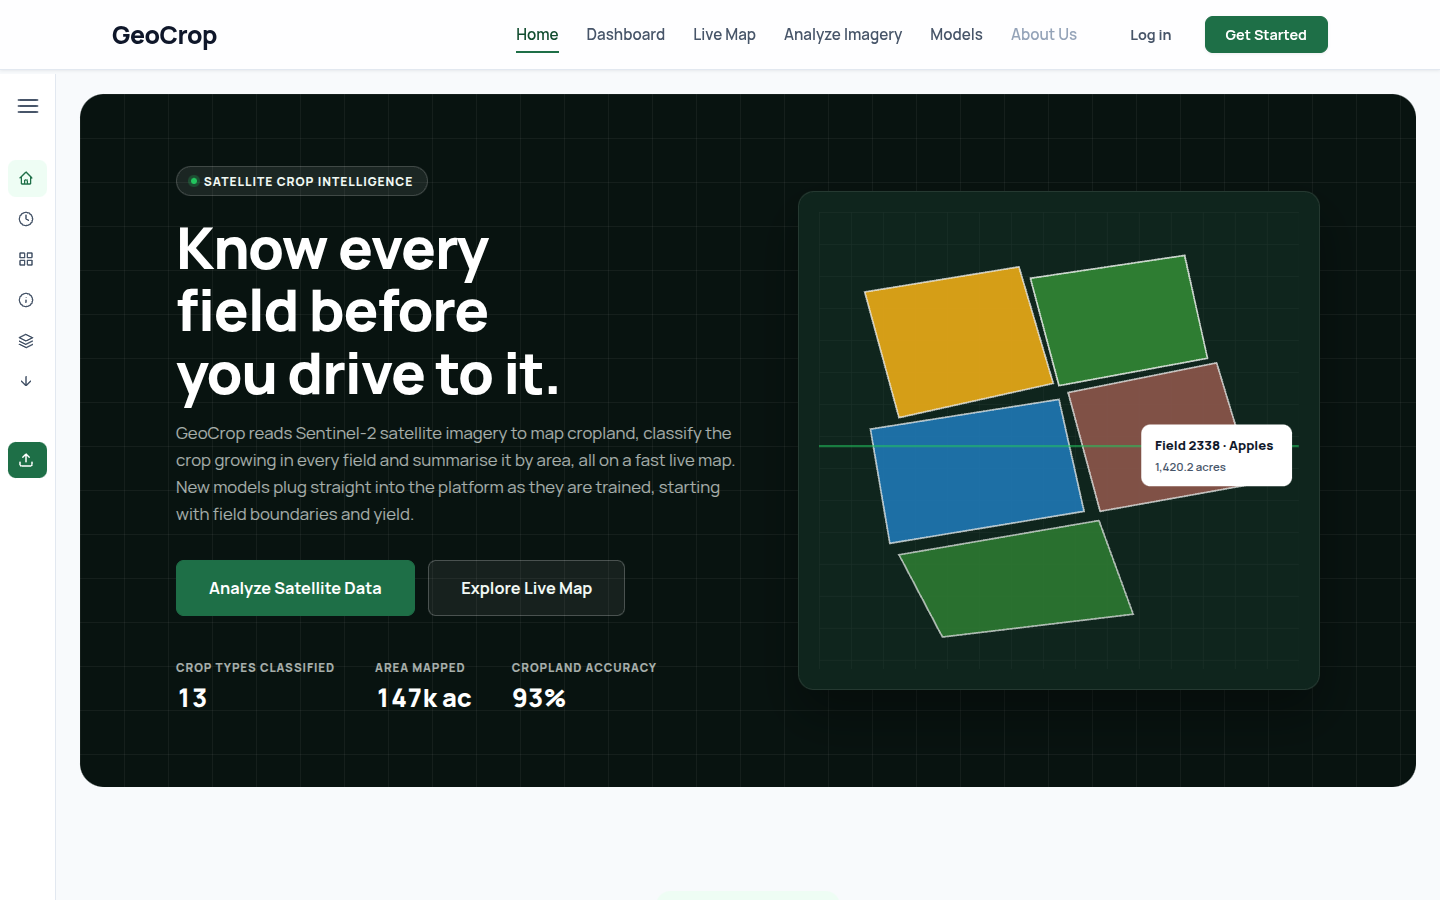
\includegraphics[width=0.92\textwidth]{figures/shot_home.png}}
\caption{Home page with live figures from the AOI1 results}
\label{fig:shot-home}
\end{figure}

\begin{figure}[htbp]
\centering
\fbox{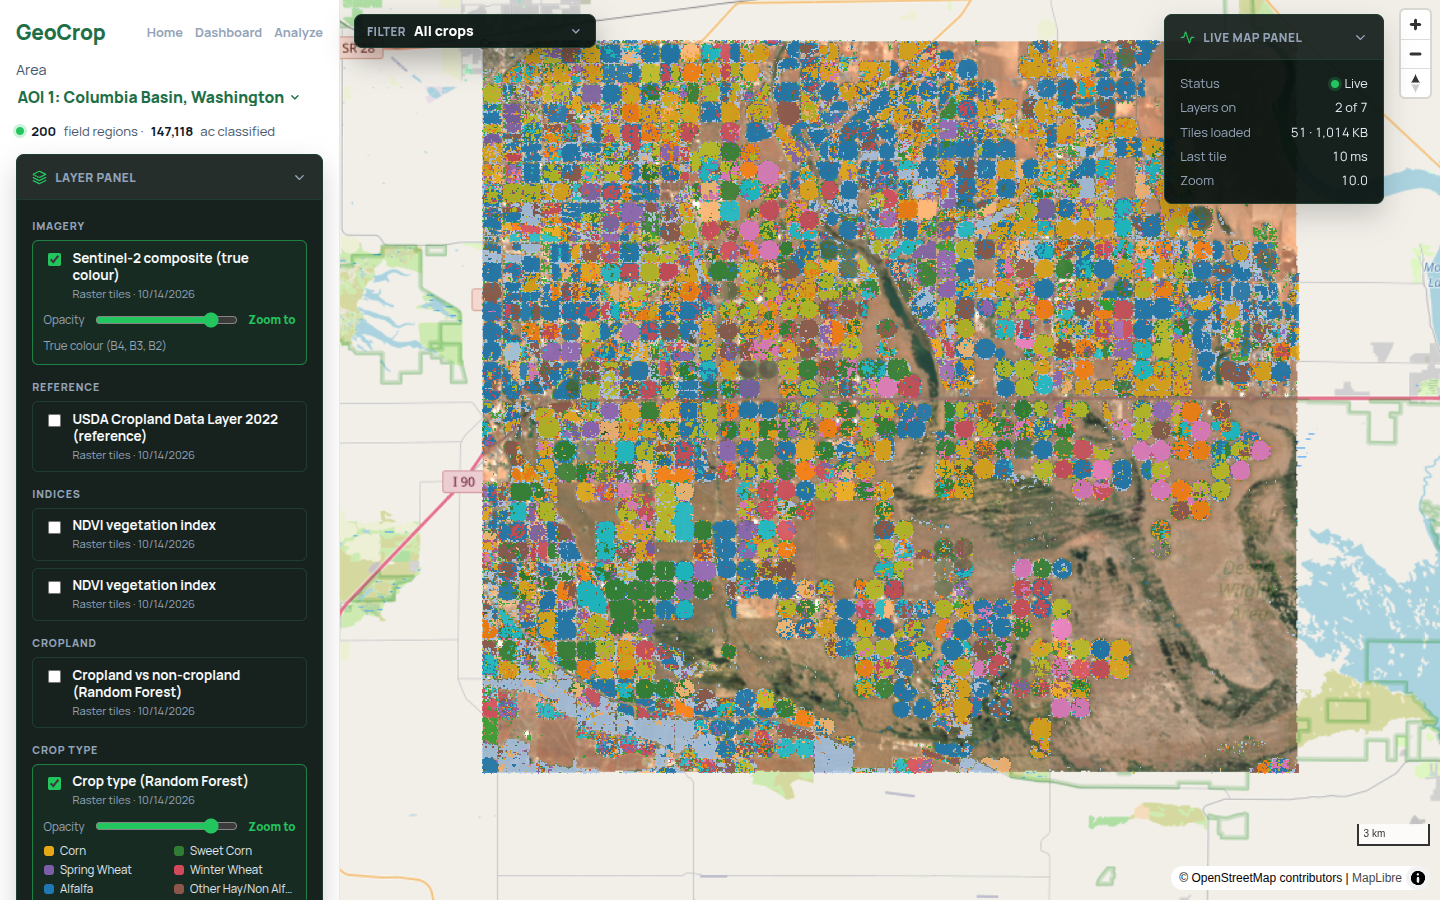
\includegraphics[width=0.92\textwidth]{figures/shot_map.png}}
\caption{Live Map workspace: layer panel, crop-type layer over Sentinel-2 imagery, crop filter and Live map panel (tiles loaded and latency)}
\label{fig:shot-map}
\end{figure}

\begin{figure}[htbp]
\centering
\fbox{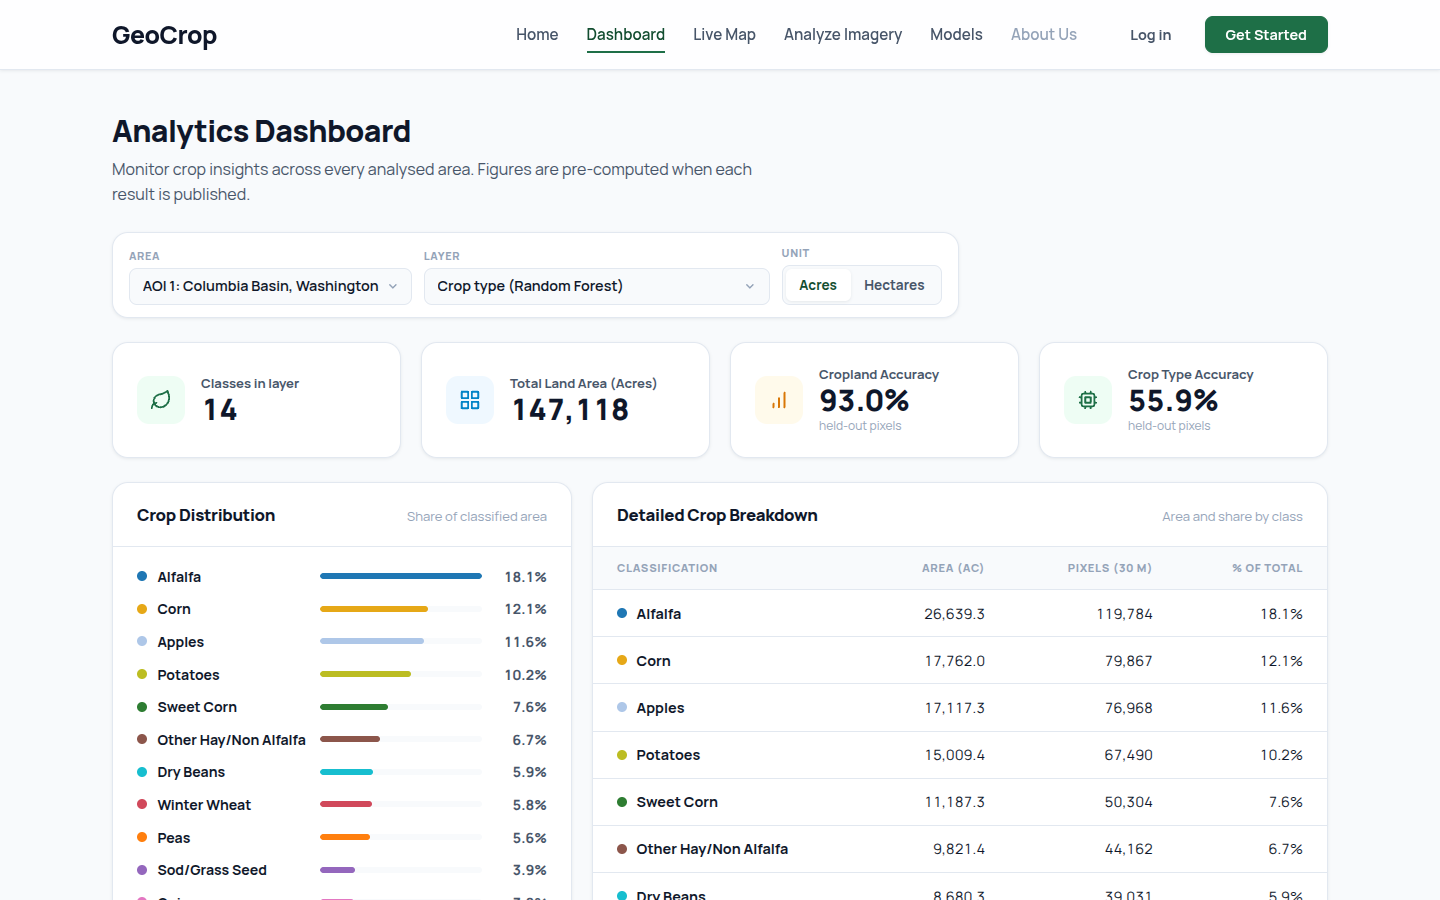
\includegraphics[width=0.92\textwidth]{figures/shot_dashboard.png}}
\caption{Analytics Dashboard: statistics from PostGIS and measured model accuracy}
\label{fig:shot-dashboard}
\end{figure}

\begin{figure}[htbp]
\centering
\fbox{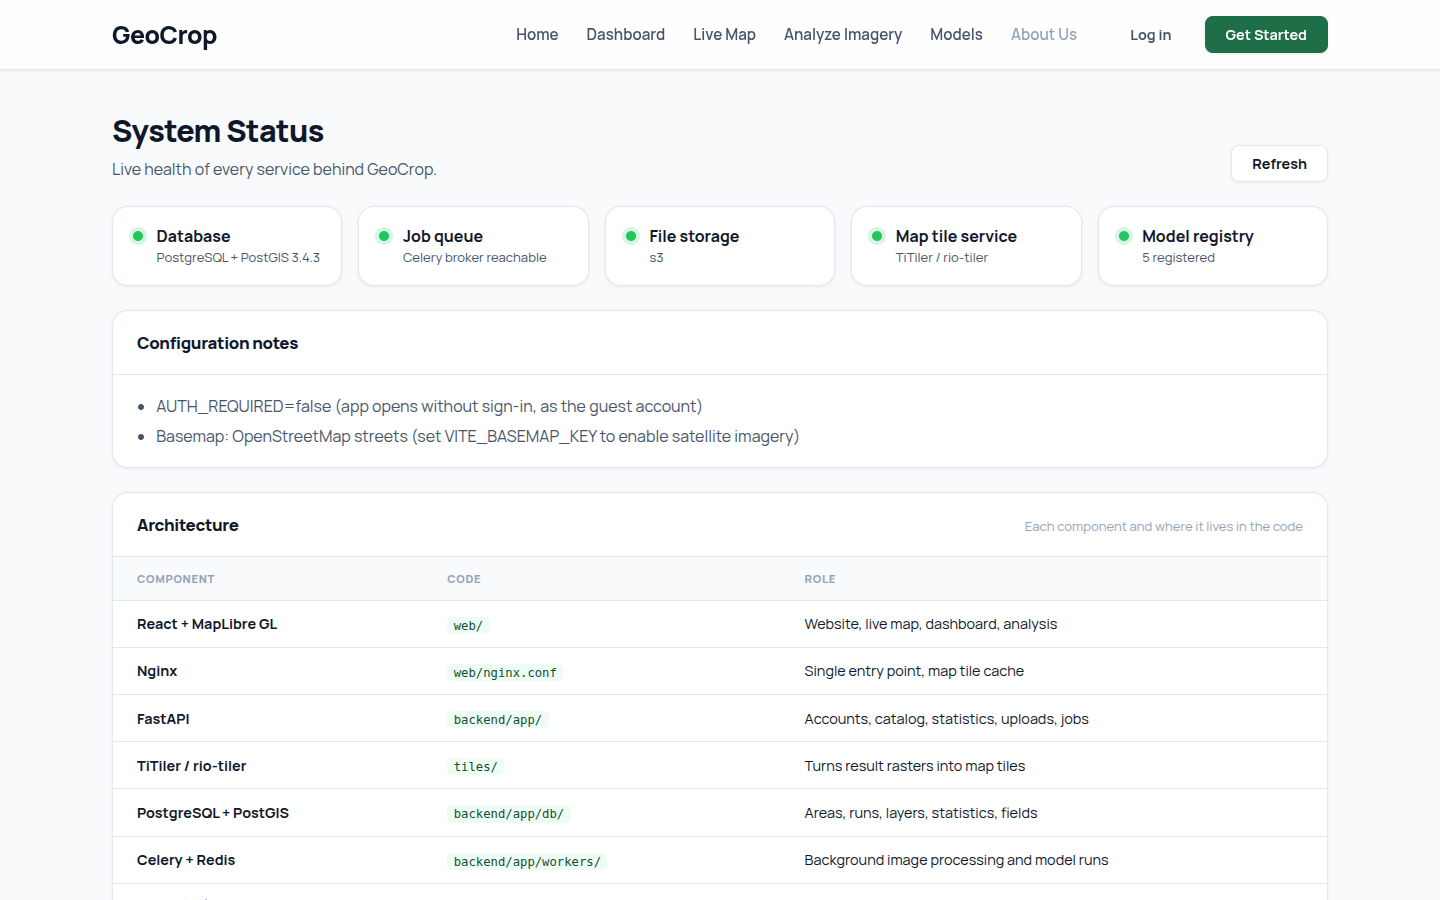
\includegraphics[width=0.92\textwidth]{figures/shot_status.png}}
\caption{System Status: health of every service and the architecture map}
\label{fig:shot-status}
\end{figure}

\subsection{Workflow feasibility and resource requirements}\label{sec:feasibility}
The panel found that the complexity and resource requirements of the complete workflow had not been
analysed, and that running it as one single flow may not be practical (P4, P5). Each stage was
therefore measured on its own on the AOI1 image (1,332$\times$1,239 pixels at 30~m, about
148,500~ha, 7 inputs per pixel). Every stage ran in a fresh process in the worker container, on an
8-core laptop CPU with 15~GB RAM, reading the image in 512$\times$512 blocks
(Table~\ref{tab:resources}).

\begin{table}[htbp]
\centering\small
\caption{Measured resource requirements of the complete workflow (AOI1, one fresh process per stage)}
\label{tab:resources}
\begin{tabularx}{\textwidth}{L{3.6cm} r r Y}
\toprule
\textbf{Stage} & \textbf{Time} & \textbf{Peak RAM} & \textbf{Storage / notes}\\
\midrule
Upload and validation & -- & -- & Input GeoTIFF 24.8~MB, sent directly to object storage\\
Cloud-optimised GeoTIFF & 0.7~s & 357~MB & 29.5~MB COG with overviews\\
Cropland model (RF) & 1.1~s load + 2.7~s & 395~MB & Model 71.6~MB; 1.11~M pixels classified\\
Crop-type model (baseline RF) & 2.5~s load + 7.5~s & \textbf{3,145~MB} & Model \textbf{1.57~GB}; 0.69~M cropland pixels\\
Crop-type model (LightGBM, proposed) & 35.8~ms / 1000~px & 549~MB & Model 1.98~MB (Table~\ref{tab:cost})\\
Publish results & -- & -- & Crop type 222~KB, cropland 63~KB compressed rasters; statistics in PostGIS\\
Full upload-to-map run & 57~s & -- & Includes transfer, queueing, storage writes and publishing\\
Idle platform (7 services) & -- & about 1.0~GB & Database 23~MB with AOI1 loaded\\
\bottomrule
\end{tabularx}
\end{table}

Three findings follow. First, the compute itself is small: all model and conversion stages together
take about 15~s; the rest of the 57~s run is transfer, queueing and publishing. Second, memory, not
time, is the real limit. The baseline Random Forest crop-type model needs 1.57~GB on disk and about
3.1~GB of RAM, so two parallel runs would already need more than 6~GB. The proposed LightGBM model
needs 549~MB (measured by the model track, Table~\ref{tab:cost}) at about the same accuracy, which makes the full workflow fit on a normal laptop.
Third, results are small once stored as compressed rasters (285~KB for both layers against 43.3~MB
of GeoJSON), so storage grows slowly as AOIs and models are added.

The design therefore avoids a single flow. Ingest, each model and publishing are separate queued
steps that run in background workers, one model at a time in dependency order, with progress and
errors recorded per step. A failed or heavy step does not block the map, the API or other jobs, and
workers can be added on another machine without changing the code. Users never load the whole
dataset: the map requests only the tiles in view.

\section{Iteration Outcome}
Iteration 1 met its objectives. The architecture track delivered a working platform that reduces the
data for one screen from 43.3~MB to 337~KB, serves cold tiles in 47~ms and cached tiles in 1~ms,
analyses uploaded imagery end to end in under a minute, and accepts new models by folder and
manifest. The model track established a fair evaluation protocol, showed that a time series is the
key input and that model family matters little, selected a small CPU-only LightGBM pipeline
(76.1\% AOI1, 92.2\% AOI2) and located the remaining errors on field edges. Measuring every workflow stage answered the panel's feasibility question: compute is small,
memory is the limit, and the selected LightGBM model removes the 3.1~GB bottleneck of the baseline.
The main open items are
integrating the selected pipeline into the platform, the CDL confidence rule, the cross-area test,
and the boundary and yield models.

\chapter{Testing and Early Validation}

\section{Testing Strategy}
Testing follows the two tracks. The platform is tested from the smallest unit (the model registry)
up to the whole system in a browser, with a dedicated performance benchmark because performance is
the main design goal. The models are validated by an evaluation protocol designed to avoid
optimistic results: spatial block split, validation-only decisions, a single test pass, intervals
and per-class scores. Every defect found was fixed and re-tested, and the fix is recorded in the
repository history.

\textbf{Revised evaluation criteria.} The panel found that the proposal's evaluation criteria did not
measure the project's real challenges and named usability, performance and integration as the main
concerns, together with a lightweight system (P2, P3). The criteria were therefore rewritten so that
each concern has a metric, a target and a measured value (Table~\ref{tab:evalcriteria}). Model
accuracy remains a criterion, but is no longer the only one.

\begin{table}[htbp]
\centering\small
\caption{Revised evaluation criteria and status at mid-term}
\label{tab:evalcriteria}
\begin{tabularx}{\textwidth}{L{1.9cm} Y L{2.2cm} L{2.9cm}}
\toprule
\textbf{Concern} & \textbf{Metric} & \textbf{Target} & \textbf{Measured (status)}\\
\midrule
\multirow{4}{*}{Performance} & Map data for one screen & $<$1~MB & 337~KB (met)\\
 & Cold / cached tile latency (median) & $<$300 / $<$50~ms & 47 / 1~ms (met)\\
 & Upload to map for an AOI-sized image & $<$2~min & 57~s (met)\\
 & Layers usable at once without lag & $\geq$8 & Not measured yet\\
\midrule
\multirow{3}{*}{Lightweight} & Peak RAM per workflow stage & Fits a laptop & 0.36--3.1~GB, fits 15~GB (met; Table~\ref{tab:resources})\\
 & Selected crop-type model: size, CPU cost & CPU only, tens of MB & 1.98~MB, 35.8~ms/1000~px (met)\\
 & Whole platform on one host & One command & 7 services, 1.0~GB idle (met)\\
\midrule
\multirow{3}{*}{Integration} & Upload reaches the map without manual steps & All steps automatic & TC-11 (met)\\
 & New model added by folder and manifest only & No other change & TC-03 (met)\\
 & Layers from different models and images on one map & Same catalogue & 6 layers on AOI1 (met)\\
\midrule
\multirow{2}{*}{Usability} & Legends, readable errors, phone and desktop widths & NFR-U1--U3 & Checked (met)\\
 & Task success and questionnaire score (SUS) in a user study & $\geq$90\%, SUS $\geq$68 & Planned, Iteration 2\\
\midrule
Model quality & Accuracy and macro-F1 on spatial test blocks, with 95\% intervals & Reported honestly & AOI1 76.1\% / 0.686; AOI2 92.2\% / 0.803\\
\bottomrule
\end{tabularx}
\end{table}

\section{Test Levels and Techniques}
\begin{table}[htbp]
\centering\small
\caption{Test levels and techniques}
\label{tab:levels}
\begin{tabularx}{\textwidth}{L{2.8cm} Y L{3.0cm}}
\toprule
\textbf{Level} & \textbf{What and how} & \textbf{Tooling}\\
\midrule
Unit & Registry discovery, dependency planning, error messages, placeholder behaviour, add-a-model flow, on small synthetic rasters. & pytest\\
Integration & Every API route through Nginx with real data in PostGIS and MinIO; tile responses and cache headers; PMTiles range reads with CORS. & curl, scripted checks\\
System / end-to-end & Upload to map; re-analysis; Live Map filter, field search and inspection; dashboard; cold start of the stack. & Headless and interactive browser\\
Performance & Data per screen, cold and cached tile latency, tile sizes, parse cost of the old approach. & \code{tools/benchmark_tiles.py}\\
Model validation & Spatial block test, bootstrap intervals, per-class scores, cost per 1000 pixels. & Evaluation notebooks\\
\bottomrule
\end{tabularx}
\end{table}

\section{Test Cases}
\begin{table}[htbp]
\centering\small
\caption{Test cases (details in Appendix~\ref{app:tests})}
\label{tab:testcases}
\begin{tabularx}{\textwidth}{L{1.1cm} Y L{2.0cm}}
\toprule
\textbf{ID} & \textbf{Test} & \textbf{Requirement}\\
\midrule
TC-01 & Built-in models load without errors & FR-REG-01\\
TC-02 & Dependencies resolve in order (crop type after cropland; yield after both) & FR-REG-03\\
TC-03 & Add a model by copying the template and editing only the manifest & FR-REG-01, UC-11\\
TC-04 & Placeholder model produces no data & FR-REG-04\\
TC-05 & Raster tiles return PNG with immutable cache headers & FR-VIS-03\\
TC-06 & Outside-raster tile returns 204; cached tile served by Nginx & FR-VIS-03, NFR-P2\\
TC-07 & Statistics return area per class for the crop-type layer & FR-CAT-02\\
TC-08 & Point query returns crop and cropland labels & FR-VIS-04\\
TC-09 & Crop filter shows only the selected crop & FR-VIS-05\\
TC-10 & PMTiles range read (206) with CORS & FR-CAT-03\\
TC-11 & Upload Sentinel-2 image and run cropland + crop type & FR-ING-01..05\\
TC-12 & Re-run NDVI model on an existing image & FR-ING-07\\
TC-13 & Upload a 1-band file & FR-ING-03\\
TC-14 & Rendering benchmark & NFR-P1, NFR-P2\\
TC-15 & Cold start of the full stack & NFR-R1\\
\bottomrule
\end{tabularx}
\end{table}

\section{Test Results}
\begin{table}[htbp]
\centering\small
\caption{Test results}
\label{tab:testresults}
\begin{tabularx}{\textwidth}{L{1.1cm} Y L{1.3cm}}
\toprule
\textbf{ID} & \textbf{Observed result} & \textbf{Status}\\
\midrule
TC-01--04 & 5 of 5 pytest cases passed in 0.4~s. & Pass\\
TC-05 & Four raster layers returned 256$\times$256 PNG tiles with \code{public, max-age=31536000, immutable}. & Pass\\
TC-06 & Out-of-range tiles returned 204; repeated requests showed \code{X-Cache-Status: HIT}. & Pass\\
TC-07 & Crop-type layer: 14 classes, 59,537~ha (147,118 acres) classified; Alfalfa 18.1\%, Corn 12.1\%, Apples 11.6\%. & Pass\\
TC-08 & Clicking a pivot field returned ``Alfalfa'' and ``Cropland'' (API) and ``Spring Wheat'' in another field (browser). & Pass\\
TC-09 & Filter ``Apples'' left only apple pixels over the imagery. & Pass\\
TC-10 & PMTiles range request returned 206 with \code{Access-Control-Allow-Origin}. & Pass\\
TC-11 & Job completed in 57~s; all six steps done; both layers listed on the map. & Pass\\
TC-12 & NDVI run completed in about 1~s; new layer listed. & Pass\\
TC-13 & Job failed with ``The image has 1 bands. Expected a Sentinel-2 stack (B2, B3, B4, B8, B11, B12 and optionally NDVI).'' & Pass\\
TC-14 & 337~KB per screen, cold 47~ms median, cached 1~ms (Table~\ref{tab:benchmark}). & Pass\\
TC-15 & After \code{down} and \code{up -d}, all seven services healthy; health status ``ok''. & Pass\\
\bottomrule
\end{tabularx}
\end{table}

\section{Acceptance Testing / Validation}
The acceptance checks of Table~\ref{tab:acceptance} were run on the integrated system: all platform
checks passed. Crop-type validation followed the protocol of Section~\ref{sec:protocol} and is
summarised in Table~\ref{tab:both}; live inference in the platform was also compared with the
training-time raster for AOI1, and class areas agreed closely (Apples 6,927~ha in both; Alfalfa
11,340~ha against 10,781~ha, the difference coming from masking by the predicted rather than the
reference cropland). A supervised acceptance session with the supervisor and external co-supervisor
is planned at the mid-term demonstration.

\section{Edge and Failure Cases}
\begin{itemize}
  \item Non-GeoTIFF files are rejected before upload; images without a CRS or with an unsupported band
        count fail the job with a readable reason (TC-13).
  \item Placeholder models are skipped and marked ``not available'' instead of failing the job.
  \item Requests for tiles outside a raster return 204, which the map treats as empty.
  \item Points outside the data return ``No data''.
  \item A broken model manifest is reported on the Models and Status pages while other models load.
  \item Float imagery with NaN no-data values is handled (stored as null in the catalogue).
\end{itemize}

\section{Defects and Corrective Actions}
\begin{table}[htbp]
\centering\small
\caption{Defects found during Iteration 1 and corrective actions}
\label{tab:defects}
\begin{tabularx}{\textwidth}{L{0.6cm} Y Y}
\toprule
\textbf{No.} & \textbf{Defect} & \textbf{Corrective action}\\
\midrule
1 & Official MinIO images no longer available from public registries. & Pinned Bitnami build of the same MinIO server; documented.\\
2 & Table name \code{layer} clashed with the PostGIS \code{topology.layer} table. & Renamed to \code{map_layer}; migrations limited to GeoCrop tables.\\
3 & rasterio failed in slim containers (missing \code{libexpat}). & Added the system library to both images.\\
4 & MapLibre web worker failed to load (wrong path, then wrong MIME type for \code{.mjs}). & Explicit worker URL; Nginx MIME type rule.\\
5 & Bucket initialisation raced MinIO start-up on cold boot. & Retry loop in the initialiser; cold start re-tested.\\
6 & Uploaded-image layers returned 404 tiles: NaN no-data could not be serialised. & Store non-finite no-data as null; repaired existing rows.\\
7 & Browser kept an old page after a new build. & \code{no-cache} for the page shell, long cache for hashed assets.\\
8 & Site lost the API after a backend container was rebuilt (stale address). & Nginx resolves services through Docker DNS at request time.\\
\bottomrule
\end{tabularx}
\end{table}

\section{Current Validation Status}
\begin{itemize}
  \item \textbf{Platform:} all 15 test cases pass; performance targets NFR-P1, NFR-P2 and NFR-P4 are met
        on AOI1; NFR-P3 (eight or more layers visible at once) has not been measured yet.
  \item \textbf{Models:} crop-type pipeline validated on two areas with spatial blocks and intervals;
        not yet validated across areas or against field data; CDL confidence rule pending.
  \item \textbf{Not yet validated:} boundary accuracy (IoU, area error), yield metrics, multi-user
        load, and the integrated LightGBM pipeline's serving cost.
\end{itemize}

\chapter{Project Management and Development Evidence}

\section{Work Completed}
\begin{itemize}
  \item Literature review extended from 11 proposal papers to 15 summarised studies, with eight
        crop-type papers read for the model comparison.
  \item Proposal-stage prototype (Django, Leaflet, offline Random Forest scripts) analysed and its
        rendering bottleneck measured.
  \item New platform repository with seven containerised services, database migration, model
        registry, processing pipeline, tile service and Web GIS portal (Chapter~\ref{ch:iter1}).
  \item AOI1 data prepared as COG (imagery and CDL), baseline models retrained and saved for live
        inference, field-region PMTiles built, demonstration data loaded.
  \item Monthly 2022 Sentinel-2 composites for AOI1 and AOI2; spatial evaluation protocol; 11-model
        comparison with cost; improvement ladder; error analysis; comparison with papers.
  \item Rendering benchmark, 15 platform test cases, and project documentation (architecture,
        status, upgrade path, adding a model, running without Docker, demonstration script).
\end{itemize}

\section{Work Remaining}
\begin{itemize}
  \item Integrate the LightGBM crop-type pipeline (monthly composites, neighbourhood inputs, vote) as
        a registry model; monthly-composite ingestion.
  \item CDL confidence rule; AOI2 interval and interior table; cross-area test; exports for the
        remaining AOIs.
  \item Field-boundary model and boundary/area validation (IoU, area error, acreage against NASS).
  \item Yield data preparation and yield model ($R^2$, RMSE, MAE).
  \item Multi-image upload, mosaics and an all-areas map view.
  \item Hardening (signed tile access, required sign-in, monitoring), deployment and final evaluation.
\end{itemize}

\section{Individual Responsibilities}
\begin{table}[htbp]
\centering\small
\caption{Individual responsibilities}
\label{tab:resp}
\begin{tabularx}{\textwidth}{L{3.4cm} L{3.0cm} Y}
\toprule
\textbf{Member} & \textbf{Role} & \textbf{Responsibilities}\\
\midrule
Huzaifa Bin Khalid (22I-2332) & Architecture and platform & System architecture; performance analysis; data and storage design; tile delivery; processing pipeline; model registry; Web GIS portal; deployment configuration; benchmark and platform testing.\\
Saneed Ullah (23I-2568) & Crop-type model evaluation & Monthly composite preparation; evaluation protocol; model comparison and cost measurement; improvement experiments; error analysis; comparison with reference papers.\\
Taha Bashir Awan (23I-0824) & Crop-type model evaluation & Model experiments and comparison across families; evaluation and analysis of results; comparison with reference papers.\\
\bottomrule
\end{tabularx}
\end{table}

\section{Contribution of Each Team Member}
\textbf{Huzaifa Bin Khalid} defined the base architecture with performance as the main constraint,
identified and measured the prototype's rendering problem, chose and integrated the technologies
(COG, TiTiler, PMTiles, MapLibre, FastAPI, PostGIS, Celery, MinIO), designed the plug-in model
registry and processing pipeline, delivered the Web GIS portal styled after the original prototype,
and validated the system with the benchmark and end-to-end tests.

\textbf{Saneed Ullah and Taha Bashir Awan} carried out the crop-type model evaluation and comparison:
the two study areas and their monthly composites, the spatial block protocol, the eleven-model
comparison with speed, size and memory, the run-3 improvements (neighbourhood inputs and neighbour
vote), the per-class and edge-pixel error analysis, and the comparison with eight reference papers,
leading to the LightGBM recommendation. The crop-type results report was prepared by Saneed Ullah.

All members share integration, documentation and the final evaluation.

\section{Repository and Version Control Evidence}
\begin{itemize}
  \item \textbf{Prototype repository} (\code{zzzzzzzzzzzzz}, Git): Django prototype, offline training
        scripts and proposal-stage results; 11 commits from 1 to 8 September 2026.
  \item \textbf{Platform repository} (\code{geocrop-platform}, Git, branch \code{main}): the
        Iteration 1 architecture and implementation, data tools, extended training scripts, tests
        and documentation; six commits on 14 October 2026 (Appendix~\ref{app:repo}). Large data and
        model files are excluded from Git and reproduced with \code{make data}.
  \item \textbf{Research notebooks:} \code{GeoCrop_CropType_Model_Benchmark.ipynb} (runs 1 and 2,
        model families, cost, bootstrap) and \code{GeoCrop_Accuracy_Boost.ipynb} (run 3), with the
        crop-type results report dated 14 October 2026.
\end{itemize}

\section{Milestones and Commit Evidence}
\begin{table}[htbp]
\centering\small
\caption{Milestones}
\label{tab:milestones}
\begin{tabularx}{\textwidth}{L{2.6cm} Y L{3.6cm}}
\toprule
\textbf{Date (2026)} & \textbf{Milestone} & \textbf{Evidence}\\
\midrule
1--8 Sep & Prototype: Django portal, Live Map, Analysis Studio, two-stage Random Forest & Prototype commits \code{f10912e}--\code{3760eae}\\
7--8 Sep & Proposal document & Proposal \LaTeX{} source\\
11 Sep & Proposal defence & Proposal slides\\
Sep--Oct & Monthly composites; runs 1--3; paper comparison & Notebooks; results report (14 Oct)\\
14 Oct & Platform repository, services, registry, portal & Commits \code{f056a54}--\code{fae4751}\\
14 Oct & Reliability fixes; optional sign-in; UI after the prototype & Commits \code{efc3c68}--\code{4c631c9}\\
15 Oct & Mid-report & This document\\
\bottomrule
\end{tabularx}
\end{table}

\section{Tools and Tool-Assisted Development}\label{sec:tools-assisted}
Standard tools were used throughout: Git for version control, Docker for reproducible services,
Jupyter notebooks for experiments, Google Earth Engine for imagery export and \LaTeX{} for
documentation.

\textbf{AI-assisted development.} An AI coding assistant (Anthropic Claude, used through Claude Code)
was used on the architecture track to speed up implementation: generating parts of the platform code
and configuration from the team's architecture and requirements, diagnosing deployment problems, and
drafting documentation, including parts of this report. The architecture, technology choices,
requirements, acceptance criteria and evaluation targets were set by the team; all generated code was
run, tested and reviewed against the tests and benchmark reported here, and the team remains
responsible for it. This goes beyond the boundary stated in the proposal (generative AI limited to
documentation and presentation support) and is recorded as a deviation in
Section~3.8. The models, preprocessing and evaluation design of the research track are the team's
own work.

\section{External Components and Dependencies}\label{sec:external}
\begin{table}[htbp]
\centering\small
\caption{External components, data and licences}
\label{tab:external}
\begin{tabularx}{\textwidth}{L{3.6cm} Y L{3.0cm}}
\toprule
\textbf{Component} & \textbf{Use} & \textbf{Licence / terms}\\
\midrule
Sentinel-2 imagery & Model input & Copernicus open licence\\
USDA CDL, USDA NASS & Labels, yield statistics & U.S. public domain\\
OpenStreetMap tiles & Default basemap & ODbL, attribution shown\\
MapLibre GL JS, react-map-gl & Map rendering & BSD-3, MIT\\
React, Vite, TanStack Query, Zustand & Frontend & MIT\\
FastAPI, Pydantic, SQLAlchemy, Alembic & API & MIT\\
TiTiler, rio-tiler, rasterio, GDAL & Raster processing and tiles & MIT, BSD-3\\
PostgreSQL, PostGIS & Database & PostgreSQL licence, GPL-2\\
Celery, Redis & Jobs & BSD-3, BSD-3 (Redis 7)\\
MinIO (Bitnami build) & Object storage & AGPL-3\\
scikit-learn, LightGBM, PyTorch & Models & BSD-3, MIT, BSD-3\\
Presto (research comparison) & Pre-trained model & MIT\\
Nginx, Docker & Edge, containers & BSD-2, Apache-2\\
\bottomrule
\end{tabularx}
\end{table}

\section{Risks and Mitigation}
\begin{table}[htbp]
\centering\small
\caption{Risks and mitigation}
\label{tab:risks}
\begin{tabularx}{\textwidth}{L{3.6cm} L{1.4cm} Y}
\toprule
\textbf{Risk} & \textbf{Level} & \textbf{Mitigation}\\
\midrule
CDL label noise and mixed edge pixels & High & Report all-pixel scores first; add one fixed CDL confidence rule; neighbourhood inputs and vote; field-level classification later.\\
Poor generalisation to new areas or years & High & Cross-area test in Iteration 2; more AOIs; model cards state valid regions.\\
Cloudy or missing imagery & Medium & Monthly composites with linear gap filling; validation of inputs at ingest.\\
Limited yield ground truth & High & Use county-level NASS data and evaluate at that scale; state granularity clearly.\\
Model size and serving cost & Medium & Baseline crop-type model measured at 3.1~GB RAM; replace with LightGBM (549~MB); measure every stage again after integration.\\
Usability not yet tested with users & Medium & Task-based user study with questionnaire in Iteration 2; findings fed into the portal.\\
Integration of research pipeline & Medium & Common plug-in contract; integration first in Iteration 2.\\
Dependency or registry changes (e.g.\ MinIO images) & Low & Pinned image versions; S3-compatible abstraction allows swapping.\\
Team time and coordination & Medium & Two parallel tracks with a shared contract; iteration reviews.\\
\bottomrule
\end{tabularx}
\end{table}

\section{Security and Privacy Considerations}
\begin{itemize}
  \item Passwords are hashed with bcrypt; sessions use signed JWTs; sign-in can be made mandatory with
        one setting (currently optional so the portal opens directly, which is shown on the status
        page).
  \item Secrets are read from environment variables; the repository contains only an example file.
  \item Areas and layers are filtered by owner or public flag in every catalogue query.
  \item Upload URLs are signed, short-lived and limited to one object; only vector tiles are publicly
        readable in storage.
  \item The tile service applies styles from the database, not from request parameters; internal
        routes require a service token.
  \item Uploaded or partner-provided data is not published; result layers of uploads are private to
        the uploading account.
\end{itemize}

\section{Current Limitations}
\begin{itemize}
  \item The platform runs the proposal-stage baseline crop-type model; the selected LightGBM pipeline
        is not integrated yet.
  \item Accuracy is agreement with the CDL for one year and two areas; no cross-area or field-survey
        validation yet.
  \item Field regions are derived from crop-type output, not from a boundary model.
  \item Yield estimation is not implemented.
  \item Upload supports one stacked GeoTIFF at a time; \code{.SAFE} products, cloud masking and
        mosaics are not supported yet.
  \item Tile URLs are not individually authorised; the default basemap is OpenStreetMap streets until
        a provider key is configured.
  \item The system runs on a single host; load with many concurrent users has not been tested.
\end{itemize}

\chapter{Remaining FYP Plan}\label{ch:remaining}

\section{Remaining Scope}
The remaining scope completes the satellite-to-GIS chain on top of the platform built in Iteration 1:
the selected crop-type pipeline in production use, a dedicated field-boundary model with area
validation, yield estimation, wider evaluation across areas, and a hardened, deployed system.

\section{Remaining Modules and Features}
\begin{table}[htbp]
\centering\small
\caption{Remaining modules and features}
\label{tab:remaining}
\begin{tabularx}{\textwidth}{L{3.6cm} Y L{1.8cm}}
\toprule
\textbf{Module} & \textbf{Feature} & \textbf{Iteration}\\
\midrule
M1 Data preparation & Monthly-composite ingestion in the pipeline; exports for remaining AOIs; optional cloud mask & 2, 3\\
M2 Crop mapping & LightGBM crop-type pipeline as a registry model; CDL confidence rule; cross-area test; field-level classification & 2, 3\\
M3 Boundaries and area & Field-boundary model; polygon simplification; IoU and area error; acreage against NASS & 3\\
M4 Yield & NASS yield preparation; yield model; county and field summaries & 3, 4\\
M5 Processing pipeline & Multi-image upload; batch progress; mosaics & 2\\
M8 Web GIS portal & All-areas view; compare runs; yield layers and dashboard; exports (GeoJSON, CSV) & 2--4\\
Hardening & Required sign-in, signed tile access, monitoring, load test, provider basemap & 4\\
\bottomrule
\end{tabularx}
\end{table}

\section{Remaining Iterations}
\begin{itemize}
  \item \textbf{Iteration 2 (mid-Oct -- Dec 2026, FYP-1 end):} crop-type pipeline integration, CDL
        confidence rule, AOI2 interval, cross-area test, multi-image upload and all-areas view,
        serving-cost measurement.
  \item \textbf{Iteration 3 (Feb -- Mar 2027, FYP-2):} field-boundary model and area validation; yield
        data and first yield model; more AOIs; field-level crop classification experiment.
  \item \textbf{Iteration 4 (Apr -- May 2027, FYP-2):} yield layers and dashboard, end-to-end evaluation
        against the success criteria, hardening, deployment, final report and demonstration.
\end{itemize}

\section{Implementation Plan}
New models are added through the registry (task and manifest), so the API, schema and interface
remain stable. The LightGBM pipeline is packaged with its saved model, feature definition and
metrics file; the ingest step gains a monthly-composite path. The boundary model writes a raster
or polygons that the existing vector-tile builder publishes as PMTiles. The yield model reads the
crop-type layer and satellite features and writes a continuous raster plus county summaries. The
portal adds layer groups and dashboard panels driven by the catalogue.

\section{Testing and Validation Plan}
\begin{itemize}
  \item Unit tests for each new model task (validation, outputs, metrics) and the extended pipeline.
  \item Integration and end-to-end tests repeated for every release; benchmark re-run with the new
        model and with several areas and layers visible.
  \item Crop type: all-pixel and CDL-confidence scores, cross-area test, per-class scores, intervals.
  \item Boundaries: IoU/Dice against reference boundaries and area error; acreage against USDA NASS.
  \item Yield: $R^2$, RMSE and MAE on held-out years or counties.
  \item Usability study (P3): five to eight participants, including the supervisors and, if
        possible, an agricultural user, complete set tasks (find a crop, compare two layers, upload
        an image); task success, time and a System Usability Scale questionnaire are recorded.
  \item Resource measurement repeated for every new model (time, peak RAM, storage), as in
        Table~\ref{tab:resources}.
\end{itemize}

\section{Deployment Plan}
The same Docker Compose stack will be deployed to a single cloud virtual machine for the final
demonstration, with a provider basemap key, required sign-in, HTTPS through the edge server and
persistent volumes. The architecture allows managed PostgreSQL, S3 storage, a CDN in front of the
tile path and additional worker and tile replicas if more users or areas are added.

\section{Tentative Timeline}
\begin{table}[htbp]
\centering\small
\caption{Tentative timeline}
\label{tab:timeline}
\begin{tabularx}{\textwidth}{L{3.2cm} Y}
\toprule
\textbf{Period} & \textbf{Planned work}\\
\midrule
Oct 2026 & Mid-term demonstration; start crop-type pipeline integration\\
Nov 2026 & Pipeline integrated; CDL confidence rule; cross-area test; multi-image upload\\
Dec 2026 & Serving-cost measurement; FYP-1 final report and demonstration\\
Feb 2027 & Boundary model; remaining AOI exports; yield data preparation\\
Mar 2027 & Boundary and area validation; first yield model\\
Apr 2027 & Yield in portal; end-to-end evaluation; hardening; deployment\\
May 2027 & Final evaluation, report and demonstration\\
\bottomrule
\end{tabularx}
\end{table}

\section{Expected Final Deliverables}
\begin{itemize}
  \item Deployed GeoCrop platform with crop-type, field-boundary and yield layers, dashboard and model
        catalogue.
  \item Source code repositories with tests, documentation and reproducible data preparation.
  \item Trained models with model cards and stored metrics.
  \item Evaluation report covering crop type, boundaries, area and yield, with comparison to
        published work.
  \item Final FYP report, presentation and demonstration.
\end{itemize}

\chapter{Conclusion}
GeoCrop addresses the slow, manual and hard-to-scale process of mapping crops by field survey and
GIS digitisation. Research showed that existing tools solve classification, mapping or yield in
isolation, that many studies report optimistic accuracy from random splits, and that research
prototypes become slow when results are shipped as large vector files: our own prototype needed
43.3~MB and 101,435 polygons for one area.

Requirements were defined for a processing pipeline, a plug-in model registry, a spatial catalogue
and a Web GIS portal, with measurable performance targets. The design keeps model results as rasters,
serves only visible tiles through TiTiler and PMTiles, runs heavy work in background workers and
keeps a PostGIS catalogue that drives the interface. Iteration 1 implemented this architecture as
seven containerised services. One screen of AOI1 now needs 337~KB, cold tiles return in 47~ms and
cached tiles in 1~ms, an uploaded Sentinel-2 image is analysed and published in 57~s, and new models
plug in without code changes elsewhere. On the model track, a fair spatial evaluation of eleven
crop-type models showed that a monthly time series is the key input and that a small CPU-only
LightGBM pipeline with neighbourhood inputs and a neighbour vote reaches 76.1\% (AOI1) and 92.2\%
(AOI2), with most remaining errors on field edges.

All platform test cases pass and the main performance targets are met. The main risks are label
noise in the CDL, generalisation to new areas, and limited yield ground truth. FYP-2 continues by
integrating the selected crop-type pipeline, adding field-boundary and yield models, evaluating across
areas, and deploying the hardened system.


\appendix
% ================================================================== A
\chapter{Proposal Action Register}\label{app:register}
\begingroup\small
\begin{longtable}{L{0.45cm} L{1.4cm} L{3.0cm} L{4.15cm} L{1.35cm} L{2.3cm}}
\caption{Complete proposal action register}\label{tab:registerfull}\\
\toprule
\textbf{No.} & \textbf{Source} & \textbf{Feedback / required change} & \textbf{Action taken} & \textbf{Status} & \textbf{Evidence}\\
\midrule\endfirsthead
\toprule
\textbf{No.} & \textbf{Source} & \textbf{Feedback / required change} & \textbf{Action taken} & \textbf{Status} & \textbf{Evidence}\\
\midrule\endhead
\bottomrule\endlastfoot
P1 & Proposal panel & Bring clarity to intended goals. & Goals restated: light, fast, integrated platform plus fair, cheap crop-type models; crop mapping, GIS integration and ``real-time'' defined; objectives have measurable targets. & Done & Section~\ref{sec:goals}\\
P2 & Proposal panel & Improve evaluation metrics. & Evaluation criteria rewritten per concern with metric, target and measured value; spatial block protocol with intervals for models. & Done & Table~\ref{tab:evalcriteria}, Sec.~\ref{sec:protocol}\\
P3 & Proposal panel & Measure the real challenges: computational performance, lightweight system, usability; usability, performance and integration are the main concerns. & Performance benchmark; CPU cost, size and RAM for 11 models; integration tests; usability checked against NFR-U1--U3; user study planned. & Partly done & Tables~\ref{tab:benchmark}, \ref{tab:cost}, \ref{tab:evalcriteria}\\
P4 & Proposal panel & Analyse complexity and resource requirements of the complete workflow beforehand. & Each stage measured for time, peak RAM and storage; baseline crop-type model (1.57~GB, 3.1~GB RAM) identified as the bottleneck; LightGBM (1.98~MB, 549~MB RAM) selected. & Done & Table~\ref{tab:resources}\\
P5 & Proposal panel & Running the entire process in a single flow may not be practical. & Separate queued stages in background workers, one model at a time in dependency order; per-step progress and errors; workers scale out. & Done & Sec.~\ref{sec:feasibility}, Fig.~\ref{fig:seq}\\
P6 & Proposal panel & Huge datasets are not easy to load and use together. & Results kept as COGs; only visible tiles sent (337~KB per screen against 43.3~MB); boundaries as PMTiles; one layer catalogue. & Done & Table~\ref{tab:benchmark}, Fig.~\ref{fig:benchmark}\\
P7 & Proposal panel & Work on presentation skills. & Fixed demonstration script on the running system; each member presents their own track; rehearsals before each evaluation. & In progress & Sec.~\ref{sec:demo}\\
T1 & Team review & Uploads were recorded but never analysed. & Processing pipeline with validation, COG conversion and background model runs; 57~s upload to map. & Done & TC-11, Fig.~\ref{fig:seq}\\
T2 & Team review & Dashboard used hand-written sample data. & Statistics computed from real result rasters and stored in PostGIS. & Done & TC-07, Fig.~\ref{fig:shot-dashboard}\\
T3 & Team review & First evaluation used a random pixel split. & Spatial block split with buffer, validation-only choices, block bootstrap intervals. & Done & Sec.~\ref{sec:protocol}\\
T4 & Team review & Models will change over the project. & Plug-in registry with manifests and dependency graph; add-a-model test. & Done & TC-03\\
T5 & Team review & Slide iteration plan outdated. & Two-track iteration plan with four iterations. & Done & Table~\ref{tab:iterations}\\
T6 & Team review & Use the original prototype's look in the new portal. & Portal restyled after the prototype (home page, workspace, panels). & Done & Figs.~\ref{fig:shot-home}, \ref{fig:shot-map}\\
T7 & Team review & Integrate the selected crop-type pipeline into the platform. & Planned as first item of Iteration 2. & Open & Section~\ref{sec:it2plan}\\
T8 & Team review & Like-for-like comparison with Tran et al. & CDL confidence rule and class alignment in Iteration 2. & Open & Section~\ref{sec:papers}\\
T9 & Team review & Usability study with users. & Task-based study with SUS questionnaire. & Open & Section~\ref{sec:it2plan}\\
\end{longtable}
\endgroup

% ================================================================== B
\chapter{Detailed Requirements}\label{app:requirements}
\begin{table}[htbp]
\centering\small
\caption{Remaining use cases in brief}
\label{tab:ucbrief}
\begin{tabularx}{\textwidth}{L{1.1cm} L{2.6cm} Y L{2.6cm}}
\toprule
\textbf{ID} & \textbf{Actor} & \textbf{Main flow} & \textbf{Alternative flows}\\
\midrule
UC-03 & Agricultural Analyst & Choose a crop in the Filter chip or click a crop in the ranking; map shows only that crop; type a crop name to search field regions and click one to fly to it. & No match: ``No field regions match''.\\
UC-04 & Agricultural Analyst & Open Dashboard; choose area, layer and unit; read classified area, class shares, breakdown table and model accuracy. & Area without categorical layers: empty state.\\
UC-06 & GIS Analyst & After an upload or run, the Processing page polls the job and shows steps, progress and messages; on completion links to the Live Map. & Failed job: reason shown; link to analyse another image.\\
UC-07 & GIS Analyst & Choose an image already in GeoCrop and models; a run job starts; layers are added. & Unknown model or missing dependency: readable error.\\
UC-08 & Any user & Open Models; read status, inputs, outputs, valid regions, accuracy and F1 per class. & Registry errors listed.\\
UC-09 & Any user & Create an account (all fields, matching passwords, unique username and email) or log in. & Duplicate username or email; wrong password.\\
UC-10 & Platform Developer & Open System Status; see health of database, queue, storage, tiles and registry, plus configuration notes. & Failed service shown in red with detail.\\
UC-12 & Processing Worker & Take a job from the queue; run ingest or model steps; publish layers and statistics; update progress. & Retry on transient errors; mark failed with reason.\\
\bottomrule
\end{tabularx}
\end{table}

\begin{table}[htbp]
\centering\small
\caption{Requirement priority and status}
\label{tab:reqstatus}
\begin{tabularx}{\textwidth}{L{2.6cm} L{1.6cm} Y}
\toprule
\textbf{Requirement} & \textbf{Priority} & \textbf{Status at mid-term}\\
\midrule
FR-ING-01..07 & Must & Implemented and tested (FR-ING-06 stores location as area name and capture date on the image)\\
FR-REG-01..05 & Must & Implemented and tested\\
FR-MAP-01..02 & Must & Baseline implemented; selected pipeline in Iteration 2\\
FR-CAT-01..04 & Must & Implemented; FR-CAT-03 uses derived field regions\\
FR-VIS-01..08 & Must & Implemented and tested\\
FR-AUT-01 & Should & Implemented; optional by configuration\\
NFR-P1, P2, P4 & Must & Met (Table~\ref{tab:acceptance})\\
NFR-P3 & Should & Not yet measured\\
NFR-P5 & Must & Met by the selected model (2~MB, CPU); integration pending\\
NFR-R1..R4, U1..U4, S1..S5 & Must & Implemented; S3 tile-level authorisation partial\\
\bottomrule
\end{tabularx}
\end{table}

% ================================================================== C
\chapter{Detailed Test Cases}\label{app:tests}
\begingroup\small
\begin{longtable}{L{1.0cm} L{3.0cm} L{4.3cm} L{3.3cm} L{1.1cm}}
\caption{Detailed test cases}\label{tab:testdetail}\\
\toprule
\textbf{ID} & \textbf{Preconditions / input} & \textbf{Steps} & \textbf{Expected result} & \textbf{Result}\\
\midrule\endfirsthead
\toprule
\textbf{ID} & \textbf{Preconditions / input} & \textbf{Steps} & \textbf{Expected result} & \textbf{Result}\\
\midrule\endhead
\bottomrule\endlastfoot
TC-01 & Built-in model folders & Load the registry & No errors; cropland, croptype, boundary, yield, NDVI found & Pass\\
TC-02 & Registry & Plan \code{croptype}; plan \code{yield} & [cropland, croptype]; [cropland, croptype, yield]; unknown and cyclic plans give readable errors & Pass\\
TC-03 & Copy of the NDVI template with a new key & Load both folders; plan and run on a 64$\times$64 synthetic 7-band raster & Model discovered; one float32 output, values $\leq$ 1 & Pass\\
TC-04 & Yield placeholder & Run on synthetic raster & Status ``not available''; no files & Pass\\
TC-05 & Seeded AOI1 layers & Request a z12 tile of each raster layer & 200, PNG 256$\times$256, immutable cache header & Pass\\
TC-06 & Same & Request a tile outside the data; repeat a tile & 204; second request \code{X-Cache-Status: HIT} & Pass\\
TC-07 & Crop-type layer & \code{GET /stats?layer=} & 14 classes; areas sum to total; shares & Pass\\
TC-08 & Crop-type and cropland visible & \code{GET /point} at a pivot field; click in browser & Labels returned (Alfalfa / Cropland; Spring Wheat) & Pass\\
TC-09 & Live Map & Choose ``Apples'' in Filter & Only apple pixels remain & Pass\\
TC-10 & Field regions layer & Range request with Origin header to the PMTiles URL & 206 Partial Content; CORS header & Pass\\
TC-11 & AOI1 Sentinel-2 GeoTIFF (7 bands) & Signed PUT; complete with cropland and crop type; poll job & Done in under 2 min; 6 steps done; layers listed & Pass (57~s)\\
TC-12 & Existing image & Re-run NDVI from Analyze Imagery & Processing page shows done; layer listed & Pass\\
TC-13 & 1-band CDL GeoTIFF & Upload and complete & Job failed with band-count reason & Pass\\
TC-14 & Running stack & \code{make benchmark} & Under 1~MB per screen; cold under 300~ms; cached under 50~ms & Pass\\
TC-15 & Stopped stack & \code{docker compose up -d}; \code{GET /health} & All services healthy; status ok & Pass\\
\end{longtable}
\endgroup

\begingroup\small
\begin{longtable}{L{3.2cm} r r r r r r}
\caption{AOI1 per-class results (improved pipeline with neighbour vote; test pixels)}\label{tab:perclass}\\
\toprule
\textbf{Class} & \textbf{Test px} & \textbf{On edges} & \textbf{F1 bench.} & \textbf{F1 final} & \textbf{Recall int.} & \textbf{Recall edge}\\
\midrule\endfirsthead
\toprule
\textbf{Class} & \textbf{Test px} & \textbf{On edges} & \textbf{F1 bench.} & \textbf{F1 final} & \textbf{Recall int.} & \textbf{Recall edge}\\
\midrule\endhead
\bottomrule\endlastfoot
Alfalfa & 19,789 & 40.0\% & 0.829 & 0.845 & 0.960 & 0.504\\
Corn & 14,830 & 41.5\% & 0.821 & 0.819 & 0.965 & 0.637\\
Potatoes & 14,277 & 35.1\% & 0.883 & 0.860 & 0.971 & 0.684\\
Other Hay & 9,061 & 58.6\% & 0.707 & 0.722 & 0.949 & 0.535\\
Winter Wheat & 7,703 & 47.3\% & 0.774 & 0.792 & 0.967 & 0.598\\
Apples & 7,698 & 60.6\% & 0.620 & 0.644 & 0.866 & 0.415\\
Sweet Corn & 7,149 & 44.1\% & 0.682 & 0.709 & 0.963 & 0.584\\
Dry Beans & 5,345 & 50.8\% & 0.745 & 0.743 & 0.938 & 0.714\\
Other (rare) & 3,598 & 82.6\% & 0.239 & 0.287 & 0.595 & 0.110\\
Peas & 2,751 & 72.0\% & 0.509 & 0.538 & 0.858 & 0.589\\
Sod/Grass Seed & 2,490 & 42.2\% & 0.715 & 0.706 & 0.951 & 0.731\\
Onions & 2,292 & 25.9\% & 0.911 & 0.913 & 0.998 & 0.737\\
Spring Wheat & 1,506 & 51.3\% & 0.550 & 0.741 & 0.997 & 0.429\\
Fallow/Idle & 749 & 99.5\% & 0.269 & 0.289 & n/a & 0.517\\
\end{longtable}
\endgroup

\begin{table}[htbp]
\centering\small
\caption{AOI2 per-class results (improved pipeline with neighbour vote)}
\label{tab:perclass2}
\begin{tabular}{L{3.2cm} r r r r r}
\toprule
\textbf{Class} & \textbf{Test px} & \textbf{Recall} & \textbf{Precision} & \textbf{F1 final} & \textbf{F1 bench.}\\
\midrule
Canola & 52,527 & 0.979 & 0.975 & 0.977 & 0.972\\
Spring Wheat & 47,912 & 0.921 & 0.955 & 0.938 & 0.925\\
Soybeans & 20,268 & 0.912 & 0.902 & 0.907 & 0.901\\
Fallow/Idle & 14,051 & 0.840 & 0.841 & 0.840 & 0.817\\
Barley & 3,255 & 0.614 & 0.740 & 0.671 & 0.581\\
Dry Beans & 2,584 & 0.886 & 0.825 & 0.854 & 0.792\\
Peas & 2,255 & 0.875 & 0.620 & 0.726 & 0.707\\
Other (rare) & 1,259 & 0.659 & 0.414 & 0.509 & 0.428\\
Sunflower & 811 & 0.783 & 0.837 & 0.809 & 0.712\\
\bottomrule
\end{tabular}
\end{table}

\begin{table}[htbp]
\centering\small
\caption{Fair reporting of AOI1 accuracy by subset of test pixels (accuracy \% / macro-F1)}
\label{tab:subsets}
\begin{tabular}{L{5.6cm} r c c c}
\toprule
\textbf{Pixels counted} & \textbf{Share} & \textbf{Benchmark} & \textbf{Improved} & \textbf{+ vote}\\
\midrule
All test pixels (headline) & 100.0\% & 74.1 / 0.661 & 75.6 / 0.685 & 76.1 / 0.686\\
Same-label patch $\geq$ 10 px (0.9 ha) & 84.5\% & 83.3 / 0.725 & 85.0 / 0.756 & 86.4 / 0.771\\
Same-label patch $\geq$ 50 px (4.5 ha) & 79.2\% & 86.6 / 0.807 & 88.3 / 0.849 & 90.0 / 0.867\\
Interior pixels (3$\times$3 same label) & 53.0\% & 93.8 / 0.825 & 94.9 / 0.853 & 95.2 / 0.856\\
Deep interior (5$\times$5 same label) & 36.2\% & 96.4 / 0.927 & 97.1 / 0.952 & 97.4 / 0.955\\
\bottomrule
\end{tabular}
\end{table}
Subsets use only the reference labels, never model output; they describe where errors are and are not
a better score. The all-pixel number is always quoted first.

% ================================================================== D
\chapter{Repository and Contribution Evidence}\label{app:repo}
\begin{table}[htbp]
\centering\small
\caption[Platform repository history (geocrop-platform, branch main)]{Platform repository history (\code{geocrop-platform}, branch \code{main})}
\label{tab:commits}
\begin{tabularx}{\textwidth}{L{1.8cm} L{1.9cm} Y}
\toprule
\textbf{Commit} & \textbf{Date} & \textbf{Message}\\
\midrule
\code{f056a54} & 2026-10-14 & Step 0: repo skeleton, env example, data fetch script\\
\code{1ec3dc9} & 2026-10-14 & Backend, model registry, tile service, React app, compose stack and docs\\
\code{fae4751} & 2026-10-14 & Initial migration, Docker fixes, MapLibre worker, verified end to end with benchmark\\
\code{efc3c68} & 2026-10-14 & Retry MinIO connection in bucket init (fixes cold-start race)\\
\code{1e416ed} & 2026-10-14 & Open straight to the map without sign-in; fix NaN nodata and stale page cache\\
\code{4c631c9} & 2026-10-14 & Restyle the web app after the original GeoCrop prototype\\
\bottomrule
\end{tabularx}
\end{table}

\begin{table}[htbp]
\centering\small
\caption{Prototype repository history (proposal stage)}
\label{tab:protocommits}
\begin{tabularx}{\textwidth}{L{1.8cm} L{1.9cm} Y}
\toprule
\textbf{Commit} & \textbf{Date} & \textbf{Message}\\
\midrule
\code{f10912e} & 2026-09-01 & Initial Django project\\
\code{4dfe6b3} & 2026-09-05 & Update frontend to look slight professional\\
\code{02f9e00} & 2026-09-05 & Add render setup\\
\code{bab4d9e} & 2026-09-05 & Add Django dependencies\\
\code{0788e6f} & 2026-09-05 & Trigger Vercel deployment\\
\code{b4ed861} & 2026-09-05 & Add requirements.txt for Render deployment\\
\code{b9b63cd} & 2026-09-08 & Add changes\\
\code{3760eae} & 2026-09-08 & Add changes to the crop result file\\
\bottomrule
\end{tabularx}
\end{table}

\textbf{Platform repository structure.}
\begin{verbatim}
geocrop-platform/
  backend/   app/ (api, core, db, services, workers, cli)
             model_registry/, alembic/, tests/
  tiles/     TiTiler-based tile service
  web/       React app and nginx.conf
  ml/        extended training scripts
  tools/     to_cog.py, build_boundaries.py,
             benchmark_tiles.py
  infra/     MinIO initialisation, Nginx reference
  docs/      architecture, status, upgrade path, report
  docker-compose.yml, Makefile, .env.example
\end{verbatim}

% ================================================================== E
\chapter{Additional Design Diagrams}\label{app:diagrams}
\begin{figure}[htbp]
\centering
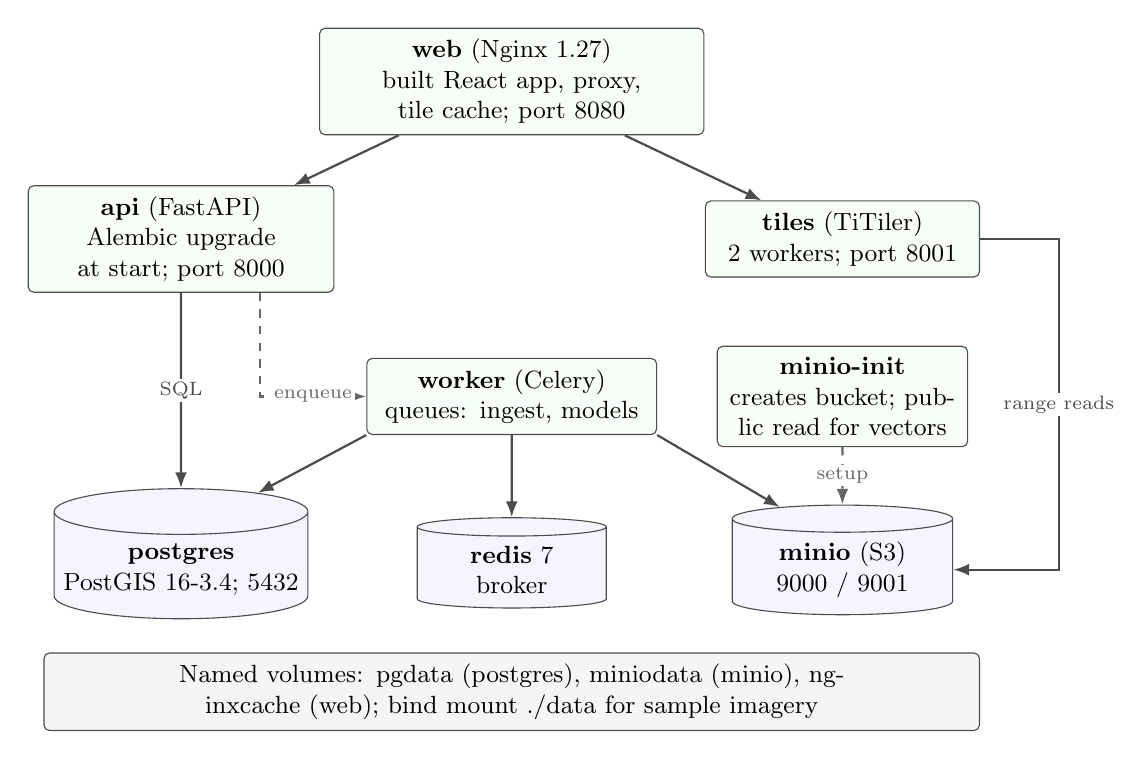
\begin{tikzpicture}[every node/.style={font=\scriptsize}]
\node[box, text width=4.6cm] (web) at (0,0) {\textbf{web} (Nginx 1.27)\\built React app, proxy, tile cache; port 8080};
\node[box, text width=3.6cm] (api) at (-4.2,-2.0) {\textbf{api} (FastAPI)\\Alembic upgrade at start; port 8000};
\node[box, text width=3.2cm] (tiles) at (4.2,-2.0) {\textbf{tiles} (TiTiler)\\2 workers; port 8001};
\node[box, text width=3.4cm] (worker) at (0,-4.0) {\textbf{worker} (Celery)\\queues: ingest, models};
\node[box, text width=2.9cm] (init) at (4.2,-4.0) {\textbf{minio-init}\\creates bucket; public read for vectors};
\node[dbox, minimum width=3.0cm] (pg) at (-4.2,-6.2) {\textbf{postgres}\\PostGIS 16-3.4; 5432};
\node[dbox, minimum width=2.4cm] (redis) at (0,-6.2) {\textbf{redis} 7\\broker};
\node[dbox, minimum width=2.8cm] (minio) at (4.2,-6.2) {\textbf{minio} (S3)\\9000 / 9001};
\node[box, text width=11.6cm, fill=gray!8] (vol) at (0,-7.75) {Named volumes: pgdata (postgres), miniodata (minio), nginxcache (web); bind mount ./data for sample imagery};
\draw[arr] (web) -- (api); \draw[arr] (web) -- (tiles);
\draw[arr] (api) -- node[lbl]{SQL} (pg);
\draw[darr] (api.south) ++(1.0,0) |- node[lbl,pos=0.75]{enqueue} (worker.west);
\draw[arr] (worker) -- (redis);
\draw[arr] (worker.south west) -- (pg.north east);
\draw[arr] (worker.south east) -- (minio.north west);
\draw[arr] (tiles.east) -- ++(1.0,0) |- node[lbl,pos=0.25]{range reads} (minio.east);
\draw[darr] (init) -- node[lbl]{setup} (minio);
\end{tikzpicture}
\caption{Deployment view of the Docker Compose stack}
\label{fig:deploy}
\end{figure}

\begin{figure}[htbp]
\centering
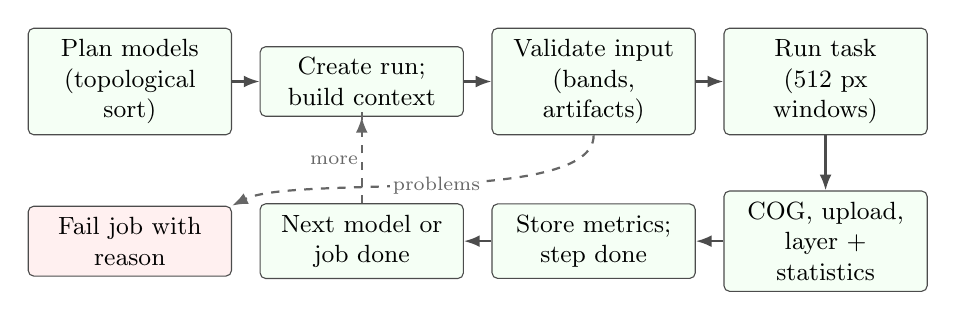
\begin{tikzpicture}[node distance=0.35cm, every node/.style={font=\scriptsize}]
\node[box, text width=2.3cm] (p1) {Plan models\\(topological sort)};
\node[box, text width=2.3cm, right=of p1] (p2) {Create run;\\build context};
\node[box, text width=2.3cm, right=of p2] (p3) {Validate input\\(bands, artifacts)};
\node[box, text width=2.3cm, right=of p3] (p4) {Run task\\(512 px windows)};
\node[box, text width=2.3cm, below=0.7cm of p4] (p5) {COG, upload,\\layer + statistics};
\node[box, text width=2.3cm, left=of p5] (p6) {Store metrics;\\step done};
\node[box, text width=2.3cm, left=of p6] (p7) {Next model or\\job done};
\node[box, text width=2.3cm, left=of p7, fill=red!6] (p8) {Fail job with\\reason};
\draw[arr] (p1)--(p2); \draw[arr] (p2)--(p3); \draw[arr] (p3)--(p4); \draw[arr] (p4)--(p5);
\draw[arr] (p5)--(p6); \draw[arr] (p6)--(p7);
\draw[darr] (p3.south) .. controls +(0,-0.9) and +(0.8,0.4) .. node[lbl,pos=0.5]{problems} (p8.north east);
\draw[darr] (p7.north) -- node[lbl,left]{more} (p7.north |- p2.south) -- (p2.south);
\end{tikzpicture}
\caption{Activity of a model run inside the worker}
\label{fig:activity}
\end{figure}

\begin{figure}[htbp]
\centering
\fbox{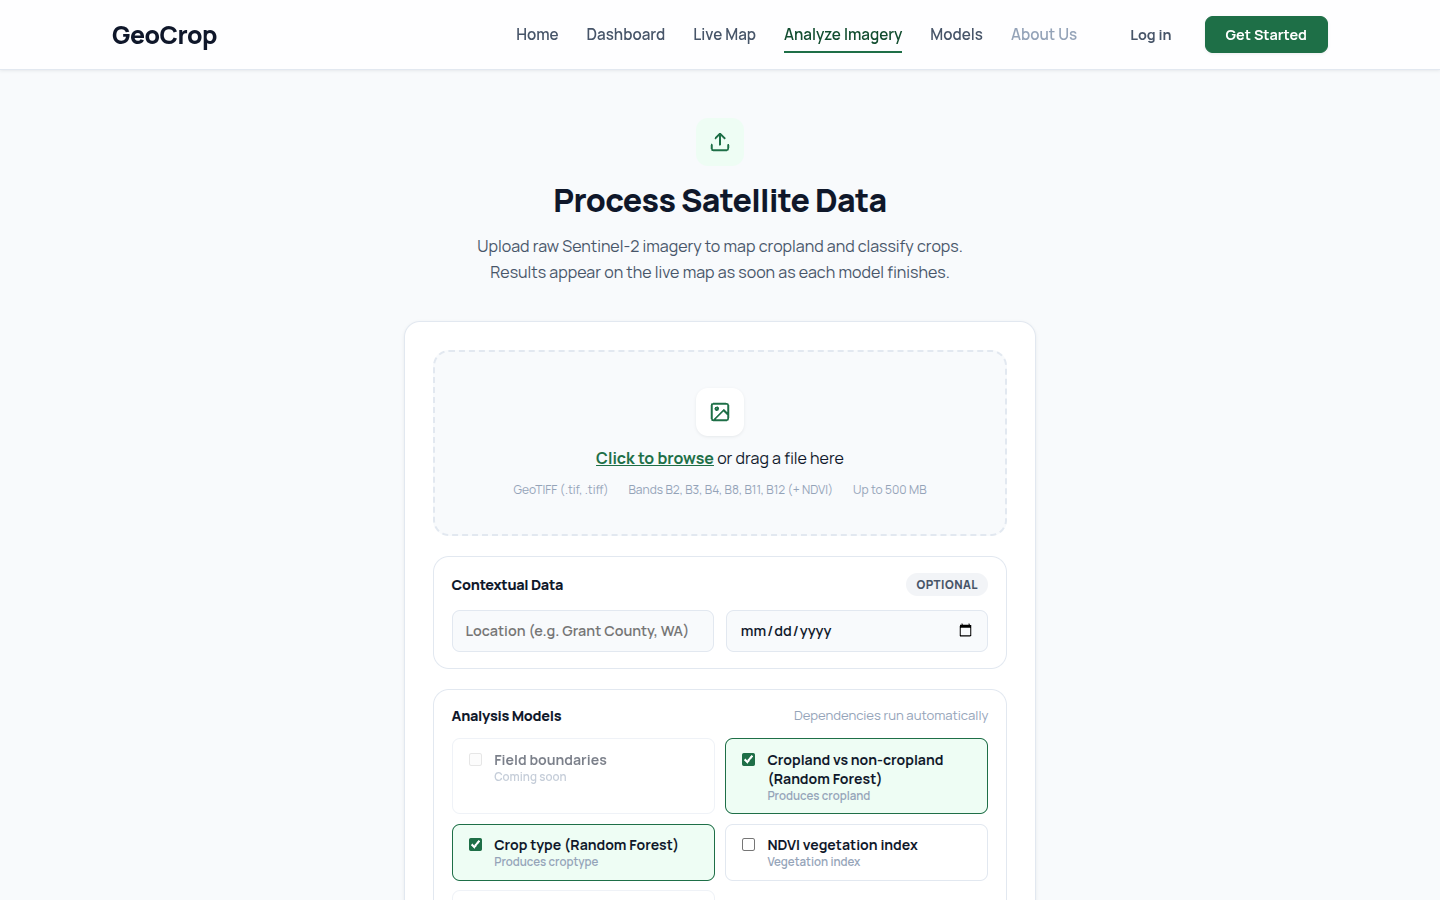
\includegraphics[width=0.88\textwidth]{figures/shot_analyze.png}}
\caption{Analyze Imagery: drag-and-drop upload, contextual data and model selection}
\label{fig:shot-analyze}
\end{figure}

\begin{figure}[htbp]
\centering
\fbox{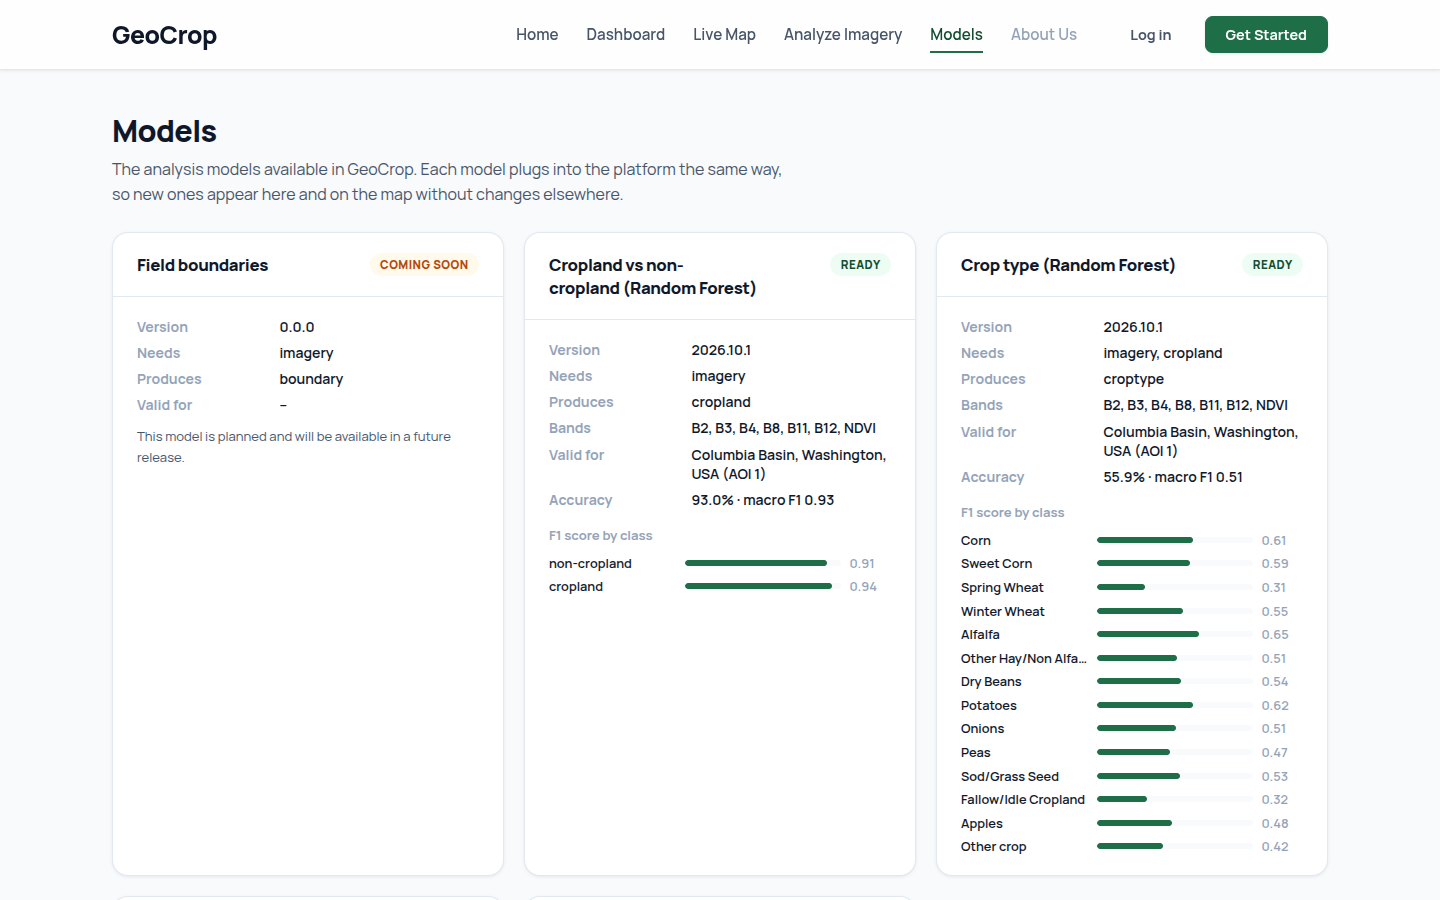
\includegraphics[width=0.88\textwidth]{figures/shot_models.png}}
\caption{Models page: registered models, status, accuracy and F1 per class}
\label{fig:shot-models}
\end{figure}

% ================================================================== F
\chapter{Meeting and Progress Evidence}\label{app:meetings}
\begin{table}[htbp]
\centering\small
\caption{Progress evidence from dated project artefacts}
\label{tab:progressevidence}
\begin{tabularx}{\textwidth}{L{2.4cm} Y L{4.2cm}}
\toprule
\textbf{Date (2026)} & \textbf{Progress} & \textbf{Artefact}\\
\midrule
1--8 Sep & Proposal-stage prototype implemented & Prototype repository commits\\
7--8 Sep & Proposal written & Proposal document and \LaTeX{} source\\
11 Sep & Proposal defence & Proposal slides (F26-155-GeoCrop)\\
14 Sep & Defence result: Approved with Minor Modifications; panel comments P1--P7 & FYP Committee e-mail\\
Sep--Oct & Crop-type experiments, runs 1--3 & Research notebooks\\
14 Oct & Crop-type results and paper comparison & Results report (prepared by Saneed Ullah)\\
14 Oct & Platform architecture implemented and verified & Platform repository commits; benchmark\\
15 Oct & Workflow resource measurement (P4) & Measurement script; Table~\ref{tab:resources}\\
15 Oct & Mid-report & This document\\
\bottomrule
\end{tabularx}
\end{table}

\begin{table}[htbp]
\centering\small
\caption{Supervisor meeting record (to be completed and signed by the team)}
\label{tab:meetings}
\begin{tabularx}{\textwidth}{L{2.0cm} L{3.0cm} Y L{2.6cm}}
\toprule
\textbf{Date} & \textbf{Attendees} & \textbf{Discussion and decisions} & \textbf{Supervisor signature}\\
\midrule
 & & & \\[0.8cm]
 & & & \\[0.8cm]
 & & & \\[0.8cm]
\bottomrule
\end{tabularx}
\end{table}

Open questions prepared for the supervisors: (1) whether LightGBM with neighbourhood inputs and a
3$\times$3 vote is accepted as GeoCrop's crop-type model; (2) whether the final comparison with the
papers should use the CDL confidence filter, reported next to the all-pixel score; (3) whether
field-level classification with field boundaries or the cross-area test should come first.


\cleardoublepage
\phantomsection
\addcontentsline{toc}{chapter}{Bibliography}
\begin{thebibliography}{99}

\bibitem{lin2022}
L.~Lin, L.~Di, C.~Zhang, L.~Guo, Y.~Di, H.~Li, and A.~Yang, ``Validation and refinement of cropland
data layer using a spatial-temporal decision tree algorithm,'' \textit{Scientific Data}, vol.~9,
art.~63, 2022. doi: \href{https://doi.org/10.1038/s41597-022-01169-w}{10.1038/s41597-022-01169-w}.

\bibitem{hao2020}
P.~Hao, L.~Di, C.~Zhang, and L.~Guo, ``Transfer learning for crop classification with Cropland Data
Layer data (CDL) as training samples,'' \textit{Science of the Total Environment}, vol.~733,
art.~138869, 2020. doi: \href{https://doi.org/10.1016/j.scitotenv.2020.138869}{10.1016/j.scitotenv.2020.138869}.

\bibitem{tran2022}
K.~H.~Tran, H.~K.~Zhang, J.~T.~McMaine, X.~Zhang, and D.~Luo, ``10~m crop type mapping using
Sentinel-2 reflectance and 30~m cropland data layer product,'' \textit{International Journal of
Applied Earth Observation and Geoinformation}, vol.~107, art.~102692, 2022.
doi: \href{https://doi.org/10.1016/j.jag.2022.102692}{10.1016/j.jag.2022.102692}.

\bibitem{wang2020}
S.~Wang, S.~Di~Tommaso, J.~M.~Deines, and D.~B.~Lobell, ``Mapping twenty years of corn and soybean
across the US Midwest using the Landsat archive,'' \textit{Scientific Data}, vol.~7, art.~307, 2020.
doi: \href{https://doi.org/10.1038/s41597-020-00646-4}{10.1038/s41597-020-00646-4}.

\bibitem{khan2023}
H.~R.~Khan, Z.~Gillani, M.~H.~Jamal, A.~Athar, M.~T.~Chaudhry, H.~Chao, Y.~He, and M.~Chen, ``Early
identification of crop type for smallholder farming systems using deep learning on time-series
Sentinel-2 imagery,'' \textit{Sensors}, vol.~23, no.~4, art.~1779, 2023.
doi: \href{https://doi.org/10.3390/s23041779}{10.3390/s23041779}.

\bibitem{latif2023}
R.~M.~A.~Latif, J.~He, and M.~Umer, ``Mapping cropland extent in Pakistan using machine learning
algorithms on Google Earth Engine cloud computing framework,'' \textit{ISPRS International Journal of
Geo-Information}, vol.~12, no.~2, art.~81, 2023.
doi: \href{https://doi.org/10.3390/ijgi12020081}{10.3390/ijgi12020081}.

\bibitem{muqaddas2024}
S.~Muqaddas, W.~S.~Qureshi, H.~Jabbar, A.~Munir, and A.~Haider, ``A comprehensive deep learning
approach for harvest ready sugarcane pixel classification in Punjab, Pakistan using Sentinel-2
multispectral imagery,'' \textit{Remote Sensing Applications: Society and Environment}, vol.~35,
art.~101225, 2024. doi: \href{https://doi.org/10.1016/j.rsase.2024.101225}{10.1016/j.rsase.2024.101225}.

\bibitem{edri2026}
A.~Edri, Y.~Edan, L.~Fine, O.~Rozenstein, and T.~Paz-Kagan, ``Scalable field boundary refinement from
satellite time series using deep learning,'' \textit{Precision Agriculture}, vol.~27, art.~111, 2026.
doi: \href{https://doi.org/10.1007/s11119-026-10413-x}{10.1007/s11119-026-10413-x}.

\bibitem{desloires2023}
J.~Desloires, D.~Ienco, and A.~Botrel, ``Out-of-year corn yield prediction at field-scale using
Sentinel-2 satellite imagery and machine learning methods,'' \textit{Computers and Electronics in
Agriculture}, vol.~209, art.~107807, 2023.
doi: \href{https://doi.org/10.1016/j.compag.2023.107807}{10.1016/j.compag.2023.107807}.

\bibitem{xiao2024}
G.~Xiao, X.~Zhang, Q.~Niu, X.~Li, X.~Li, L.~Zhong, and J.~Huang, ``Winter wheat yield estimation at the
field scale using Sentinel-2 data and deep learning,'' \textit{Computers and Electronics in
Agriculture}, vol.~216, art.~108555, 2024.
doi: \href{https://doi.org/10.1016/j.compag.2023.108555}{10.1016/j.compag.2023.108555}.

\bibitem{you2017}
J.~You, X.~Li, M.~Low, D.~B.~Lobell, and S.~Ermon, ``Deep Gaussian process for crop yield prediction
based on remote sensing data,'' in \textit{Proc.\ AAAI Conference on Artificial Intelligence}, 2017,
pp.~4559--4565. doi: \href{https://doi.org/10.1609/aaai.v31i1.11172}{10.1609/aaai.v31i1.11172}.

\bibitem{zhang2025}
H.~K.~Zhang, Y.~Shen, X.~Zhang, J.~Li, Z.~Yang, Y.~Xu, C.~Zhang, L.~Di, and D.~P.~Roy, ``Robust and
timely within-season conterminous United States crop type mapping using Landsat Sentinel-2 time
series and the transformer architecture,'' \textit{Remote Sensing of Environment}, vol.~329,
art.~114950, 2025. doi: \href{https://doi.org/10.1016/j.rse.2025.114950}{10.1016/j.rse.2025.114950}.

\bibitem{li2024}
H.~Li, L.~Di, C.~Zhang, L.~Lin, L.~Guo, E.~G.~Yu, and Z.~Yang, ``Automated in-season crop-type data
layer mapping without ground truth for the conterminous United States based on multisource satellite
imagery,'' \textit{IEEE Transactions on Geoscience and Remote Sensing}, vol.~62, art.~4403214, 2024.
doi: \href{https://doi.org/10.1109/TGRS.2024.3361895}{10.1109/TGRS.2024.3361895}.

\bibitem{szwarcman2024}
D.~Szwarcman \textit{et al.}, ``Prithvi-EO-2.0: A versatile multi-temporal foundation model for Earth
observation applications,'' arXiv:2412.02732, 2024.

\bibitem{garnot2020}
V.~Sainte~Fare~Garnot, L.~Landrieu, S.~Giordano, and N.~Chehata, ``Satellite image time series
classification with pixel-set encoders and temporal self-attention,'' in \textit{Proc.\ IEEE/CVF
Conference on Computer Vision and Pattern Recognition (CVPR)}, 2020. arXiv:1911.07757.

\bibitem{tseng2023}
G.~Tseng, R.~Cartuyvels, I.~Zvonkov, M.~Purohit, D.~Rolnick, and H.~Kerner, ``Lightweight, pre-trained
transformers for remote sensing timeseries,'' arXiv:2304.14065, 2023.

\bibitem{russwurm2020}
M.~Ru{\ss}wurm, C.~Pelletier, M.~Z{\"o}llner, S.~Lef{\`e}vre, and M.~K{\"o}rner, ``BreizhCrops: A time
series dataset for crop type mapping,'' \textit{ISPRS Archives}, vol.~XLIII-B2-2020, pp.~1545--1551,
2020. doi: \href{https://doi.org/10.5194/isprs-archives-XLIII-B2-2020-1545-2020}{10.5194/isprs-archives-XLIII-B2-2020-1545-2020}.

\bibitem{pelletier2019}
C.~Pelletier, G.~I.~Webb, and F.~Petitjean, ``Temporal convolutional neural network for the
classification of satellite image time series,'' \textit{Remote Sensing}, vol.~11, no.~5, art.~523,
2019. doi: \href{https://doi.org/10.3390/rs11050523}{10.3390/rs11050523}.

\bibitem{ke2017}
G.~Ke, Q.~Meng, T.~Finley, T.~Wang, W.~Chen, W.~Ma, Q.~Ye, and T.-Y.~Liu, ``LightGBM: A highly
efficient gradient boosting decision tree,'' in \textit{Advances in Neural Information Processing
Systems}, vol.~30, 2017.

\bibitem{zhang2019}
C.~Zhang, L.~Di, L.~Lin, and L.~Guo, ``Machine-learned prediction of annual crop planting in the U.S.
Corn Belt based on historical crop planting maps,'' \textit{Computers and Electronics in
Agriculture}, vol.~166, art.~104989, 2019.
doi: \href{https://doi.org/10.1016/j.compag.2019.104989}{10.1016/j.compag.2019.104989}.

\bibitem{cog}
Cloud Optimized GeoTIFF, ``COG specification and documentation,'' 2026. [Online]. Available:
\url{https://cogeo.org}.

\bibitem{titiler}
Development Seed, ``TiTiler: a modern dynamic tile server built on FastAPI and Rasterio/GDAL,''
2026. [Online]. Available: \url{https://developmentseed.org/titiler/}.

\bibitem{pmtiles}
Protomaps, ``PMTiles: a single-file archive format for tiled data,'' 2026. [Online]. Available:
\url{https://docs.protomaps.com/pmtiles/}.

\bibitem{maplibre}
MapLibre, ``MapLibre GL JS documentation,'' 2026. [Online]. Available: \url{https://maplibre.org}.

\bibitem{postgis}
PostGIS Project, ``PostGIS: spatial and geographic objects for PostgreSQL,'' 2026. [Online].
Available: \url{https://postgis.net}.

\bibitem{sentinel2}
European Space Agency, ``Sentinel-2 mission overview,'' 2026. [Online]. Available:
\url{https://sentiwiki.copernicus.eu/web/s2-mission}.

\bibitem{cdlsite}
USDA National Agricultural Statistics Service, ``Cropland Data Layer,'' 2026. [Online]. Available:
\url{https://www.nass.usda.gov/Research_and_Science/Cropland/SARS1a.php}.

\bibitem{seoulaccord2026}
Seoul Accord, ``Section D -- Graduate attributes: D.4 Common range and contextual definitions,''
2026. [Online]. Available: \url{https://www.seoulaccord.org/document.php?id=79}.

\bibitem{onesoil2026}
OneSoil, ``OneSoil platform: field monitoring, productivity analysis and precision agriculture,''
2026. [Online]. Available: \url{https://onesoil.ai/en/platform}.

\end{thebibliography}


\end{document}
